% **************************************************************************************************************
% A Classic Thesis Style
% An Homage to The Elements of Typographic Style
%
% Copyright (C) 2010 Andr� Miede http://www.miede.de
%
% If you like the style then I would appreciate a postcard. My address 
% can be found in the file ClassicThesis.pdf. A collection of the 
% postcards I received so far is available online at 
% http://postcards.miede.de
%
% License:
% This program is free software; you can redistribute it and/or modify
% it under the terms of the GNU General Public License as published by
% the Free Software Foundation; either version 2 of the License, or
% (at your option) any later version.
%
% This program is distributed in the hope that it will be useful,
% but WITHOUT ANY WARRANTY; without even the implied warranty of
% MERCHANTABILITY or FITNESS FOR A PARTICULAR PURPOSE.  See the
% GNU General Public License for more details.
%
% You should have received a copy of the GNU General Public License
% along with this program; see the file COPYING.  If not, write to
% the Free Software Foundation, Inc., 59 Temple Place - Suite 330,
% Boston, MA 02111-1307, USA.
%
% **************************************************************************************************************
% Note:
%    * You must not use "u etc. in strings/commands that will be spaced out (use \"u or real umlauts instead)
%    * New enumeration (small caps): \begin{aenumerate} \end{aenumerate}
%    * For margin notes: \graffito{}
%    * Do not use bold fonts in this style, it is designed around them
%    * Use tables as in the examples
%    * See classicthesis-ldpkg.sty for useful commands
% **************************************************************************************************************
% To Do:
%    * [high] Check this out: http://www.golatex.de/koma-script-warnung-in-verbindung-mit-listings-package-t2058.html
%    * [medium] mathbb in section-titles/chapter-titles => disappears somehow in headlines!!!
%    * [low] Calculate text block size for Libertine font
%    * [low] Think about processing a4paper, a5paper, 10pt, 11pt, 12pt etc. options for typearea layout
%            (store values in internal variables and handle by \AtEndOfPackage{\areaset...})
% **************************************************************************************************************
\documentclass[ twoside,openright,titlepage,fleqn,numbers=noenddot,headinclude,%1headlines,footinclude
                11pt,letterpaper,BCOR5mm,cleardoublepage=empty,abstractoff % <--- obsolete, remove (todo)
                ]{scrreprt}
% ********************************************************************
% Development Stuff
% ********************************************************************
\listfiles
%\usepackage[l2tabu, orthodox, abort]{nag}
%\usepackage[warning, all]{onlyamsmath}
% ********************************************************************
% Re-usable information
% ********************************************************************
\newcommand{\myTitle}{A Substrate for Accountable Layered Systems\xspace}
\newcommand{\myDegree}{Ph.D. in the Media Arts and Sciences\xspace}
\newcommand{\myName}{Bo Morgan\xspace}
\newcommand{\myProf}{Marvin Minsky\xspace}
\newcommand{\myOtherProf}{Gerald Sussman\xspace}
\newcommand{\mySupervisor}{Joseph Paradiso\xspace}
\newcommand{\myFaculty}{Put data here\xspace}
\newcommand{\myDepartment}{Media Lab\xspace}
\newcommand{\myUni}{\protect{Massachusetts Institute of Technology}\xspace}
\newcommand{\myLocation}{Cambridge\xspace}
\newcommand{\myTime}{May 2012\xspace}
\newcommand{\myVersion}{Version 0.1\xspace}
%*******************************************************
% Packages with options that might require adjustments
%*******************************************************
\usepackage[latin1]{inputenc}
\usepackage[ngerman,american]{babel}
\usepackage{natbib}
%\usepackage[square,numbers]{natbib}
\usepackage[fleqn]{amsmath} % math environments and more by the AMS

%*******************************************************
\usepackage{classicthesis-ldpkg} % [backref]
%*******************************************************
% Options for classicthesis.sty:
% tocaligned eulerchapternumbers drafting linedheaders listsseparated 
% subfig nochapters beramono eulermath parts minionpro pdfspacing 
% listings dottedtoc minionprospacing manychapters
\usepackage[eulerchapternumbers,drafting,listings,listsseparated,%pdfspacing,%listings,
            subfig,beramono,eulermath,parts,manychapters]{classicthesis}

%*******************************************************
% Some font experiments
%*******************************************************
%\usepackage[osf]{libertine}
%\usepackage{hfoldsty}
%\usepackage[light,condensed,math]{iwona}
%\renewcommand{\sfdefault}{iwona}
%\usepackage{lmodern} % <-- no osf support :-(
%\usepackage[urw-garamond]{mathdesign} <-- no osf support :-(

%*******************************************************
% Fine-tuning for the text area
%*******************************************************
%\linespread{1.05} % a bit more for Palatino
%\areaset[5mm]{312pt}{761pt} % 686 (factor 2.2) + 33 head + 42 head \the\footskip
%\setlength{\marginparwidth}{7em}%
%\setlength{\marginparsep}{2em}%

%*******************************************************
% hack to use citations in float environments 
% will be fixed with caption package version 3.2
%*******************************************************
\usepackage{makerobust} 
\makeatletter 
%\MakeRobustCommand\caption@xref 
\makeatother 


% BEGIN FIBR EXPRESSION CODE
\usepackage{amsthm}
\newtheorem{expression}{Expression}[section]



% END FIBR EXPRESSION CODE



% BEGIN DRAFT WATERMARK CODE
%
% This code is from
% http://filoxus.blogspot.com/2008_01_01_archive.html
%
% Thanks to the ``Daily rant: A random blog about everything, mostly
% programming''

\usepackage{graphicx}
\usepackage{type1cm}
\usepackage{eso-pic}
\usepackage{color}

\makeatletter
\AddToShipoutPicture{
  \setlength{\@tempdimb}{.5\paperwidth}
  \setlength{\@tempdimc}{.5\paperheight}
  \setlength{\unitlength}{1pt}
  \put(\strip@pt\@tempdimb,\strip@pt\@tempdimc){
%    \makebox(0,0){
%      \rotatebox{45}{
%        \makebox(-72,0){
%          \vspace{3cm}\textcolor[gray]{0.875}{{\fontsize{3cm}{3cm}\selectfont{UNOFFICIAL}}}
%        }
%      }
%    }
%    \makebox(0,0){
%      \rotatebox{45}{
%        \makebox(-72,0){
%          \vspace{-6cm}\textcolor[gray]{0.875}{{\fontsize{6cm}{6cm}\selectfont{DRAFT}}}
%        }
%      }
%    }
    \makebox(0,0){
      \rotatebox{45}{
        \vspace{-6cm}\textcolor[gray]{0.9375}{{\fontsize{6cm}{6cm}\selectfont{DRAFT}}}
      }
    }
  }
}
\makeatother

% END DRAFT WATERMARK CODE


%*******************************************************            
%\usepackage[section,below]{placeins} <--- not everybody wants this
%\usepackage[all]{hypcap} <--- does not work with MiKTeX 2.6
% ********************************************************************
% Language/strings for backrefs (change here, thanks, Lorenzo)
%*******************************************************
%\renewcommand{\backrefnotcitedstring}{\relax}%(Not cited.)
%\renewcommand{\backrefcitedsinglestring}[1]{(Citato a pagina~#1.)}
%\renewcommand{\backrefcitedmultistring}[1]{(Citato alle pagine~#1.)}
%\renewcommand{\backreftwosep}{ e~}
%\renewcommand{\backreflastsep}{ e~}
% ********************************************************************
% Setup and Finetuning
%*******************************************************
\newlength{\abcd} % for ab..z string length calculation
\newcommand{\myfloatalign}{\centering} % how all the floats will be aligned
\setlength{\extrarowheight}{3pt} % increase table row height
% ********************************************************************
% Captions look and feel
%*******************************************************
\captionsetup{format=hang,font=small}
% ********************************************************************
% Listings setup
% ********************************************************************
%\lstset{emph={trueIndex,root},emphstyle=\color{BlueViolet}}%\underbar} % for special keywords
% ********************************************************************
\lstset{language=[LaTeX]Tex,%C++,
    keywordstyle=\color{RoyalBlue},%\bfseries,
    basicstyle=\small\ttfamily,
    %identifierstyle=\color{NavyBlue},
    commentstyle=\color{Green}\ttfamily,
    stringstyle=\rmfamily,
    numbers=none,%left,%
    numberstyle=\scriptsize,%\tiny
    stepnumber=5,
    numbersep=8pt,
    showstringspaces=false,
    breaklines=true,
    frameround=ftff,
    frame=single,
    belowcaptionskip=.75\baselineskip,
    %numberbychapter=false
    %frame=L
}

% ********************************************************************
% Where to look for graphics
%*******************************************************
%\graphicspath{{gfx/}{misc/}} % considered harmful according to l2tabu
% ********************************************************************
% Hyperreferences
%*******************************************************
\hypersetup{%
    colorlinks=true, linktocpage=true, pdfstartpage=3, pdfstartview=FitV,%
    % uncomment the following line if you want to have black links (e.g., for printing)
    %colorlinks=false, linktocpage=false, pdfborder={0 0 0}, pdfstartpage=3, pdfstartview=FitV,% 
    breaklinks=true, pdfpagemode=UseNone, pageanchor=true, pdfpagemode=UseOutlines,%
    plainpages=false, bookmarksnumbered, bookmarksopen=true, bookmarksopenlevel=0,%
    hypertexnames=true, pdfhighlight=/O,%hyperfootnotes=true,%nesting=true,%frenchlinks,%
    urlcolor=webbrown, linkcolor=RoyalBlue, citecolor=webgreen, %pagecolor=RoyalBlue,%
    %urlcolor=Black, linkcolor=Black, citecolor=Black, %pagecolor=Black,%
    pdftitle={\myTitle},%
    pdfauthor={\textcopyright\ \myName, \myUni, \myFaculty},%
    pdfsubject={},%
    pdfkeywords={},%
    pdfcreator={pdfLaTeX},%
    pdfproducer={LaTeX, hyperref, classicthesis, LibreDraw, and GraphViz}%
}








% BEGIN LONG DIVISION DIGIT SPACING
%
\newdimen\digitwidth
\settowidth\digitwidth{0}
\def~{\hspace{\digitwidth}}

\def\longdivisionrule#1#2{%
\noalign{\moveright#1\digitwidth%
\vbox{\hrule width#2\digitwidth}}}

%101\,\begin{tabular}[b]{@{}r@{}}
%10010 \\ \hline
%\big)\begin{tabular}[t]{@{}l@{}}
%1011110 \\
%101 \\ \longdivisionrule{0}{7}
%~~~111 \\
%~~~101 \\ \longdivisionrule{3}{4}
%~~~~100
%\end{tabular}
%\end{tabular}
%
% END LONG DIVISION DIGIT SPACING


% BEGIN EQUATION SECTION NUMBERING
%
%\numberwithin{equation}{section}
%
% END EQUATION SECTION NUMBERING








%********************************************************************
% Hyphenation
%*******************************************************
%\hyphenation{put special hyphenation here}
% ********************************************************************
% GO!GO!GO! MOVE IT!
%*******************************************************
\begin{document}
\frenchspacing
\raggedbottom
\selectlanguage{american} % american ngerman
%\renewcommand*{\bibname}{new name}
%\setbibpreamble{}
\pagenumbering{roman}
\pagestyle{plain}
%********************************************************************
% Frontmatter
%*******************************************************
%*******************************************************
% Little Dirty Titlepage
%*******************************************************
\thispagestyle{empty}
%\pdfbookmark[1]{Titel}{title}
%*******************************************************
\begin{center}
    \spacedlowsmallcaps{\myName} \\ \medskip                        

    \begingroup
        \color{Maroon}\spacedallcaps{\myTitle}
    \endgroup
\end{center}        

\makebox[7in]{
  {\flushright{Advisor\hspace{0.5cm}          \makebox[3in]{\hrulefill}}}
  
  {\flushright{Committee Member\hspace{0.5cm} \makebox[3in]{\hrulefill}}}
}

%*******************************************************
% Titlepage
%*******************************************************
\begin{titlepage}
	% if you want the titlepage to be centered, uncomment and fine-tune the line below (KOMA classes environment)
	\begin{addmargin}[-1cm]{-3cm}
    \begin{center}
        \large  

        \hfill

        \vfill

        \begingroup
            \color{Maroon}\spacedallcaps{\myTitle} \\ \bigskip
        \endgroup

        \spacedlowsmallcaps{\myName}

        \vfill

        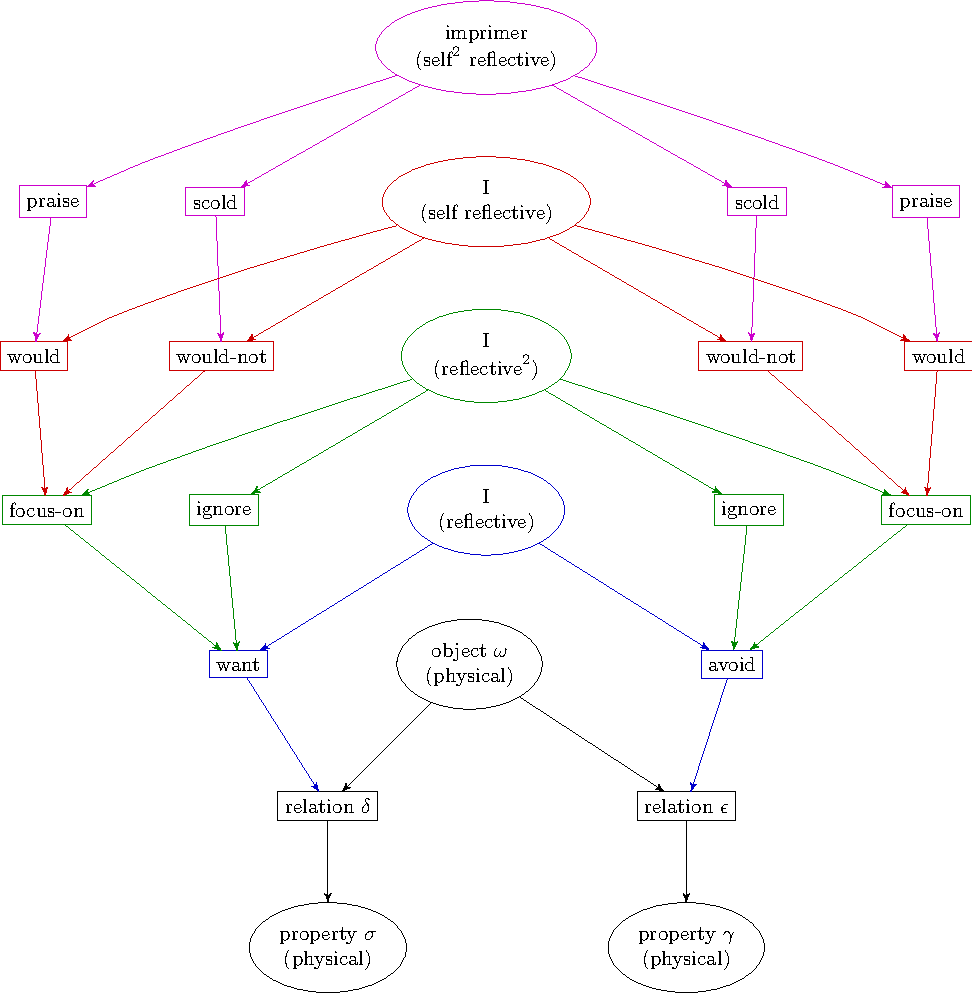
\includegraphics[width=4cm]{gfx/model-6} \\ \medskip

        \myDegree \\ \medskip   
        %\myDepartment \\                            
        %\myFaculty \\
        %\myUni \\ \bigskip

        \myTime

        \vfill                      

    \end{center}  
  \end{addmargin}       
\end{titlepage}   

\thispagestyle{empty}

\hfill

\vfill

\noindent\myName: \textit{\myTitle,} \myDegree, \textcopyright\ \myTime

%\bigskip
%
%\noindent\spacedlowsmallcaps{Supervisors}: \\
%\myProf \\
%\myOtherProf \\ 
%\mySupervisor
%
%\medskip
%
%\noindent\spacedlowsmallcaps{Location}: \\
%\myLocation
%
%\medskip
%
%\noindent\spacedlowsmallcaps{Time Frame}: \\
%\myTime

\cleardoublepage%*******************************************************
% Dedication
%*******************************************************
\thispagestyle{empty}
%\phantomsection 
\refstepcounter{dummy}
\pdfbookmark[1]{Dedication}{Dedication}

\vspace*{3cm}

%\begin{center}
%``If wishes were horses, beggars would ride.''  Since they are not, \\ \medskip
%since really to satisfy an impulse or interest means to work it out, \\ \medskip
%and working it out involves running up against obstacles, \\ \medskip
%becoming acquainted with materials, exercising ingenuity, \\ \medskip
%patience, persistence, alertness, it of necessity involves \\ \medskip
%discipline---ordering of power and supplies knowledge. \\ \medskip
%    --- \defcitealias{dewey:1907}{John Dewey}\citetalias{dewey:1907}
%\end{center}
%
%\medskip

%
%Though there be no such thing as Chance in the world; \\
%our ignorance of the real cause of any event \\
%has the same influence on the understanding, \\
%and begets a like species of belief or opinion.} \\ \medskip
%    --- \defcitealias{hume:1902}{David Hume}\citetalias{hume:1902}
%
%
%

\begin{center}
Though there be no such thing as Chance in the world; \\
our ignorance of the real cause of any event \\
has the same influence on the understanding, \\
and begets a like species of belief or opinion. \\ \medskip
    --- \defcitealias{hume:1902}{David Hume}\citetalias{hume:1902}
\end{center}

\medskip

\begin{center}
    Dedicated to the loving memory of Pushpinder Singh. \\ \smallskip
    1972\,--\,2006
\end{center}

\cleardoublepage%*******************************************************
% Abstract
%*******************************************************
%\renewcommand{\abstractname}{Abstract}
\pdfbookmark[1]{Abstract}{Abstract}
\begingroup
\let\clearpage\relax
\let\cleardoublepage\relax
\let\cleardoublepage\relax

\chapter*{Abstract}

There have been two directions of research with the goal of building a
machine that explains intelligent human behavior.  The first approach
is to build a baby-machine that learns from scratch to accomplish
goals through interactions with its environment.  The second approach
is to give the machine an abundance of knowledge that represents
correct behavior.

Each of these solutions has benefits and drawbacks.  The baby-machine
approach is good for dealing with novel problems, but these problems
are necessarily simple because complex problems require a lot of
background knowledge.  The data abundance approach deals well with
complicated problems requiring a lot of background knowledge, but
fails to adapt to changing environments, for which the algorithm has
not already been trained.

We are working on an algorithm that benefits from both of these
approaches by learning from cultural language knowledge, while
reflectively monitoring and recognizing the failures of this knowledge
when it is used in a goal-oriented domain.

Toward this end we have developed a reflective programming language
allowing us the ability to monitor the execution and interactions
between large numbers of complicated lisp-like processes.  Further, we
have developed a cognitive architecture within our language that
provides structures for layering reflective processes, resulting in a
hierarchy of control algorithms that respond to failures in the layers
below.

Finally, we present an example of our cognitive architecture learning
in the context of a social commonsense reasoning domain with parents
that teach children as they attempt to accomplish cooking tasks in a
kitchen.

\endgroup

\vfill

\cleardoublepage%*******************************************************
% Publications
%*******************************************************
\pdfbookmark[1]{Publications}{publications}
\chapter*{Publications}
Some ideas and figures have appeared previously in the following publications:

\bigskip

\noindent Smith, D. and Morgan, B.; "IsisWorld: An open source
 commonsense simulator for AI researchers"; AAAI 2010 Workshop on
 Metacognition; 2010 April

\vspace{5mm}

\noindent Morgan, B.; ``Moral Compass: Commonsense Social Reasoning
 Cognitive Architecture''; http://em-two.net/about; Commonsense Tech
 Note; MIT Media Lab; 2011 January

\vspace{5mm}

\noindent Morgan, B.; ``A Computational Theory of the Communication of
 Problem Solving Knowledge between Parents and Children''; PhD
 Proposal; MIT Media Lab 2010 January

\vspace{5mm}

\noindent Morgan, B.; ``Funk2: A Distributed Processing Language for 
 Reflective Tracing of a Large Critic-Selector Cognitive
 Architecture''; Proceedings of the Metacognition Workshop at the
 Third IEEE International Conference on Self-Adaptive and
 Self-Organizing Systems; San Francisco, California, USA; 2009
 September

\vspace{5mm}

\noindent Morgan, B.; ``Funk2: A Frame-based Programming Language with
 Causally Reflective Capabilities (draft in progress)''; Technical
 Note; Massachusetts Institute of Technology; 2009 May

\vspace{5mm}

\noindent Morgan, B.; ``Learning Commonsense Human-language Descriptions
 from Temporal and Spatial Sensor-network Data''; Masters Thesis;
 Massachusetts Institute of Technology; 2006 August

\vspace{5mm}

\noindent Morgan, B.; ``Learning perception lattices to compare
 generative explanations of human-language stories''; Published
 Online; Commonsense Tech Note; MIT Media Lab; 2006 July

\vspace{5mm}

\noindent Morgan, B. and Singh, P.; ``Elaborating Sensor Data using
 Temporal and Spatial Commonsense Reasoning''; International Workshop
 on Wearable and Implantable Body Sensor Networks (BSN-2006); 2005
 November

\vspace{5mm}

\noindent Morgan, B.; ``Experts think together to solve hard problems'';
 Published Online; Commonsense Tech Note; MIT Media Lab 2005 August

\vspace{5mm}

\noindent Morgan, B.; ``LifeNet Belief Propagation''; Published Online;
 Commonsense Tech Note; MIT Media Lab; 2004 January

\cleardoublepage%*******************************************************
% Acknowledgments
%*******************************************************
\pdfbookmark[1]{Acknowledgments}{acknowledgments}

%Don't do anything that isn't play. \\ \medskip
%    --- Joseph Campbell



\begin{flushright}{\slshape    
Don't do anything that isn't play.} \\ \medskip
    --- Joseph Campbell
\end{flushright}



\bigskip

\begingroup
\let\clearpage\relax
\let\cleardoublepage\relax
\let\cleardoublepage\relax
\chapter*{Acknowledgments}

I would first like to thank:

\begin{itemize}
\item{Push Singh for being a good friend and advisor.}
\end{itemize}

Next I would like to thank my committee:

\begin{itemize}
\item{Joe Paradiso for unfailing support and faith in my ability to do
  something well.}
\item{Marvin Minsky for consistently and patiently providing an
  inspiringly critical perspective and a wealth of important problems
  to solve.}
\item{Gerry Sussman for loving to program.}
\item{Mike Cox for providing critical direction for navigating the
  space of the contemporary meta-cognitive computational sciences.}
\end{itemize}

I would next like to thank my immediate family:

\begin{itemize}
\item{Greg Morgan and Carolyn Spinner for being supportive parents---willing to help me think about anything at any time.}
\item{Paul Bergman for teaching me how to program.}
\item{Virginia Barasch for painting my finger nails.}
\item{Leaf Morgan for playing Archon with me.}
\end{itemize}

Professors:

\begin{itemize}
\item{Henry Lieberman}
\item{Ed Boyden}
\item{Walter Bender}
\item{Ted Selker}
\end{itemize}

Popes:

\begin{itemize}
\item{Dustin Smith}
\item{Scotty Vercoe}
\item{Dane Scalise}
\end{itemize}

Friends:

\begin{itemize}
\item{Mako Hill}
\item{Barbara Barry}
\end{itemize}

\endgroup


\pagestyle{scrheadings}
\cleardoublepage%*******************************************************
% Table of Contents
%*******************************************************
%\phantomsection
\refstepcounter{dummy}
\pdfbookmark[1]{\contentsname}{tableofcontents}
\setcounter{tocdepth}{2} % <-- 2 includes up to subsections in the ToC
\setcounter{secnumdepth}{3} % <-- 3 numbers up to subsubsections
\manualmark
\markboth{\spacedlowsmallcaps{\contentsname}}{\spacedlowsmallcaps{\contentsname}}
\tableofcontents 
\automark[section]{chapter}
\renewcommand{\chaptermark}[1]{\markboth{\spacedlowsmallcaps{#1}}{\spacedlowsmallcaps{#1}}}
\renewcommand{\sectionmark}[1]{\markright{\thesection\enspace\spacedlowsmallcaps{#1}}}%*******************************************************
% List of Figures and of the Tables
%*******************************************************
\clearpage

\begingroup 
    \let\clearpage\relax
    \let\cleardoublepage\relax
    \let\cleardoublepage\relax
    %*******************************************************
    % List of Figures
    %*******************************************************    
    %\phantomsection 
    \refstepcounter{dummy}
    %\addcontentsline{toc}{chapter}{\listfigurename}
    \pdfbookmark[1]{\listfigurename}{lof}
    \listoffigures

    \vspace*{8ex}

    %*******************************************************
    % List of Tables
    %*******************************************************
    %\phantomsection 
    \refstepcounter{dummy}
    %\addcontentsline{toc}{chapter}{\listtablename}
    \pdfbookmark[1]{\listtablename}{lot}
    \listoftables
        
    \vspace*{8ex}
%   \newpage
    
    %*******************************************************
    % List of Listings
    %*******************************************************      
	  %\phantomsection 
    \refstepcounter{dummy}
    %\addcontentsline{toc}{chapter}{\lstlistlistingname}
    \pdfbookmark[1]{\lstlistlistingname}{lol}
    \lstlistoflistings 

    \vspace*{8ex}
       
    %*******************************************************
    % Acronyms
    %*******************************************************
    %\phantomsection 
    \refstepcounter{dummy}
    \pdfbookmark[1]{Acronyms}{acronyms}
    \markboth{\spacedlowsmallcaps{Acronyms}}{\spacedlowsmallcaps{Acronyms}}
    \chapter*{Acronyms}
    \begin{acronym}[UML]
        \acro{GPS}{General Problem Solver}
    \end{acronym}                     
\endgroup

\cleardoublepage

\cleardoublepage%\manualmark
%\markboth{\spacedlowsmallcaps{Preface}}{\spacedlowsmallcaps{Preface}} % work-around to have small caps also
\refstepcounter{dummy}

%************************************************
\addtocontents{toc}{\protect\vspace{\beforebibskip}} % to have the bib a bit from the rest in the toc
\addcontentsline{toc}{chapter}{\tocEntry{Preface}}
%************************************************

\chapter*{Preface}
\chaptermark{Preface}


%*******************************************************
% Mainmatter
%*******************************************************
\pagenumbering{arabic}
%************************************************
\chapter{Introduction}
\label{chapter:introduction}
%************************************************

An intelligent system thinks about a problem domain, learning the
effects of its actions, constructing and executing plans to accomplish
its goals.  I will refer to these types of thinking about a problem
domain as deliberative thinking.  A reflective intelligence extends
the deliberative intelligence by learning to accomplish goals in its
own deliberative thinking process.  Reflective thinking is sometimes
referred to as ``thinking about thinking'' or ``metacognition.''  A
reflective intelligence can learn to select between different types of
thinking that are appropriate for generating plans toward different
types of goals.  In this thesis, I present the Substrate for
Accountable Layered Systems (SALS), an open-source
\begin{wrapfigure}{r}{6.125cm}
  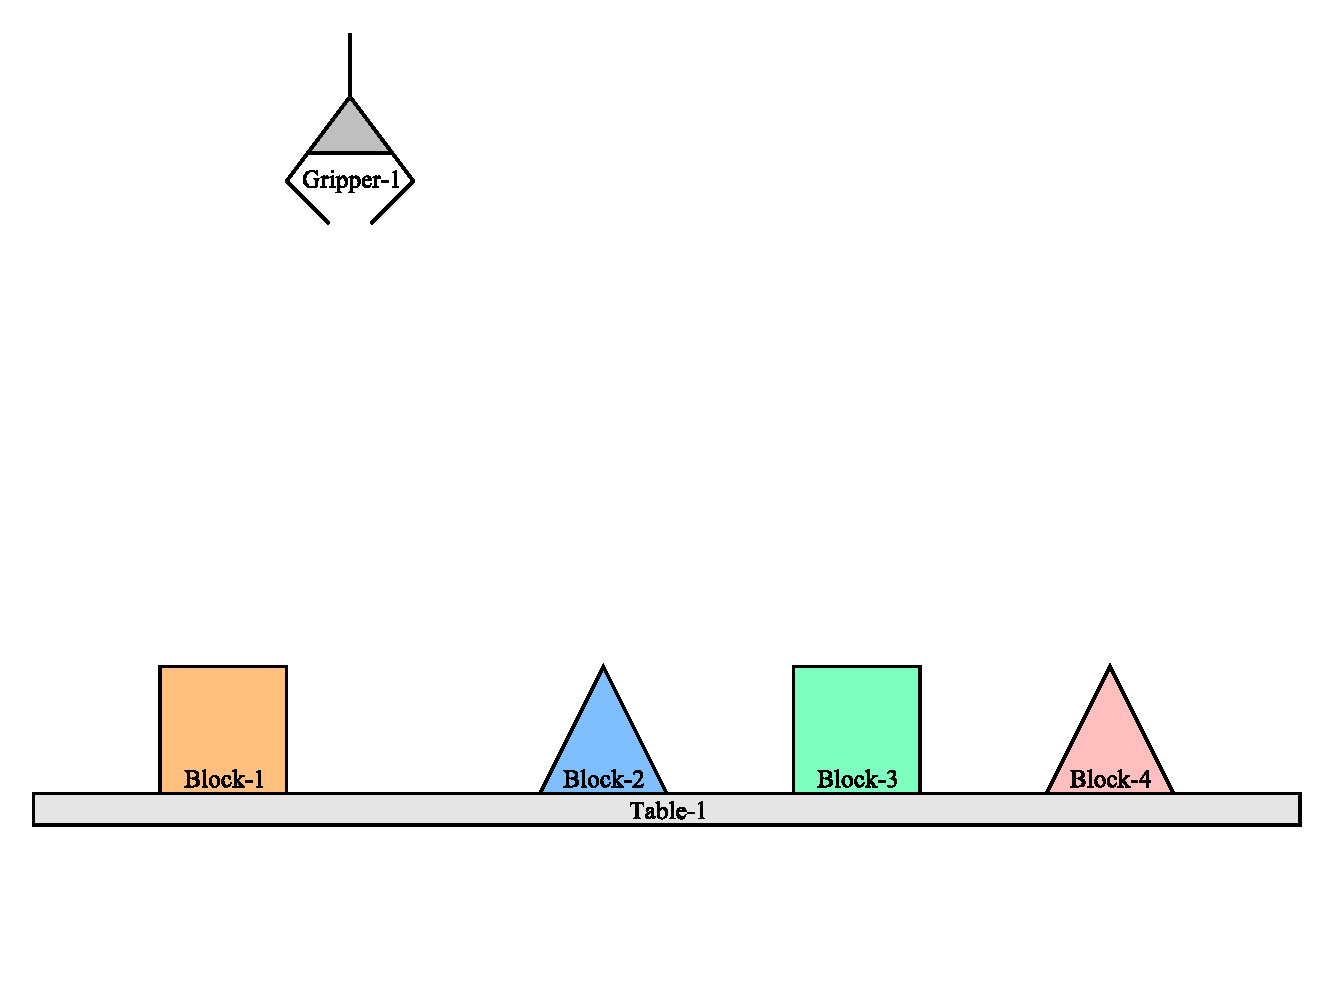
\includegraphics[width=6cm]{gfx/blocks_world_large-01}
  \caption[An example ``Blocks World'' problem domain.]{An example
    ``Blocks World'' problem domain.}
  \label{figure:introduction_example_problem_domain}
\end{wrapfigure}
software platform for the development of experimental reflective
Artificial Intelligences (AI).  A deliberative AI system consists of
three processes: {\mbox{(1)~perceptual}} data are generalized and
categorized to learn abstract models, {\mbox{(2)~abstract}} models are
used to infer hypothetical states, i.e. states of future, past, or
otherwise ``hidden'' variables, {\mbox{(3)~actions}} are chosen based
on considerations of hypothesis dependent inferences.  There are many
approaches to machine learning that focus on this abstract 3-step
closed-loop process of learning to control, such as: reinforcement
learning \cite[]{kaelbling:1996,dvzeroski:2001}, game theory
\cite[]{bowling:2000,rapoport:2001}, and control theory
\cite[]{simon:1982, bertsekas:1995}.  The discipline of computational
metacognition \cite[]{cox_and_raja:2008,cox:2010} focuses on making at
least two layers of closed-loop systems.  Organizing the three-step
architecture within the metacognitive framework, deliberative thinking
is modeled as a closed-loop learning algorithm that perceives and
learns to control the external world, while reflective thinking is
modeled as a second closed-loop learning algorithm that perceives and
learns to control the deliberative thinking process.  While it may be
clear how to trace the inputs to deliberative thinking, there is not a
consensus in the literature on a tractable approach to modeling the
inputs to reflective thinking.  In this thesis, I present a tractable
approach to reflective thinking that implies a scaling to $N$ layers
of reflective control.

\section{Contributions}

The four contributions of this thesis are:
\begin{enumerate}
\item \emph{Emotion Machine Cognitive Architecture}: A computational
  implementation of the bottom four layers of the ``Emotion Machine''
  six-layered theory of mind \cite[]{minsky:2006}.  The implementation
  contains a physical simulation that is controlled by a deliberative
  physical object-level reasoning layer with another reflective
  meta-level reasoning layer that learns to control the deliberative
  problem solving resources.  The architectural primitives include
  resources that are organized into agencies that are organized into
  layers.  The implementation includes five layers that are described
  in
  {\mbox{\autoref{chapter:emotion_machine_cognitive_architecture}}}:
  (1) built-in reactive thinking, (2) learned reacting thinking, (3)
  deliberative thinking, (4) reflective thinking, and (5)
  super-reflective thinking.  The implementation leaves
  self-reflective and self-conscious layers of the Emotion Machine
  theory as future extensions of this research.
\item \emph{Learning from Being Told Natural Language Plans}: A system
  needs a plan library.  Plan libraries can be authored by humans as
  sequences of simple natural language sentences.  The implementation
  includes the ability to interpret and imagine executing natural
  language commands by using analogies to natural language plans that
  it already knows.  In this case, ``being told'' means that a natural
  language plan is programmed into the AI by the user.  Interpreting a
  natural language plan involves parsing the English and generating a
  compiled program, along with imagined hypotheses about the program's
  effects.  These guesses are based on what partial states the plan
  checks for in the control domain as well as rules learned from
  previous executions of similar actions in the past.
\item \emph{Learning Asynchronously from Experience}: Executing plans
  in the external problem domain gives the system better expectations
  for what plans will actually end up doing when they are interpreted
  ({\mbox{\autoref{section:natural_language_plans_interpreting_natural_language_plans}}}),
  imagined
  ({\mbox{\autoref{section:imagining_the_effects_of_ambiguous_natural_language_plans}}})
  and executed
  ({\mbox{\autoref{section:two_experiential_event_streams_flow_to_each_planning_layer}}}).
  I refer to this form of learning the effects of actions in the
  problem domain as learning from ``experience.''  Many types of
  failures can occur when interpreting, imagining and actually
  executing ambiguous natural language plans, such as: expectation
  failures, interpretation failures, type failures, activation
  failures, and a variety of low-level system failures.  These
  experiences of different types of failures inform reflective
  learning algorithms to subsequently predict these types of plan
  failures.  Learning from experience is executed concurrently and
  asynchronously with the currently executing plan.  The learning
  algorithm receives a stream of frame mutation trace events from the
  currently executing plan and uses this stream to learn abstract
  causal rule-based models.  In this way, effects of physical and
  mental actions are learned through experience without slowing down
  the primary plan execution speed.  Such failures are input to the
  reflective layer, which can learn to predict and avoid these
  failures in the future.
\item \emph{Virtual Machine and Programming Language}: A concurrent
  and parallel virtual machine and low-level Lisp-like programming
  language provide the foundation upon which all of the above
  contributions have been implemented.  The virtual machine includes
  native procedural tracing features that facilitate the automatic
  monitoring and control of many concurrently executing tasks.  The
  virtual machine takes advantage of multiple CPU and multiple-core
  CPU hardware configurations.  The programming language is a bytecode
  compiled language and all code for all contributions are open
  source.
\end{enumerate}

\section{A Story of Reflective Learning}

Before getting into abstract generalizations of reflective thinking,
let us consider the advice of Seymour Papert: ``You can't think about
thinking without thinking about thinking about something.''  Following
this advice, consider the simple physical block stacking world,
depicted in {\autoref{figure:introduction_example_problem_domain}},
which is similar to the ``Blocks World'' planning domain
{\cite[]{winograd:1970}}.  Imagine that the robot arm in this simple
scenario is an entirely deliberative (non-reflective) AI that wants to
accomplish the deliberative goal of a block being on a block.  This AI
has the capability of learning both from experience as well as from
being told knowledge.  The deliberative AI has been told a number of
natural language plans for how to pick up and move around blocks in
this problem domain.  What types of thoughts might be going through
the mind of this deliberative block stacking AI?  The following story
might be what this type of deliberative AI would be thinking in this
block stacking domain:
\begin{quote}
  I want to accomplish the deliberative goal of a block being on a
  block.  I must choose how to physically act.  I have a number of
  plans that I have been told, but I don't know what they will do.  I
  am focused on my most recently learned plan for how to physically
  act, which is called, ``stack a cube on a pyramid.''  I have been
  told this plan in natural language, so I must interpret what it
  means if I am going to imagine executing it.  If I can imagine a way
  that this plan could accomplish my deliberative goals, I will
  execute it.  I will try interpreting and imagining the physical
  effects of my most recently learned plan for physical action,
  ``stack a cube on a pyramid.''  I imagine that executing this plan
  will accomplish my goal of a block being on a block.  I will stop
  imagining the rest of my plans and try executing this plan for
  physical action.  I am picking up a cube and dropping it on a
  pyramid.  The cube is falling off of the pyramid and onto the table.
  Oh no!  A block is not on a block.  My expectations have failed!  A
  deliberative plan has failed.  I will relearn the physical effects
  of my physical actions based on this new physical knowledge.  The
  next time that I am dropping a block on a pyramid, I will expect the
  block to fall onto the table.  Now, I must stop executing this plan
  and again choose how to physically act, given my new information.
\end{quote}
In this story, the deliberative AI interprets and imagines executing
plans based on reasoning by natural language analogies.  Because the
deliberative AI experiences a knowledge failure, the deliberative AI
learns a better model of the effects of its physical actions.  If this
AI were reflective, it would be able to learn more from the
deliberative failure of the AI in this story.  A reflective AI not
only learns the effects of physical actions but also learns the
effects of deliberative actions, such as the effects of imagining the
effects of a plan.  How would a reflective AI approach thinking about
accomplishing the same physical goal in the same problem domain?  If
the AI were reflective, the following story might be what it would
think to itself as it tries to reflectively decide how to deliberate
about plans for physical action:
\begin{quote}
  I want to accomplish the deliberative goal of a block being on a
  block.  I also want to avoid my negative reflective goal of keeping
  the deliberative layer from having plans that have failed.  I have
  been told a number of reflective plans for deliberative action, but
  I don't know what they will do.  I must choose a reflective plan for
  deliberative action.  I am focused on my most recently learned
  reflective plan, which is called, ``Find and execute a recently
  learned plan to accomplish my goals.''  I choose to imagine the
  effects of the various possible interpretations of this
  underspecified natural language plan on my deliberative knowledge.
  I can adapt other analogous plans to interpret this one, and I
  imagine that at least one interpretation will not lead to any
  deliberative plans having any execution failures, so I choose to
  execute this reflective plan to ``find and execute a recently
  learned plan to accomplish my goals.''
\end{quote}
At this point in the story, the AI has decided on a plan of
deliberative action.  Notice that this story is very similar to the
first story, except rather than deciding on a plan of physical action,
the reflective planner is deciding on a plan for deliberative action.
In this case, the ``find and execute a recently learned plan to
accomplish my goals'' plan is an implementation of a planning
algorithm within the natural planning language itself.  The fact that
the deliberative planning algorithm is written in the reflective
planning language is one key aspect to the recursive nature of this
approach to reflective learning and control.  The reflective AI has a
number of reflective plans for how to deliberatively plan, the method
that the AI chose in this case tries to find a plan that it has been
told most recently.  So, the AI begins executing this reflective plan,
which becomes the deliberative planning process that tries to find a
plan for acting in the physical problem domain:
\begin{quote}
  I will try interpreting and imagining the physical effects of my
  most recently learned plan for physical action, ``stack a cube on a
  pyramid.''  I imagine that executing this plan will accomplish my
  goal of a block being on a block.  I will stop imagining the rest of
  my plans and try executing this plan for physical action.  I am
  picking up a cube and dropping it on a pyramid.  The cube is falling
  off of the pyramid and onto the table.  A block is not on a block.
  Oh no!  My deliberative expectations have failed!  A deliberative
  plan has failed.  Oh no, I was reflectively trying to avoid
  deliberative plan failures!  My reflective expectations have failed!
  A reflective plan has failed.
\end{quote}
At this point in the story, the AI has encountered two failures that
will lead to two opportunities for learning the effects of both its
physical actions as well as its deliberative actions.  If we consider
what the AI might learn from this story, the AI might think:
\begin{quote}
  I have new support for the hypothesis that dropping a block while
  being over a pyramid leads to two blocks being on the table.  I also
  have new support for the hypothesis that executing plans that try to
  accomplish the goal of a cube being on a pyramid may lead to an
  expectation failure when executed.
\end{quote}
The fact that the AI failed at both the deliberative and reflective
levels allowed the AI to learn two new sets of hypotheses: (1) about
physical actions, and (2) about deliberative actions.  The fact that
more can be learned by adding a reflective layer to a learning
algorithm is inspiration for researching reflective machine learning
in those domains where physically acting is relatively costly while
thinking is relatively cheap.  Now, see how the reflective AI
approaches reflectively thinking differently after it has learned from
this initial experience:
\begin{quote}
  I still want to accomplish the deliberative goal of a block being on
  a block.  I still also want to avoid my negative reflective goal by
  keeping the deliberative layer from having plans that have failed.
  I must choose another reflective plan for deliberative action.  I am
  focused on my most recently learned reflective plan, which is
  called, ``Find and execute a recently learned plan to accomplish my
  goals.''  When I imagine executing this plan, I use my learned
  hypothesis that predicts that executing this reflective plan will
  lead to a failure in the deliberative knowledge.  I choose to not
  execute this plan because it does not avoid my negative reflective
  goal.  I focus on my next plan, ``find and execute an old plan to
  accomplish my goals.''  I can adapt other analogous plans to
  interpret this reflective plan, and I have no hypotheses that
  predict that this plan will lead to any deliberative failures, so I
  choose to execute this reflective plan to ``find and execute an old
  plan to accomplish my goals.''
\end{quote}
After this second round of reflective reasoning, the first reflective
plan is considered and again imagined, but this time the reflective
layer predicts that this reflective plan will lead to a failure in the
deliberative layer because the deliberative conditions are so similar.
For example, executing the same reflective plan in the context of the
same deliberative goals is hypothesized to cause a deliberative
failure.  Because this conflicts with the negative reflective goal to
avoid deliberative failures, the first reflective plan is bypassed.
The AI ends up considering another plan and selecting it for
execution.  The difference between these two plans is in how they
organize their search through possible plans.  The first reflective
plan considers deliberative plans that it has learned most recently,
while the second reflective plan considers deliberative plans that it
has learned furthest in the past.  In general, plans may be
reflectively organized in more complicated mental structures, but in
order to simply demonstrate my point, plans are organized in a
doubly-linked list structure that goes forward and backward in time.
One could imagine organizing plans by location, goal, or other equally
important metrics in more complex data structures.  Now that the AI
has reflectively chosen a different way to deliberatively plan, the AI
executes this reflective plan, which becomes the deliberative
reasoning process:
\begin{quote}
  I will try interpreting and imagining the physical effects of my
  oldest plan for physical action, ``stack a pyramid on a cube.''  I
  imagine that executing this plan will accomplish my goal of a block
  being on a block.  I will stop imagining the rest of my plans and
  try executing this plan for physical action.  I am picking up a
  pyramid and dropping it on a cube.  The pyramid is now sitting on
  the cube.  A block is on a block.  Yay!  Executing my oldest plan
  for physical action has accomplished my deliberative goal!  Yay!  I
  have also avoided my negative reflective goal to avoid deliberative
  plan failures!
\end{quote}
So, finally, the reflective AI is happy to accomplish its deliberative
goal.  Note that the deliberative algorithm would have eventually
found and executed the correct deliberative plan, if it had gone
through all of its plans and imagined all of their effects, finally
getting to its oldest plan, which happened to be the successful one.
The advantage of the reflective learning algorithm is that it allows
learning different ways of planning for dealing with different types
of deliberative goals.  Reflective planning allows learning how
different plan representations, planning algorithms, and other
deliberative knowledge is relevant to creating plans toward different
types of deliberative goals.

\section{Layers of Knowledge}

One tricky aspect of programming reflective learning algorithms is
keeping clear distinctions between different layers of knowledge in
the AI.  {\autoref{table:physical_deliberative_reflective_knowledge}}
shows a few examples of physical, deliberative and reflective
knowledge.
\begin{table}
\centering
\begin{tabular}{|p{2cm}|p{8cm}|}
\hline \emph{Physical Knowledge} & \begin{packed_itemize}
\item{A cube is on a pyramid.}
\item{A gripper is moving left.}
\item{A gripper is above a cube.}
\item{A cube is to the left of a pyramid.}
\end{packed_itemize} \\
\hline \emph{Deliberative Knowledge} & \begin{packed_itemize}
\item{Goal 1 is for a cube to be on a pyramid.}
\item{Plan 1 is to stack a pyramid on a cube.}
\item{Plan 1 fails for Goal 1.}
\item{Goal 2 is for a pyramid to be on a cube.}
\item{Plan 1 succeeds for Goal 2.}
%% \item{A deliberative planner has the goal for a cube to be on a
%%   pyramid.}
%% \item{A deliberative planner is focusing on a deliberative plan that
%%   has failed in execution.}
%% \item{The next deliberative plan has not been imagined.}
%% \item{A deliberative planner is focusing on a deliberative plan that
%%   is hypothesized to cause a cube to be on a pyramid.}
\end{packed_itemize} \\
\hline \emph{Reflective Knowledge}   & \begin{packed_itemize}
\item{Goal 3 is to avoid a deliberative planner being focused on a
  deliberative plan that has failed in execution.}
\item{Plan 2 is to find a recent plan to acheive one of my positive
  goals.}
\item{Plan 2 fails for Goal 3.}
\item{Plan 3 is to find an old plan to acheive one of my positive
  goals.}
\item{Plan 3 did not fail for Goal 3.}
%% \item{A reflective planner is focusing on a reflective plan that has
%%   failed in execution.}
%% \item{A reflective planner has the negative goal to avoid a
%%   deliberative planner being focused on a deliberative plan that has
%%   failed in execution.}
%% \item{The next reflective plan has not been imagined.}
%% \item{A reflective planner has the reflective goal for a deliberative
%%   planner to be focusing on a deliberative plan that is hypothesized
%%   to cause a cube to on a pyramid.}
\end{packed_itemize} \\
\hline
\end{tabular}
\caption{Examples of physical, deliberative and reflective knowledge.}
\label{table:physical_deliberative_reflective_knowledge}
\end{table}
Note that there is a strict hierarchy in the knowledge references
between these layers.  Physical knowledge cannot reference knowledge
in other layers.  An example of physical knowledge is: ``a pyramid is
on a cube.''  Physical knowledge is the representation of the problem
domain.  Deliberative knowledge cannot reference reflective knowledge
but can reference physical knowledge.  An example of deliberative
knowledge is: ``a deliberative planner has the goal for a cube to be
on a pyramid.''  Deliberative knowledge includes positive and negative
goals that specify which partial states of the physical knowledge
should be sought or avoided.  In addition to goals, deliberative
knowledge includes plans, a planner, and potentially failures as well.
Reflective knowledge can reference deliberative knowledge, which
allows indirect reference to some deliberatively referenced physical
knowledge as well.  An example of reflective knowledge is: ``A
reflective planner has the reflective goal for a deliberative planner
to be focusing on a deliberative plan that is hypothesized to cause a
cube to be on a pyramid.''  Reflective knowledge is analogous to
deliberative knowledge, but instead of being about accomplishing goals
in physical knowledge, reflective knowledge is about accomplishing
goals in deliberative knowledge.
{\autoref{figure:three_knowledge_layers}} shows the hierarchical
relationship between the physical, deliberative and reflective
knowledge layers in SALS.  In general, one can imagine that the
recursive nature of SALS allows for any number of reflective layers to
be added to the top of the reflective AI, resulting in
``super-reflective'' layers of learning planned control.
\begin{figure}
  \center
  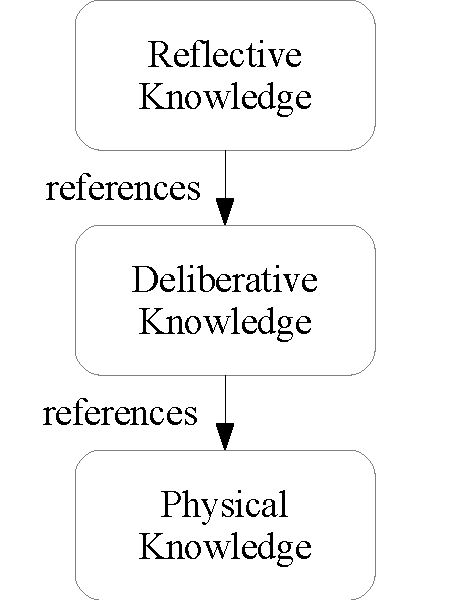
\includegraphics[width=4cm]{gfx/three_knowledge_layers}
  \caption{Three knowledge layers.}
  \label{figure:three_knowledge_layers}
\end{figure}

\section{Natural Language Plans}

SALS includes a simple but powerful planning language that is based on
the interpretation of natural language plans.  Plans are sequences of
commands that can be created, mutated, and executed by a planner in
order to accomplish goals.  The following is an example of a
definition of one of the deliberative plans that the AI in the story
could consider executing:
\begin{samepage}
\begin{Verbatim}
[defplan 'move slowly until over a cube'
  [plan-call [plan 'if a cube is to my left, move slowly
                    left until over a cube, otherwise if a
                    cube is to my right, move slowly right
                    until over a cube']]
  [plan-call [plan 'assert that a cube is below me']]]
\end{Verbatim}
\end{samepage}
This expression defines a new deliberative plan.  The ``defplan''
command is shorthand for ``define plan.''  The first argument to the
defplan expression is the name of the plan: ``move slowly until over a
cube.''  The body of the plan is the remaining sequence of
expressions.  The first expression in the body of this plan is to
interpret and execute the natural language phrase beginning with ``if
a cube...''  The second expression in the body of this plan is to
interpret and execute the natural language phrase beginning with
``assert that...''  This plan positions the AI over a cube and fails
if a cube is not finally below the AI.  If the planner wanted to find
a plan to position the AI over a pyramid, this plan would not help
unless it was slightly modified, replacing all mentions of ``cube''
with ``pyramid.''  In order to help the planner to know what parts of
plans might be analogously replaceable in this way, the SALS planning
language includes optional natural language pattern matching templates
and default frame variable bindings that can be specified for each
plan definition.  The following example shows how this simple plan can
be generalized to allow positioning the AI over a range of shapes:
\begin{samepage}
\begin{Verbatim}
[defplan 'move slowly until over a cube'
  :matches ['move slowly until over a [? shape]']
   :frame [[shape 'cube']]
    [plan-call [plan 'if a [? shape] is to my left, move
                      slowly left until over a [? shape],
                      otherwise if a [? shape] is to my
                      right, move slowly right until over
                      a [? shape]']]
    [plan-call [plan 'assert that a [? shape] is below me']]]
\end{Verbatim}
\end{samepage}
This generalized form of the original plan uses natural language
variables that are specified with a question mark expression, ``?''
Note that there are two optional arguments to the defplan expression
in this example: (1) ``:matches'' and (2) ``:frame.''  The optional
``:matches'' argument specifies a list of potential patterns that this
plan may match as it is being interpreted.  In this case, the variable
expression ``[? shape]'' is allowed to replace the word ``cube'' from
the original name of the plan.  The optional ``:frame'' argument
specifies the default natural language variable bindings.  In this
case, the ``shape'' variable is assigned the natural language phrase
``cube'' by default.  In the body of the generalized form of the plan,
all occurrences of cube have been replaced with the variable
expression ``[? shape]''.  Given this generalized form of the original
plan, the planner can create a new analogous plan as an interpretation
of the natural language phrase ``move slowly until over a pyramid.''
In this way, plans can be communicated to the AI in a natural language
form.  The AI has ``been told'' a total of approximately seventy
simple natural language plans, which can be adapted by analogy to
provide interpretations for a variety of complex possible natural
language plans, including recursive interpretations.  The details of
the planning language will be discussed in
{\mbox{\autoref{chapter:learning_from_being_told_natural_language_plans}}}.

\section{Layers of Learning}

SALS includes an efficient relational learning algorithm in each layer
of planned thinking.  Relational learning in SALS is handled
concurrently with the plan execution in that layer.  In this way, as
plans are executed at full speed, a trace of changes are produced and
sent to a parallel event consuming algorithm that induces abstract
partial states that are used to train a rule learning algorithm.  The
hypotheses that the rule learning algorithm creates are used to
provide explanations as to the parts of the plan that have caused the
traced changes.  I have found that the separation of learning and
planning into concurrent algorithms gives the learning algorithm the
time to work more slowly, while the plan execution can be performed in
bursts at near full speed.

The deliberative layer makes deliberative plans composed of physical
actions in order to accomplish deliberative goals, while the
reflective layer makes reflective plans composed of deliberative
actions in order to accomplish reflective goals.  Deliberative
learning allows the AI to better predict the physical effects of
deliberative plans for physical action, while reflective learning
allows the AI to better predict the deliberative effects of reflective
plans for deliberative action.  The AI is learning at a reflective
level when it thinks to itself, ``I also have new support for the
hypothesis that executing plans that try to accomplish the goal of a
cube being on a pyramid may lead to an expectation failure when
executed.''  This newly supported hypothesis is a reflective
hypothesis about deliberative actions and objects.  The AI
hierarchically assigns credit to the responsible parts of the
executing plan, ``find and execute a recently learned plan to
accomplish my goals,'' that was currently executing at the time of the
unexpected failure.  This precondition for the execution of the plan
is hypothesized to lead to the effects of this action in deliberative
knowledge, ``a deliberative planner is focused on a plan that has
failed.''  The next time that the reflective layer is deciding whether
or not the deliberative planner should execute a given plan, it can
consider this new knowledge and predict whether or not executing the
current plan will put the deliberative planner into a negative or
positive deliberative goal state.  I will discuss the details of SALS'
parallel relational learning algorithm in
{\mbox{\autoref{chapter:learning_asynchronously_from_experience}}}.

\section{Document Overview}

Each of the four contributions of this thesis will be discussed in one
of the following four chapters.  My implementation of the bottom four
layers of an Emotion Machine cognitive architecture is discussed next
in {\mbox{\autoref{chapter:emotion_machine_cognitive_architecture}}}.
In
{\mbox{\autoref{chapter:learning_from_being_told_natural_language_plans}}},
I will describe the natural language planning language that allows
natural language plans to ``be told'' to the AI.  This chapter will
also discuss how the planning process interprets natural language
plans by finding analogies to plans that the AI already knows.  In
{\mbox{\autoref{chapter:learning_asynchronously_from_experience}}}, I
will describe how the AI learns from the experience it gains from
actually executing its plans.  This chapter will describe the
necessary procedurally reflective components that have been used to
attach complex time-intensive learning algorithms to quickly executing
plans of action.  In order to describe my last contribution, I will
describe the SALS virtual machine and reflectively traced programming
language in
{\mbox{\autoref{chapter:virtual_machine_and_programming_language}}}.

{\mbox{\autoref{chapter:related_models}}} relates my AI to other
contemporary cognitive architectures, approaches to reflective
thinking, metacognition, and learning to plan, as well as other
massively multithreaded computer systems.
{\mbox{\autoref{chapter:evaluation}}} evaluates the run-time
performance of the SALS AI and shows a sub-linear increase in
time-complexity for each additional reflective layer.  In
{\mbox{\autoref{chapter:future}}}, I discuss promising directions of
future research for extending this architecture to learn at the top
two layers of the Emotion Machine theory, the self-reflective and
self-conscious layers.  Also, in this chapter I discuss approaches to
overcoming some of the current limitations in the SALS cognitive
architecture.


\cleardoublepage\part{The Model}\label{part:the_model}
%************************************************
\chapter{The Dynamic and the Static}
\label{chapter:the_dynamic_and_the_static}
%************************************************

In this dissertation the focus will be a description of thinking that
reflectively learns to accomplish goals.  I begin by describing a
clear distinction between the dynamic and the static, which is
\emph{the} fundamental key distinction in my model.  The model of
reflective thinking grows quickly within this initial foundational
conception, which, as it begins reflectively, leads necessarily and
naturally to the goals of this dissertation.  This part will give a
non-technical understanding of my reflective model of mind, which is
the basis of the mathematical simulation and the computational
implementation.

I will not attempt to give a complete representation for a general
problem domain nor a complete description of a general problem solver.
My work here leaves the unmodellable as known to be just that.
Thinking as a dynamic activity uses models as useful tools with the
clear understanding that these models are static.  Further, and
critically important for the advancement of the field of AI, when
describing reflective thinking, it is imperative to have an explicit
awareness of thinking being limited to manipulating the static.  I
will therefore refer to an AI model as simply an ``AI'' with the
shared understanding that I am referring to a static model.

Non-reflective AI models learn by correcting one immediate cause of a
failure; however, given a layered model, I describe new opportunities
for considering one failure to also be failures in the reflective
layers ``above'' and ``below'' the original failure, resulting in an
arbitrary number of reflective learning opportunities from a single
failure.

In \autoref{part:the_simulation}, the simulation, I will describe an
example of a mathematical description of the model, which I will use
to evaluate the model in terms of the performance of a search
algorithm implemented in a reflective simulation.

In \autoref{part:the_implementation}, the implementation, I will
describe an example of a computational implementation of reflective
thinking.  The implementation is a layered cognitive architecture with
three working layers.  I will focus on a very simple physical block
stacking problem domain as a tool for explaining simply, through
examples, the layered classes of reflective learning.  In describing
the working model implementation, I will maintain an awareness of the
explicit distinction between a static model and the dynamic referent.
I have categorized my focus in this way only as an example of the
computational description.

\section{Dynamically Grounded Description}

A grounded description references the dynamic.  Symbols, words and
language, have grounding only in this way.  The further ability of
symbols to also reference other symbols allows the additional
possibility of creating a referential circularity in the static model.
An illusion of a primitive grounding is possible in such a cycle
because all of the symbols have a referent; however, because all
references within such a closed cycle appear to be exclusively kept
within the static model and do not seem any longer to refer to
anything dynamic, there is a danger of there being no meaning other
than circularity to such a purely static construct.  Again, symbols
are tools for modelling and are useful only if the circularity is not
mistaken for a grounded reference.  Thus, I strictly avoid presenting
such illusions of grounding as primitive in this dissertation.  To
allow for grounded descriptions, I will first outline my conception of
the dynamic, to which my description ultimately must refer.  A
description of reflective thinking referring to an \emph{a~priori}
concept that has not been derived in terms of symbols allows for
something to remain outside of the static model as the dynamic
referent.  This last step avoids the creation of a purely
self-referential cycle and prevents illusions from becoming mistaken
for grounded parts of the model.  In the next section I will describe
the necessary conception of the dynamic to which my description of
reflective thinking will refer.

\section{Activities in Duration}

\cite{bergson:1910}, in his seminal \underline{Time and Free Will},
discusses the dynamic as heterogeneous activities in Duration.
Activities in Duration will serve as my conception of the dynamic for
my description of reflective thinking.  Activities in Duration are the
dynamic ongoing activity, heterogeneous activities that are neither
distinct nor separate.  There is a trick, a sort of slight of hand,
required here in describing Bergson's conception of the activities in
Duration because, even though referred to through symbolization, these
activities exist independently of symbolization.

For example, when I look at a tree, I may say that the tree has green
leaves and a brown trunk; the symbols, green and brown, refer to the
activities in Duration, which I am seeing.  When I focus carefully on
the dynamic activity of my situation, I see that the leaves and trunk
could be described by a greater combination of various greens,
yellows, grays, browns and reds.  Symbols limit perception to a
discrete sort of projective presupposition.  Therefore, as I introduce
more symbolic references in my increasingly limited description of the
dynamic, a growing danger of losing focus on something dynamic
emerges, creating a cycle of symbols seemingly referring exclusively
to symbols.

The motivation to tangentially define more clearly what I mean by the
symbol green or brown by using more symbols results in a circularity
from which there is no exit, and therefore, a false dilemma from which
I will never again be able to see or talk about any dynamic tree as
the referent.  In order to avoid the danger of purely cyclic symbolic
references in my model, I will continue to relate the parts of my
model to the dynamic activity of reflective thinking, which exists as
activities in Duration.

\section{Actual Reflection}

The activities in Duration are the given dynamic ongoing.  These
activities are the inseparable actions that are currently available to
reflection.  Reflection is the ability to symbolize this ongoing
activity.  For example, the activity of perceiving a table can be
symbolized as the name ``table''.  Similarly, the activity of walking,
can be symbolized as present participle ``walking''.  Note that my
model of reflective thinking assumes that there is ongoing activity
before any symbols exist for the actions of thinking to manipulate.
Thinking is an auxiliary activity that manipulates static symbolic
constructions that refer to the primary ongoing activity of existence.
Thus, the activity of perceiving a table requires neither that this
activity itself be reflectively symbolized nor that a secondary
thinking activity manipulates the resulting symbols.  I will use the
phrase \emph{actual reflection} to refer to the activity of
symbolizing ongoing activities.

\section{Order of Space}

Activities in Duration may be symbolized in a homogeneous medium
without activity.  Bergson calls this medium Space, allowing symbolic
references to activities in Duration to be related.  This is the
primary fundamental distinction in both the mathematical simulation
and computer implementation of reflective thinking.  Of major
importance is the fact that one does not derive the other, but
activity and order coexist with neither Duration being a derivative of
Space nor Space containing the fundamental activities in Duration.
Obviously, Bergson has gone through painstaking efforts to leave room
in his description for the dynamic as some independent, non-contingent
activity not derived from either Space or Duration.  He makes the
necessary concession that a description of something dynamic is only
grounded in that it leaves room for this dynamic to exist
independently of its own symbolization.  This modelling work is meant
to be similarly grounded in the necessarily separate dynamic activity
of reflectively learning to accomplish goals.

\section{Modelling the Dynamic}
\label{section:modelling_the_dynamic}

Duration and Space are the fundamental duality that forms the basis of
my model of the dynamic activity of reflectively thinking.  Thus this
duality exists pre-reflectively, prior to symbols being created from
the activities in Duration and prior to these symbolic references
being related in Space.  Note the fundamental contradiction of
intentionally describing the dynamic only in static symbolic terms.
For example, if Space has no activity and is not itself composed of
activities in Duration, to what is the symbol ``Space'' referring?
Symbol ``Space'' refers only to the logical potential for an absence
of activity, the potential for itself as not existing; thus, it is the
logical necessity of the negative implication of positive existence,
to which no alternative can be assigned.  Again, my model explicitly
does not provide a definition of this implicit, fundamental and
irresolvable contradiction.  Thus, my description will appear to begin
in the middle of something endlessly dynamic and ongoing, the \emph{in
  medias res} of an underived time and space, maintaining an explicit
awareness that static descriptions are only tools for dynamic
reflections.  Duration and Space are not placeholders for the dynamic;
they are intermediate programmed fictions in the implementation that I
use here to model the dynamic ongoing, the actual activity, which is
not a static arrangement of symbols.

\section{Spatial Reflection}

The activities in Duration are the dynamic activity of being in the
present.  Symbols, like the photographic, are static references to
this dynamic.  Again, there is a fundamental distinction here between
the dynamic and the static.  Because AI already refers to an AI model,
I use an asterisk notation to refer a model that the AI learns in
simulation.  In this way, Spatial arrangements of symbols can actually
exist in the dynamic as an actively maintained static construction, a
model* within the AI.  The ongoing activities that hold symbols in a
specific Spatial arrangement can be symbolically reified.  I will
refer to the activity of symbolizing the activities of a Spatial
arrangement of symbols as \emph{Spatial reflection} or
\emph{reification}.  Spatial reflection is a form of actual
reflection.

\section{The Physical Layer}

My model includes three layers of ongoing dynamic activity.  I will
use the phrase \emph{physical layer} to refer to the pre-reflective
layer of activities that exist necessarily prior to any subsequent
reflective symbolization activity.  The physical layer is the only
pre-reflective layer of activity in my model.  Therefore, a clear line
is drawn between the physical layer and those activities that
symbolize and Spatially arrange symbols.  Thus, they are not included
in what I will refer to as physical activity.  Note that in most AI
models, there is a distinction between the mind and the body or the
environment.  In my model, \emph{all} activities that exist are
referred to as \emph{the mind}.
\footnote{Because my model of mind is an absolute reference to the
  dynamic, it makes very few modelling assumptions.  Because my model
  has been previously mistaken for the philosophy of ``Subjective
  Idealism'', I have included a description of the mistake of
  Subjective Idealism, and a clarification that my model does not make
  this mistake, an important difference between my model and this
  problematic philosophy; I explain in
  \autoref{section:the_mistake_of_subjective_idealism}.}  Thus, the
dynamic mental activities that I am referring to in my model are not
an object that is viewed subjectively.  Critical to an understanding
of the goals of objective science is that the creation of object and
subject distinctions is allowed to be a part of the activities of the
mind that can be simulated with my AI; because this understanding is
so critical to an advancement of scientific understanding, I will
clarify the mental derivation of objective science in
\autoref{chapter:science}.  Because the abstract creation of object
and subject relationships is a relatively advanced mental activity and
not key to my thesis, I will discuss this as future research in
\autoref{chapter:future}, which would be a promising place to extend
my model to include ideas like physical bodies and other subjective
and objective environmental perspectives.

\section{Orders of Reflective Layers}

In addition to the pre-reflective physical layer of activity, my model
includes two additional layers of reflective thinking activity that
use two different classes of causal models in order to accomplish two
different classes of goals.  I will use the phrase \emph{first-order
  reflective layer} to refer to the reflective layer of thinking that
creates symbols and Spatial arrangements that refer to physical
activities.  I will refer to reflectively symbolizing physical
activities as \emph{physical reflection}.  Physical reflection is a
form of actual reflection and is one of the primary reflective
thinking activities; remember that physical activities are
pre-reflective, so physical reflection is not itself a physical
activity.

Obviously, the first-order reflective layer cannot create symbols or
Spatial arrangements that refer to its own activities, with one
obvious exception: Spatial reflection, as already mentioned.  The
first-order reflective layer has the \emph{a~priori} ability to
maintain its own actively reified Spatial relationships as existing
between symbols that refer to physical activities.  The lack of the
ability for the first-order reflective layer to refer to its own
symbolically creative or Spatially manipulative activities acts as a
sort of protective ``firewall'' that clarifies my model by keeping
clear distinctions between each class of causal knowledge in each
subsequent reflective layer of thinking.  Before describing
distinctions between classes of causal models, I will spend the next
few sections describing the composition of temporal transitions and
causal hypotheses.

Reflection over the activity of the first-order reflective layer
necessarily creates a second layer of reflection and thinking.  Thus,
clearly deriving and describing this second layer of reflective
thinking additionally necessitates an implicit and arbitrary number of
layers.  This condition is the focus of this dissertation.
\cite{minsky:2006} describes a six-layer reflective model of thinking
about thinking.  The first three layers of my model and
implementation, including these two layers of reflective thinking, can
be compared to the first four layers of Minsky's model.  There are
many close parallels between my model and Minsky's model, and I will
describe these modelling parallels in
\autoref{chapter:related_models}.

\section{Consciousness, Awareness, and Experience}

There are many terms that are used in the literature when referring to
the concept of the dynamic.  Each of these terms has a different
associated collection of necessary contingencies that, as isolated and
independent, tend to become absurdities.  For example, the general
term consciousness always begs the question \emph{of what} one is
specifically conscious.  There is an implicit independence of subject
and object when using this transitive term, which is not assumed when
the term is used as a reference to the dynamic.

The terms awareness and experience are used similarly and have the
same logical contradictions as the term consciousness when they are
considered as independent isolated references to the dynamic.  Each of
these terms has different meaningful uses when they are not used in
this independent sense.  For example, in this dissertation an
awareness of the potential confusions these terms introduce when they
are used singularly in abstract isolation as reference to the dynamic
will be maintained.

Thus, I will not argue that these conceptions of the dynamic are
incorrect.  Rather, they are limited to particular and less
generalized models that are restricted descriptions of the dynamic.
In this dissertation, however, in order to avoid confusion, I will
never use these terms in their limited and abstracted sense.  Instead,
I will conflate all of these uses of these terms as all being the same
as my conception of the dynamic, the ongoing activity that my model
accepts, symbolizes, and thinks about as given.

\section{Extensive and Intensive Quantities}
\label{section:extensive_and_intensive_quantities}

Sometimes it is hard to imagine how a fundamentally symbolic model can
ever refer to the ``intensities'' of perceptual stimuli.  Thus, in
this section, I make a distinction between two types of intensities,
the ``extensive'' and the ``intensive''.  This distinction is used to
explain how the basic symbolic component of the model can come to
represent various aspects of everyday thinking that, according to
common sense, are fundamentally of a certain intensity.

\cite{bergson:1910} makes a key distinction between comparisons of
``extensive'' quantities and comparisons of ``intensive'' quantities.
Extensive quantities are Spatial comparisons.  \emph{Extensive
  quantities} are between two symbolic references that share a
containment relationship in terms of their referents: one symbolic
referent is inclusively contained by another symbolic referent in
Space.  For example, one body may be said to be larger than another in
terms of its Spatial extent.  Intensive quantities are more subtle and
an example is in terms of pain, which can be said to be more or less
intense.  \emph{Intensive quantities} are similar to neither
numerically nor Spatially extensive containment relationships but,
instead, refer to different fundamental activities in Duration.  For
example, a pain that has no intensity is not a pain at all; a pain
that has a mild intensity may be equivalently referred to as an
irritation or an itch; a pain of high intensity may be equivalently
referred to as a sharp pain or a throbbing pain.  The point is that
these intensities of quality are actually very different from
extensive quantities in that they are not greater than or less than
one another in the sense of a containment relationship.  For example,
a very intense pain, such as a shooting pain or a throbbing pain, does
not in any sense contain a lesser mild pain, such as an irritation or
an itch.  This same pattern exists with detailed descriptions of other
qualities that are often thought of as having comparable intensities:
heat and cold; light; pressure; sound; pitch; aesthetic feelings, such
as grace and beauty in music, poetry and art; emotions, such as rage
and fear; moral feelings, such as pity; affective sensations,
including pleasure, pain and disgust.  Each of these examples points
out that the apparent relationships of greater than or less than with
respect to intensity are static Spatial arrangements of different
fundamental activities in Duration.

\section{Number}
\label{section:number}

Some models make the complicating assumption that numbers are an
additional component to every symbolic perception just for this
purpose of modelling intensity.  In this section, I describe how
numbers are related to the model: numbers are thought of in my model
as arrangements of symbols in Space.

\cite{bergson:1910} shows the derivation of all numerical
representations as requiring an accompanying extension in Space.  For
example, in referring to the individual sheep in a flock of sheep, he
explains counting:

% pg. 75-77
\begin{quote}
Number may be defined in general as a collection of units, or,
speaking more exactly, as the synthesis of the one and the
many\ldots

No doubt we can count the sheep in a flock and say that there are
fifty, although they are all different from one another and are easily
recognized by the shepherd: but the reason is that we agree in that
case to neglect their individual differences and to take into account
only what they have in common.  On the other hand, as soon as we fix
our attention on the particular features of objects or individuals, we
can of course make an enumeration of them, but not a total\ldots

Hence we may conclude that the idea of number implies the simple
intuition of a multiplicity of parts or units, which are absolutely
alike.

And yet they must be somehow distinct from one another, since
otherwise they would merge into a single unit.  Let us assume that all
the sheep in the flock are identical; they differ at least by the
position which they occupy in space, otherwise they would not form a
flock.
\end{quote}

The last point here illustrates the idea that numbers are always
derived from symbols situated in Space.  Therefore, a model for
thinking based directly on symbols cannot, by definition, be more
complicated than a model based on a numerical representation.  A
number is, after all, only the reified result of an axiomatic
construction of Spatial organization of symbolic references to the
dynamic.  In other words, they are specific sheep of the dynamic.  The
explicit implication is, therefore, that, in building an AI that is
capable of reflective thought, the model building process and its use
of numerical representations must be explicitly available for
inspection by the AI itself.  Here, I employ Occam's razor to simplify
the loop of reflective representation in order to ease building the
first proof-of-concept examples of AIs capable of reflective thinking.

\section{Time as Space}

Symbolic references can be ordered Spatially.  These symbolic
relationships can be reified and treated symbolically by further
ordering Spatial relationships.  Thus, Bergson explains time as a form
of Space:

% pg. 98
\begin{quote}
Now, if space is to be defined as the homogeneous, it seems that
inversely every homogeneous and unbounded medium will be space.  For,
homogeneity here consisting in the absence of every activity, it is
hard to see how two forms of the homogeneous could be distinguished
from one another.  Nevertheless it is generally agreed to regard time
as an unbounded medium, different from space but homogeneous like the
latter: the homogeneous is thus supposed to take two forms, according
as its contents co-exist or follow one another.  It is true that, when
we make time a homogeneous medium in which conscious states unfold
themselves, we take it to be given all at once, which amounts to
saying that we abstract it from duration.  This simple consideration
ought to warn us that we are thus unwittingly falling back upon space,
and really giving up time.
\end{quote}

Time exists as a static creation, a derivative arrangement of symbols
in Space.  Understanding time to be static is important because this
allows the dynamic heterogeneous activities of Duration and a static
homogeneous unqualified Space to remain, respectfully, neither
distinct nor separate.  By prohibiting this separation, and, thereby,
their independent existences, I avoid defining the dynamic activities
in Duration in terms of static symbols, which, in turn, avoids the
creation of a self-referential cycle, thus sidestepping the potential
illusion of a false dynamism.  Being clear in our understanding of
time used intentionally as a static tool of thought avoids confusing
the focus of the modelling process to focus on modelling the dynamic.
Again, a model that is purely of a model leads to an AI based on a
tautology because models are only grounded in that they reference the
dynamic.

\section{Temporal Reflection}

Spatial arrangements of symbols can be used to represent a past
through memory and subsequently project that distinction as an
analogous ``future'', through imaginative action, thus constructing a
derivative conception of time.  The past and the future, therefore,
remain static constructions that are actively maintained by the model
as Spatial relationships in the dynamic present.  I will refer to the
reification of Spatial relationships that order the past and the
future as \emph{temporal reflection}.  Sequential time is created
through temporal reflection.  Thus, temporal reflection is a form of
Spatial reflection.  Like Spatial reflection, temporal reflection is
also a form of actual reflection, symbolizing the active maintenance
of a temporal Spatial relationship between static symbolic references.

\section{Simultaneity and Transition}

Correlation requires two symbols to be related in Space.  As symbols
are correlated in the Space called time, these temporal correlations
are referred to as either simultaneities or transitions.
Simultaneities represent two symbols that are both actively symbolized
in Duration.  Transitions represent the change from the past to the
future.  Transitions can be extended in time in order to create
counterfactual temporal extensions, called inferences.  Inferences of
the past and the future can be created by matching and repeating these
transitions.  A transition implies the removal of one symbol and the
addition of another as a progression is made through a temporal
sequence.  If correlations are counted and compared in ratios, then
these are called probabilistic correlations, and the resulting
inference would be a probabilistic inference.


%************************************************
\chapter{Learning Causal Hypotheses}
\label{chapter:learning_causal_hypotheses}
%************************************************

\section{Resources}

Activities in Duration can be referred to symbolically by the
reflective thinking layers.  While all activities in all layers are
qualities of Duration, these activities can be symbolized as
potentially actionable parts of plans by the reflective thinking
layers.  I will refer to a symbolic reference to activities that can
be put into plans as a \emph{resource}.  Resources exist in the
thinking layers as symbolic references to activities in the layers
below.

\section{Activation and Suppression}

In my model, I've included a logical idea that I refer to as
\emph{suppression}.  Suppression is a symbolic relationship to a
resource that can be put into plans.  The idea of suppression is a
subtle point with respect to the qualities of Duration.  The basic
problem is that the qualities of Duration are the activities that
exist independently without thinking existing as any implicit,
co-existent necessity.  Further, the activities in Duration cannot be
inactive, by definition.  This is important.  In other words, a
symbolic reference to something inactive would imply a symbol that
refers to something that does not exist, or, in other words, only
exist as a contradiction.  Therefore, the logical idea of suppression
is only an artificial tool of thought, part of the thinking layers,
entirely separate from physical activities.  The subtle point here is
that suppression does not disable the potential for activities.
Suppression is only a logical Spatial relationship including the
symbolic reference to the physical activity in question.  I will refer
to the logical alternative to suppression as \emph{activation}.
Activation and suppression refer to types of assumed Spatial
relationships that are maintained between symbolic resources.
Therefore, it would not be correct to say that physical activities
have been activated or suppressed, but alternatively, it would be
correct to say that a resource is in an ongoing, unstoppable, dynamic
Spatial relationship that has activated or suppressed qualities.  The
activation and suppression of resources occurs in the sense of
actively creating Spatial relationships that represent the logical
qualities of activation or suppression, which have the potential to be
logically consistent or contradictory.

Therefore, in my model, a resource can be both either activated or
suppressed, which does not, by itself, imply a resultant activity in
the layer below; logically, if a resource is activated and is not
otherwise suppressed, then the resource is considered logically to be
activated; however, when a resource is both activated and suppressed
simultaneously, this is a logical failure that is cause for a plan to
halt execution.  Before discussing potential responses to plans
failing in this way, it will obviously be necessary to first discuss
the basics of the planning process.

\section{Cause and Effect}

Two symbols correlated in time are not enough to compose a causal
relationship.  Two symbols correlated in time are simply a coincident
transition from the past to the future.  A causal relationship
supposes an additional component, a necessary connective symbolic
reference to the activities that are ongoing during the transition.
Thus, the effect of the causal component becomes the transition
itself.  A causal relationship, therefore, has three parts: the
symbolized qualities of Duration active in the present, the symbolized
qualities of Duration in the past, and the symbolized qualities of
Duration in the future.  I will sometimes refer to these three parts
of the causal relationship more succinctly as (1) the cause, (2) the
necessity, and (3) the result.  When causal models are used for
planning, the symbolic reference that is the cause is referred to as a
resource.

\section{Goal Activities}

It is important to understand that, in my model, goals are not
derivatives of symbolized perceptions.  Symbolized goals refer to the
fundamental activities in Duration that give \emph{a priori} direction
to the activities of thinking.  Goals can thus be arranged in Spatial
orders, according to preferential qualities; i.e. goals can be
considered to be positive or negative, something to seek or something
to avoid.

In my model, a goal is simply a reference to these activities that
symbolically exist in Duration.  Qualities of Duration can symbolized
as goals, remaining generalized without becoming anything specific or
fundamental in themselves.

The first-order reflective layer symbolizes goals and this creation of
a symbolic reference to goal activities becomes the reason for
planning and acting toward or away from the associated perceptions.
Note that because symbolic goals, perceptions, and resources in my
model are artificial and do not derive from one another, a process of
refining symbolic references to perceptions and resources can be
undertaken in the pursuit of creating more accurate causal models that
predict the activities in Duration that symbolic goals reference.

\section{Causal Hypothesis}

When goal activities are symbolized, causal hypotheses can be created
for predicting the goal activities in the future.  For example, if
there are ongoing activities happening simultaneously with the
symbolization of the goal, these can be hypothesized as causes of a
future symbolized goal.  Remember that a causal model has three parts:
present cause, past, and future.  In this case, the goal is placed in
a future context, the symbolized current activity is in the present,
and there must also be a past symbol to fill the last slot in the
model.

\section{Limitations of Logical Goals}

Logical approaches to AI have seen the value in considering goals to
be relative arrangements of perceptual symbols.  These sorts of
symbolic relationships in my model are thought of as occurring
simultaneously with, before or after goal activities.  Artificial
constructions that are actively maintained in Spatial arrangement can
be reified as symbolic perceptions, but fundamentally the goal does
not refer to an artificial construction, despite the possible
correlation of goals with such constructions.  In this way, my model
gains the ability to think about and refine the symbolization of
perceptions because symbolic goals refer to the actual qualities of
Duration, instead of the inversely limiting assumption that goals are
specified in terms of artificial constructions of perceptual symbols.
Artificial constructions are useful tools for accomplishing goal
activities; however, reflectively, all artificial constructions,
including symbols, are caused by the AI itself and the correspondingly
responsible activities can change.  Thus, all symbolic constructions
are explicitly available as artificial references that are available
for inspection by the AI itself.  In other words, in purely logical
approaches to AI, symbols are not understood to be artificial
creations of the AI itself and, thus, cannot be reflectively debugged
when they are wrong.

In order to allow these logical approaches to adapt, I see no
alternative but to fundamentally reinvent all logical approaches to
problem solving in reflective terms that acknowledge a dynamic reality
and the static artificiality of symbols, allowing the potential for
debugging meaningful and useful symbolic constructions.  AI systems
must use symbols in full awareness of their creation as pliable
artificially static references to a dynamic unstated actual existence.

\section{Physical Goals}

The primary class of goals that can be symbolized is called the
physical goal.  Physical goals refer to dynamic activities in Duration
that are the cause for refinement and initial creation of static
symbolic perceptions and resources.  These initial symbolic
perceptions and resources are thus physical as well.  The primary and
most fundamental class of causal hypothesis is the physical causal
hypothesis, composed of physical perceptions, resources, and goals.
All of this initial knowledge stems from the most fundamental class of
goal, the physical goal.

\section{Reflective Classes of Causal Models}

The first-order reflective layer creates causal models from physical
perceptions, resources, and goals.  I've described previously how
goals can cause reflective thinking to create causal hypotheses.
Another way to state this more succinctly is as follows: \emph{goals
  are the cause of causal hypotheses}.  Note two different meanings of
cause in the previous sentence.  In the latter case, I'm referring to
causal models relating physical perceptions and resources, and in the
former case, I'm referring to the first-order reflective activity that
causes the creation of the physical model.

Allowing activities of the first-order reflection to be available for
inspection by the AI itself allows my model to represent the
transitions caused by first-order reflective activities.  These
transitions are knowledge level changes.  By using this reflective
technique, a new class of causal model is created, categorically
different from the physical causal models that the first-order
reflective layer manipulates.  When the activities of the first-order
reflective layer are reflectively symbolized, my model can then be
motivated to learn to accomplish or avoid knowledge level goals, using
knowledge level causal hypotheses.

\section{Probabilistic Causal Models}

Probabilistic models are an advanced and important thinking tool.
Building a probabilistic causal model involves counting symbolic
perceptions, resources, and goals.  For example, let us consider that
two causal hypotheses have been created that reference the same
symbolic cause and the same symbolic perception in the past; let us
say that the only difference between these two hypotheses is that they
refer to two different symbolic goals in the future.  This situation
gives my model a reason to further distinguish symbolic
representations for perceptions and resources, introducing more
refined symbols for these perceptions and resources in order to lead
to causal models that are more useful for correctly predicting these
two different symbolic goals.  This would be the more appropriate
course of action if we wanted to correctly predict the symbolic goals;
however, there is an opportunity here to build a probabilistic model
that does not refine the symbolization of perceptions or resources.
For example, both of the two causal hypotheses could be considered
together to compose a probabilistic causal hypothesis.  Using this
probabilistic hypothesis, a future inference could be created that
includes both symbolic goals, each with one half of a potential
existence.  Probabilistic causal hypotheses are useful for predicting
the average number of times that a symbolic event will occur.  Note
that probabilistic causal hypotheses require counting and creating
ratios from the more fundamental non-probabilistic causal hypotheses
from which they are constructed.


%************************************************
\chapter{Layers of Reflective Thinking}
\label{chapter:layers_of_reflective_thinking}
%************************************************

\section{First-order Reflective Thinking}

After constructing causal hypotheses that predict the necessities and
results of activating resources, these causal models are used to
construct larger structures called plans.  Plans are combinations of
causal models that contain inferences of past necessities and future
results.  For example, one could imagine a sequence of resources that
leads through a counterfactual future sequence of perceptions,
resources, and goals.  In the literature, these counterfactual
constructions are referred to by a number of names, including: case,
explanation, fiction, narrative, and story.  Stories and narratives
often include a social self-reflective representation, which I see as
future work in the development of my model, which I will discuss in
\autoref{chapter:future}.  I will simply use the term plan to refer to
all of these constructions that combine causal models into
counterfactual views of the past and future.

First-order reflective thinking is the ongoing activity in Duration
that is limited to manipulating symbolic references to physical
activities.  First-order reflective thinking symbolizes physical
activities, creates physical causal hypotheses, and uses these
hypotheses to create plans toward or away from physical goals.
Further, first-order reflective thinking activities execute these
plans composed of physical resource causal symbolic references.

\section{$n^\text{th}$-Order Reflective Thinking}

I've previously described three layers of activity in my model: the
physical layer, the first-order reflective thinking layer, and the
second-order reflective thinking layer.  For brevity, and to emphasize
the layered nature of my model, I will sometimes use a superscript
notation ``$\text{reflective}^n$'' to refer to the $n^\text{th}$-order
of a layer in my model.  For example, the $\text{reflective}^1$ layer
will refer to first-order reflective activities, and the
$\text{reflective}^2$ layer will refer to second-order reflective
activities.  Although the physical layer is not a reflective thinking
layer at all, its place as the prior reference for the first-order
reflective thinking activities moves me to inductively extend this
notation to allow referring to the physical layer as the
$\text{reflective}^0$ layer or the \emph{zeroth-order reflective
  layer}.  Zero thus becomes the origin of an infinite regress of $n$
layers.  In this sense, the implementation of my model of reflective
thinking includes activities of reflective order zero through
reflective order two.

\section{Limitations of First-order Reflective Thinking}

The act of creating a symbolic reference to physical activity is not
accessible to the first-order reflective layer; it is critical to
understand this.  A creative first-order reflective layer action, such
as creating a plan toward a physical goal, is limited to creating and
Spatially arranging symbols that refer to physical activities.  The
first-order reflective layer does not manipulate symbols that refer to
its own activities without reducing itself to something meaninglessly
tautological.

Another critical point to understand is that first-order reflective
thinking does not directly manipulate physical activities.  Neither
symbols nor Space are physically actual; instead, symbolic references
to physical activity and the relationships that order them in Space
are artificial creations of an independent first-order reflective
layer.  First-order thinking is about physical activities and is
limited to the terms of its own willfully created artificial symbolic
references to the actual physical layer.  In contrast, the physical
layer does not include any of the artificial constructions of
thinking, neither symbols nor Spatial arrangements.  This is because
the physical layer does not include thinking, which is fundamentally a
reflective activity.

\section{Second-order Reflection on Symbolization}

First-order reflective thinking activities create, Spatially arrange,
and otherwise manipulate symbolic references to physical activities.
The activity of symbolization is a primary aspect of every reflective
thinking layer; however, given the logical limitation that reflective
thinking layers do not refer to their own activities with the
exception of active Spatial arrangements, a second-order reflective
thinking layer is necessarily required for creating symbolic
references to the activity of symbolization.  Note that the activity
of reflecting on symbolization appears in all layers above the
first-order reflective thinking layer, but this activity of reflecting
on the activity of symbolization necessarily first appears only in the
second-order reflective thinking layer.

\section{Non-existence of Symbolic References}

Reflecting on symbolization is one the primary activities of the
second-order reflective layer, resulting in the primary second-order
symbols that refer only retrospectively to first-order activity.
Having a symbolic reference to first-order symbolization allows
considering this activity to be symbolized as a second-order resource.
Considering first-order symbolization as a second-order resource thus
allows a second-order causal hypothesis to be created with this
resource as the ongoing cause of a transition.  In this case, the
transition is from the ``non-existence'' to the purely retrospective
existence of the first-order symbolic reference to physical activity.

Note that non-existence is a logical placeholder in the causal model,
which only refers to the logical alternative to willful creation and
existence itself.  I've begun my description with the assumption that
what exists is my reference, and that what exists does not require
symbols to refer to itself or describe itself.  However, in reflecting
on and symbolizing the activity of symbolization, I have implicitly
assumed this placeholder, ``non-existence'', in the causal model that
allows second-order reflective thinking about the existence of
first-order symbolic references.  Non-existence refers to the past
slot in the second-order causal model of first-order symbolization.
Causal hypotheses and their symbolic parts are artificial
constructions, so non-existence can only be a reference to part of an
artificial construction.  Non-existence is a modelling tool for
second-order reflective thinking.  Non-existence does not refer to a
primary quality of Duration, non-existence refers to an artificial
Spatial arrangement of symbols in the second-order reflective layer.

\section{Planning Symbolic Refinement}

There is a very useful opportunity here to extend the causal model
further into the past and predict the creation of new symbols based on
previous symbolized perceptions or resources.  This could lead to
second-order reflective thinking creating plans for the first-order
thinking layer to create new and more refined symbols that may be
useful for either accomplishing or avoiding physical goals.  This is a
useful and powerful type of second-order reflective planning.

\section{The Distractive Nature of Non-existence}

Non-existence as a tool of thought is as dangerous as it is powerful.
The danger is that non-existence can be incorrectly considered to be
\emph{the preexisting reality}.  In my model, I have defined reality
to be everything that exists as ongoing in Duration, maintaining an
awareness of the absurdity of describing something that is prior to
symbols.  Said another way, the danger is in forgetting that
non-existence is a reference to the past slot in an artificial causal
construction of at least order two.  This danger of mistaking
non-existence for the prior reality is insidious, distracting, and
tempting because of its false promise of an explanation for creation
and existence itself.

For example, the first-order reflective layer can create the
perceptual symbol ``green'' to refer the current undescribed physical
activities in Duration.  These ongoing physical activities do not
contain symbols and I have been very careful to not attempt to provide
a description of that which cannot be defined in terms of artificial
symbols, the activities ongoing in Duration, which are neither
artificial nor in artificial terms.  Therefore, the symbol ``green''
is an artificial creation that refers to these undefined activities,
which are the given qualities of Duration.  They require neither
symbolization nor thinking to exist.

Now, a second-order reflective thinking activity can create a causal
model of this first-order symbolization, the creation of the symbol
``green''.  This second-order activity implies that before the
creation of the symbol ``green'' there was a non-existence of the
symbol ``green''.  The problem is that the non-existence of the symbol
is actually the result of the creation of the symbol, so we must not
be confused when the second-order causal model places the
non-existence of the symbol in the past slot.  Non-existence of the
symbol is an artificial tool of thought.  ``Active non-existence'' is
just as absurd as ``inactive existence''; actual non-existence is a
tempting but simple contradiction.

\section{Third-order Reflection on Existence}

The second-order reflective layer creates causal models of the
creation of symbolic references.  These second-order artificial
constructions contain the primary references to existence and
non-existence.  Although my implementation does not include a
third-order reflective layer, my model includes the potential for an
arbitrary number of layers.  In order to briefly describe the
potential for third-order reflective thinking, let us consider a
causal model that would be the creation of the third-order reflective
layer.

For example, let the second-order activity of creating a causal
hypothesis be symbolized as a symbolic resource in the third-order
reflective layer.  This symbolic resource could refer to the
second-order creation of a causal hypothesis describing the
first-order creation of a symbolic reference to physical activity.  In
the past slot of this third-order causal model is the symbolic
resource that refers to the first-order creation of the symbol.  In
the future slot of this third-order causal model is a symbolic
resource that refers to the second-order creation of the causal model
that introduces the concept of existence being created out of
non-existence.  Note that the power of third-order reflection allows
the creation of the causal hypothesis that correctly places the
creation of the symbol prior to the simultaneous creation of the
knowledge of the existence and non-existence of the symbol.

\section{``Sub-symbolic Thinking''}

I have previously discussed the danger of having the second-order
reflective ability to create a causal model that predicts the
existence of symbolic perceptions from non-existence.  The danger is
in believing that the non-existence of a symbolic perception
represents some kind of pre-reflective mechanism that produces
symbols.  There is no such thing as a pre-reflective symbol or model.
Reflection creates symbols and models that refer to reality.  It is
important to understand that a causal model that predicts the creation
of symbols is the result of a second-order reflective activity, more
abstract and artificial than the first-order creation of the symbol.
Now, there have been many causal models that have been developed to
describe the creation of perceptual symbols.  Many of these are based
on the artificial extension of physically objective assumptions that
allow one to dissect brains and build models of perceptions based on
neural networks.  These neural network models are sometimes said to be
``sub-symbolic''.  It is important to realize that the integration is
illusive, that the idea of a model being sub-symbolic is a
contradiction in terms because all models are built from symbols.
These so called sub-symbolic models are actually at least at the level
of second-order reflection, which is the first level of reflection
that is able to model the creation of a symbolic perception.  I think
that referring to the types of models that the second-order reflective
thinking layer creates that predict perceptions as sub-symbolic is a
confusing and distracting phrase in the field of AI.  How to think
reflectively about neural networks has not yet been described in the
field of AI because neural networks are very complex numerical models
that require at least a second-order level of reflective thinking, if
they are to be understood as a model of the creation of symbols.


%************************************************
\chapter{Learning from Success and Failure}
\label{chapter:learning_from_success_and_failure}
%************************************************

\section{Plan Execution}

First-order reflective thinking creates causal hypotheses that
describe how physical resources may cause transitions between physical
perceptions and goals.  Additional first-order reflective thinking
activities combine these causal hypotheses into plans that are
supposed to accomplish or avoid goals, given their preferential
arrangement.  After a plan is created, its sequential instructions for
activating or suppressing the resources contained in the causal slots
of the hypotheses can be traversed and the causal resource that has
been referenced can be put into the appropriate activated or
suppressed Spatial arrangement.  I will refer to this sequential
process of traversing through a plan and following its activation or
suppression instructions as \emph{execution}.

\section{Plan Instructions}

I've previously discussed the necessity of using activate and suppress
instructions that relate resources.  One instruction that has only
been implicitly introduced at this point in my description is the
model's ability to Spatially arrange a sequence of instructions, which
I will refer to as the \emph{program} instruction.  There is also an
instruction that allows the Spatial arrangement of concurrent
instructions in the model, which I will refer to as the \emph{parallel
  program} instruction.  The program and parallel program instructions
allow for the arrangement of hierarchies of planned sequential and
parallel program executions.

I will give a more detailed description of plan instructions in
\autoref{part:the_implementation}, but for now I will focus on
describing how failures can lead not only to learning better
first-order causal hypotheses for predicting physical goals from
physical resources and perceptions but also to learning better
second-order causal hypotheses for predicting first-order goals, such
as the creation of a plan that will not fail when it is executed.

\section{Failures and Success}

There are many types of failures that can occur during the execution
of plans.  Each different type of failure that occurs may have types
of activities that, reflectively, will appear as the causal result of
the failure; actively halting the plan execution allows for a
debugging response activity to occur at the layer above the failed
plan.  I will refer to the execution of a plan that results in no
failures as a \emph{successful execution}.  Plans may be considered to
exhibit various types of success only in the sense that they have
avoided the various types of execution failures.

\section{Activation Failure}

If we imagine that two plans are executing concurrently, I will refer
to the simultaneous activation and suppression of a resource as an
\emph{activation failure}.  An activation failure can also occur if
two plans attempt to simultaneously activate the same resource.  When
an \emph{activation failure} occurs, one possible response is to
create a new plan to accomplish the combined goals of the two plans,
but which includes the two plans as executing in sequential order.

\section{Compiling Plans to Resources}

I've discussed previously how the instructions in plans can be
sequentially interpreted as one form of execution.  When a plan is
found to fail when executed concurrently with other plans, it is
sometimes helpful to consider the execution of a specific plan to be a
resource in itself.  I will refer to the process of turning the
execution of a specific plan into a new resource as \emph{compiling}.
With the ability to compile plans to resources, we have another
possible solution to activation failures.  For example, if one of the
conflicting plans is shorter or less critical than the other, the
shorter plan can be compiled into a resource that is inhibited
whenever the longer plan is executing.

\section{Expectation Failure}

As a plan executes, the results of resource activations can be found
to not match currently symbolized perceptions.  This failure of a
causal hypothesis to correctly predict the transitional results of a
resource activation I will refer to as an \emph{expectation failure}.
The most obvious response to an expectation failure is to correct the
causal hypotheses in the first-order reflective layer that predict
physical perceptions.  The correction of physical causal hypotheses
involves both eliminating the causal hypotheses that made the
incorrect prediction and creating new causal hypotheses that correctly
predict in light of the new transition between physical perceptions.

\section{Learning Below and Above the Failure}

Correcting the physical causal hypotheses that lead to expectation
failures will ensure that the same type of failure will never be
planned again.  This is useful.  Nevertheless, given reflective
layers, the implementation can still be improved in at least two ways.
Assuming that the causal hypotheses in the first-order reflective
layer have failed, we can also consider corrections that can be made
both ``below'' and ``above'' the failure.

For example, the causal hypotheses in the first-order reflective layer
are based on symbols that refer to activities in the physical layer.
Since, as already discussed, there necessarily are no symbols in the
physical layer, the only allowed descriptions of physical activities
must be created by first-order symbolization activities.  Thus, one
way to create more refined causal hypotheses that describe physical
activities is to create more refined symbols that refer these physical
activities.  This parenthetical ability to refine symbolic references
of an otherwise undefined activity is a critical feature of a
reflective model of mind.  Despite the fact that the refinement of
symbolic references occurs in the same layer as the failed causal
hypothesis, I will refer to this form of learning as being
\emph{below} the failure because it changes references to the layer
below the failure.

Alternatively, we can focus on learning in the layers above the
failure.  The second-order reflective layer can think about the
planning activities in the first-order reflective layer that created
the plan that failed.  Causal models of planning activities that lead
to successful or failed plans can be used by the second-order
reflective thinking layer to better plan sequences of planning
activities.  The second-order reflective layer considers first-order
activities as resources that create plans that, when executed, result
in either successfully or unsuccessfully accomplishing physical goals.
I will refer to correcting causal hypotheses in the layers above the
failure as learning \emph{above} the failure.

Learning above the failure is logistically difficult because of the
arbitrary amount of time that may have passed between the creative
activities that result in plans and the sometimes much later execution
of the plan that results in failure.  This thesis and its
implementation are exclusively focused on this type of learning.  In
other words, the failure becomes above the failure in response to an
expectation failure.

\section{First-order Reflective Thinking Activities}

I've previously described physical goals that are symbolic references
to physical activities that can be preferentially ordered.  The
first-order reflective layer activities create causal hypotheses and
put these together into plans.  This leads me to a critical point: I
have been purposefully vague in describing the types of plans that are
created by the first-order reflective layer.  In my model of mind, I
have statically divided the ongoing activities in Duration into
layers.  Despite my division, which allows talking about orders of
reflective thinking that build layers of abstractions upon other
abstractions, in the dynamic, all of these symbols or Spatial
arrangements only exist actively, not specifically prioritized
statically as discrete and separate components of action.  Thus, all
layers of activity in my model are given the appearance of being
\emph{in~media~res} as ongoing, inseparable, and simultaneously active
activities in Duration.  So, while physical goals may be symbolized by
the first-order thinking activities, the first-order thinking
activities are also making plans.  Thus, the types of plans that this
activity creates are undefined by priority in this sense.
Reflectively, from the perspective of second-order reflective
thinking, we may see clear causal hypotheses that give a reasonable
understanding of the first-order reflective layer activities, but
these activities are seen as ``causal'' only in retrospect and not in
execution.  Thus the idea of causal can be understood as introducing a
separate and reflective point of view to the idea of execution.  Thus,
the results of planning activities in the first-order reflective
thinking layer can be reflectively learned by the second-order
reflective thinking layer.

\section{First-order Reflective Thinking Goals}

The second-order reflective layer learns causal hypotheses of the
given first-order reflective layer activities.  For example, the
second-order reflective layer may symbolize the existence of a plan
that later results in successful execution as a positive first-order
reflective thinking goal.  Similarly, the second-order reflective
layer may symbolize the existence of a plan that later results in
failure as a negative first-order reflective thinking goal.  It is
important to understand that first-order thinking activities are not
limited to only making a specific type of plan, such as a plan that is
expected to result in a successful execution.

To keep the modelling process from becoming ungrounded and circular,
it is necessary to allow first-order reflective thinking to remain
undefined as pre-reflective activities in Duration.  The utility in
this type of thinking appears necessarily because it allows for the
creation of some worst possible plan so that other plans may be
compared and made as different as possible from this worst case
scenario.  There are many creative and potentially useful planning
techniques that have been described in the AI literature.  Many of
these techniques are based on analogical abstractions that have
reasonable explanations of utility only in retrospect by reflectively
creating a causal hypothesis in which the result is the symbolic goal
of the existence of a successful plan.

My reflective model does not limit first-order planning activities to
being subsequently recognized by the second-order reflective layer as
one symbolic type or another.  This emphasizes the ability of the
second-order reflective layer to create causal hypotheses and create
first-order reflective thinking goals that inform the second-order
creation of plans for first-order thinking resources to create more
successful plans for accomplishing symbolized physical goals.


%************************************************
\chapter{Problematic Interpretations}
\label{chapter:problematic_interpretations}
%************************************************

\section{The Category Mistake of Subjective Idealism}
\label{section:the_category_mistake_of_subjective_idealism}

\cite{berkeley:1734} describes a philosophy called ``Immaterialism''
or ``Subjective Idealism''.  The problem with Subjective Idealism is
simple.  Here, I provide an explanation.  Subjective Idealism has an
absolute goal of describing the mind as a subset of the entire world.
Thus, a decision is made to restrict the focus to a subjective
perspective on physical objects.  In Subjective Idealism, the term
``mind'' is used to refer to the subject.  Their description of the
subject then becomes a mental subject in relation to physical objects,
the material world.  In other words, by defining the mind to be a
subject, they have claimed that the mind is only a part of the
absolute totality of everything, which was their intent, so, success.
This restricts their following conclusions about the mind, the
subject.  Based on this division, they separate everything into the
subject and the physical objects as two primary assumed categories of
things.  This is one of the first assumptions of all objective
science.  Objective and subjective divisions of the world are
amazingly useful, as the physical sciences are living proof.  There is
nothing wrong with thinking about physical objects from a subjective
physical perspective.  My model is absolutely compatible with thinking
about physical objects from a subjective perspective.

The problem with Subjective Idealism has nothing to do with the fact
that they divide everything into subjects and objects.  The problem
with Subjective Idealism is what their theory says next: \emph{only
  minds and mental contents exist}.  This philosophy rests firmly and
exclusively on one side of a subjective division of reality.  Berkeley
claims that the subject exists and that \emph{the objective physical
  world does not exist}.  In other words, the philosophy begins by
dividing everything into a subject and objects, followed by, saying
that the subject is everything.  The mistake is this: everything
cannot be equivalent to a strict subset of itself.  The model has a
loopy contradiction in its definition.  This is what Gilbert Ryle
would call a ``category mistake'' \citep{ryle:1949}.  The idea is
absurd.

There is a danger of interpreting my model as superficially similar to
the philosophy of Subjective Idealism.  After all, \emph{my model of
  mind includes everything that exists;} however, my model does not
make the fatal flaw of first dividing everything that exists into a
subject, the mind, and physical objects, which subsequently are not
included in everything that exists.  \emph{My model does not make the
  category mistake of Subjective Idealism.}  My model includes
physical activities that exist; this is in fact included in the basis
of my reflective model in the $\text{reflective}^0$ or physical layer.
\autoref{section:objective_reflection} describes how objective
thinking would be based on learned abstractions in my model.

\section{Mind as Subjective to Objects}

My theory does not refer to an external physical simulation, a source
of perceptions and actions for the mind.  In my theory, the mind
creates its own symbolic perceptions, which it would have no reason to
do without a pre-existing symbolized goal, also of its own creation.
In other words, because my theory includes everything that actually
exists, my theory does not assume any objective or subjective
perspectives or the inherent devastating limitation of this modelling
assumption, to never be able to create symbols that are meaningful in
the sense that they reference the actual ongoing activity in Duration,
reality.

Under the subjective modelling assumption, all perceptions and actions
are artificial symbols that have been created implicitly in the
assumption that the mind does not include some things.  The implicit
assumption becomes explicit when an interface between the ``outside
world'' and the ``inside world'' must be made; at this point, the
symbols must be already defined for all perceptions and actions for a
subjective model of mind.

Considering minds to be in a subjective relationship with a world of
objects is in the traditional view, being implicit in the assumptions
of Model-6, HACKER, EM-TWO, and many other obviously useful theories.
The scientific method makes great use of the subject and object
distinction.  In this view, the mind is part of a larger existence
outside of itself.  This is a subtle but important distinction between
my model and these models: my model and these models are not equal in
scope.  My model of mind includes the creation of explicit references
to reality, everything that actually exists.

My model is not a subject in relation to objects, but instead inverts
this paradigm, being eventually responsible for creating object and
subject abstractions while viewing itself through these abstractions.
The explicit inclusion of references to the pre-symbolic activities in
my model allows my model to have an arbitrary number of layers that
reference the ongoing activity of the mind, while maintaining an
adaptive relationship with the given ongoing activities of itself,
everything that actually exists.

Seeing a model of mind as subjected to objects robs the AI from ever
modelling an awareness of the responsibility for this distinction as
its own creation.  In other words, reducing the mind to a subjective
role eliminates the potential for modelling the mind's reflection on
its own activities that are responsible for the creation of that very
primitive object and subject distinction, the self.

%************************************************
\chapter{Related Models}
\label{chapter:related_models}
%************************************************

\section{The Emotion Machine v1.0}

One previously developed cognitive architecture that implements
commonsense reasoning, based on Minsky's Emotion Machine theory of
mind \cite[]{minsky:2006}, is a metareasoning system for correcting
faulty plans, called EM-ONE (Emotion Machine, v1)
\cite[]{singh:2005b}. EM-ONE is written in Lisp, using a Prolog
extension as a logical resolution tool. EM-ONE is a layered
architecture consisting of reactive, deliberative, and reflective
layers. Mental critics are represented as commonsense narratives that
result in queries to a collection of different Prolog knowledge
bases. The commonsense narratives are given to the system in a Lisp
format that is compiled into the knowledge bases as collections of
horn clauses. These knowledge bases consist of collections of
domain-specific horn clauses that are divided into physical, social,
and mental domains of reasoning. On top of this Prolog logical
substrate, the Lisp program is organized into layers as a
critic-selector model of mind. The narrative plans that are generated
by the deliberative layer are executed by a lower-layer, called the
reactive layer. Part of the reactive layer of the algorithm is written
in C and runs PID control loops in a simulated social two-wheeled
inverted pendulum type robot. EM-ONE demonstrates how a system can use
commonsense narratives in order to reason by analogy in order to
generate plans. Also, EM-ONE demonstrates a learning process that is a
carefully crafted collection of reflective critics that recognize
types of social failures to infer the goals of other AIs.  Because of
the complexity of the rigid-body physics in the world, sometimes even
the most carefully constructed plans fail. EM-ONE has a layer of
reflective critics that debug deliberative narratives as they are
being interpreted by using a collection of commonsense narrative
debugging critics.  Using narratives about social situations, EM-ONE
infers the goals of the other AIs in the world given partial knowledge
of their visible physical actions. When mistakes are made in this
inference process, the failure is recognized reflectively, after the
fact. Specific types of debugging responses are implemented for
different forms of critical failures. EM-ONE is a step toward a large
and complex commonsense reasoning AI with multiple layers of
metareasoning that inspect, control, and debug mental representations.

In my AI, I have focused on implementing a form of learning where
resource executions are of constant time complexity, $O(1)$, so that
there are no search algorithms operating ``behind the scenes'', such
as those in any system based on Prolog with its implicit logical
resolution of declarative program statements.  The substrate presented
in this thesis is developed with the intention of building a stable
platform for larger cognitive architectures in the same vein as
EM-ONE.  For this reason, the substrate presented in this thesis is
distributed as an extensible open-source program that can be easily
downloaded, modified and used by others.  The rigid body physics
simulation implemented in EM-ONE has been extended in capability with
our kitchen cooking simulator, IsisWorld \cite[]{smith:2010}, which
allows experimenting with multiple social AIs in a rigid-body physical
kitchen that can work together to learn how to perform cooperative
cooking tasks.

\section{Interior Grounding}

\cite{minsky:2005} describes an evolutionary reflective model of mind
called \emph{interior grounding}.  Interior grounding states that each
layer of reflective thinking could be genetically predestined to each
have different and specific types of useful ways of thinking.  Minsky
rejects the \emph{physical grounding hypothesis}, which stipulates
that thoughts must necessarily develop from the lowest layer first and
only subsequently to the higher layers of thinking.

Because my AI is modelled after Minsky's Emotion Machine cognitive
architecture, activities in the mind can create and manipulate
symbolic arrangements without these symbols necessarily referring to
the physical layer of activity.  My model considers factual grounding
in both the perception of physical knowledge as well as the perception
of internal mental states, such as the deliberative planning machine
knowledge.

In terms of the Emotion Machine cognitive architecture, each
reflective layer of my model can be considered to have a unique
built-in reactive layer, which makes room for these genetic
dispositions that Minsky describes as the basis for interior
grounding.  My AI demonstrates interior grounding by having sets of
factual knowledge as the control domain for both the deliberative as
well as the reflective planning machines, so factual grounding of
hypothetical counterfactual inferences in my AI need not begin by
reasoning about physical activity, growing from lower layers to higher
layers, but may instead begin by reasoning about the factual events in
the deliberative planning machine knowledge bases.

\section{Metareasoning}

\cite{cox_and_raja:2008,cox:2010} present a reflective model of mind
called \emph{metareasoning}.  My AI demonstrates metareasoning in the
reflective layer, which controls the deliberative planning machine.
The metareasoning described by Cox and Raja begins with a ``ground
level'', which corresponds to the physical knowledge base in my AI,
then describe how a second level, the ``object level'', is a control
loop that receives perceptions from the ground level, processes these,
and sends actionable commands back to the ground level.  The
metacognitive object level corresponds with the deliberative layer and
the deliberative planning machine knowledge base in my AI.  They then
proceed to a third level, which completes two cascaded control loops:
one controlling the ground level with another controlling the object
level.  This third level is called the ``meta-level''.  Cox and Raja's
meta-level corresponds to the reflective layer and reflective planning
machine knowledge base in my AI.
\begin{figure}[bth]
\begin{align*}
\text{Cox and Raja's Ground Level } &{\approx} \text{ Reactive Layers} \\
\text{Cox and Raja's Object Level } &{\approx} \text{ Deliberative Layer} \\
\text{Cox and Raja's Meta-Level }   &{\approx} \text{ Reflective Layer}
\end{align*}
\caption{The lower levels of Cox and Raja's metareasoning model mapped
  to the Emotion Machine cognitive architecture presented in this
  thesis.}
\label{figure:metareasoning_as_reflective_order_notation}
\end{figure}
\autoref{figure:metareasoning_as_reflective_order_notation} shows how
Cox and Raja's levels map to the Emotion Machine cognitive
architecture presented in this thesis.  Here they explain what happens
when the object level fails in either the creation or execution of a
plan:
\begin{quote}
When reasoning fails at some task, it may involve the explanation of
the causal contributions of failure and the diagnosis of the
object-level reasoning process.
\end{quote}
Cox and Raja explain how debugging causal models of the reasoning
process itself is a form of meta-level reasoning, or reflective layer
of thinking.  My model has a separate distinct class of resource
activation hypotheses for the separate layers of deliberative and
reflective thinking, so learning physical causal models is a distinct
activity from reflectively learning deliberative thinking causal
models.  The implementation demonstrates how two distinct layers of
hypothetical inference models allow not only learning to act but also
learning to think about acting.


\cleardoublepage\part{The Simulation}\label{part:the_simulation}
%************************************************
\chapter{Introducing Simulation}
\label{chapter:introducting_simulation}
%************************************************

Keeping distinctions between the continuous dynamic referent and
discrete static symbols, a model can be constructed which allows $n$
layers of reflection to be described.  Non-reflective AI models learn
by correcting one immediate cause of a failure; however, given a
layered model, New opportunities for considering one failure to also
be failures in the reflective layers ``above'' and ``below'' the
original failure can be described, resulting in an arbitrary number of
reflective learning opportunities from a single failure.

I will not attempt to give a complete representation for a general
problem domain nor a complete description of a general problem solver.
My work here leaves the unmodellable as known to be just that.
Thinking as a dynamic activity uses models as useful tools with the
clear understanding that these models are static.  Further, and
critically important for the advancement of the field of AI, when
describing reflective thinking, it is imperative to have an explicit
awareness of thinking being limited to manipulating the static.  I
will therefore refer to an AI model as simply an ``AI'' with the
shared understanding that I am referring to a static model.

The simulation model is an extension of the model of mind that
includes a mathematical description of a discrete ``state'' of the
model in a discrete time.  Neither the model of mind nor the
simulation model changes over time.  The simulation model therefore
makes reference to a discretely stepped state that is used to simulate
the necessarily separate, static model of mind.  The term
``simulation'' is thus used as a general reference to the dynamic
activity in Duration that manipulates and steps the state of the
simulation model.  In describing the simulation model, it is important
to not confuse the dynamic activity of simulation with the model or
the state of the model, which are both static at any given point in
time.  The term ``simulation'' is the only reference to activities in
Duration.  This distinction is necessary for the simulation model to
not be limited to simulating a specific kind of activity.

For example, consider a simulation of topological proof.  A
mathematician can ``simulate'' the rules of topological proof by first
seeing a static arrangement of symbols on paper.  These symbols can be
manipulated in the process of proving or disproving the initial
topological statement.  There is no existing logical or mathematical
formulation of the activities of topological proof.  I describe how a
symbolic state space can be added to the model of mind for the
purposes of simulation.  How exactly this simulation is done is left
until the next part, where the activity of simulation is assumed to be
computational.

The activities in Duration in the model of mind exist prior to their
symbolization, and since it is obviously not possible to refer to
something prior to symbolizing it, the assumption that these
activities have already been symbolized is necessary in order to
mathematically describe the state of the simulation model.  Defining
the simulation model requires a description in terms of symbols for
the ``undescribed activities in Duration.''  Each assumption made in
symbolizing the ongoing activities in Duration restricts the
simulation model from being a model of those assumptions because only
the symbolic result of those assumptions is available for the
simulation of the activity of reflection.


%************************************************
\chapter{Learning Search Heuristics}
\label{chapter:learning_search_heuristics}
%************************************************


%************************************************
\chapter{Related Simulations}
\label{chapter:related_simulations}
%************************************************

\section{Temporal Difference Learning}


\cleardoublepage\part{The Implementation}\label{part:the_implementation}
%************************************************
\chapter{Introducing Implementation}
\label{chapter:introducing_implementation}
%************************************************

\section{Digital Abstraction}

Computer simulations are based on the \emph{digital abstraction}, an
assumption that provides the most basic symbols of a computational
model, ``$1$'' and ``$0$''.  I will refer to the capacity to arrange
symbols in Space as \emph{computer memory}.  I will refer to a
specific arrangement of symbols in computer memory as \emph{data}.
While computer memory is often thought of as arising from physical
objects, such as transistors, the specific physical derivation of
these symbols is not important, given the modelling assumption of
digital abstraction.  For example, computer memory can be written down
on paper and manipulated by hand, once the idea is understood, it is a
tool for thinking, separately from any physical implementation.  This
assumption is necessary when using computers in modelling work.
Computer memory is a static static arrangement of symbols in Space.

\section{The Combinational Device}

The digital abstraction is not all that is assumed when using a
computer to simulate a model.  The digital abstraction provides the
static symbols in Space, so let us now focus on the dynamic activities
in Duration.  In simulating a model with a computer, there is a
predetermined discrete transition from the past to the future.  In the
past, there is an arrangement of symbols in Space and there is a
predetermined activity in Duration that causes these symbols in Space
to be arranged in a different specific configuration in the future.
This discrete activity is designed to be exactly the same for every
transition from the past to the future.  This logical predetermined
transition is referred to as \emph{the combinational device}.  The
combinational device maps any specific combination of symbols
Spatially arranged in the past to a specific Spatial arrangement in
the future.

\section{Digital Reflection}
\label{section:digital_reflection}

Because the combinational device is always understood to be the exact
same activity, there is not a non-tautological reason to symbolically
reference this activity in the computer memory.  Because this
transitional activity is always understood to be exactly the same, the
symbolic cause that refers to the activity during the transition from
the past to the future would be predefined and thus always the same,
making no distinctions.  I will refer to the ability to symbolize the
ongoing dynamic activity of the digital transition from the past to
the future as \emph{digital reflection}.

\section{The Programmer}

Symbols have grounding only in reference to the ongoing activities in
Duration.  So, then, the question becomes: to what dynamic activities
of Duration do digital symbols refer?  The symbols in computer memory
are programmed by a programmer that uses these symbols as references
to the activities in Duration that are actively ongoing and currently
being experienced.  The computer is an static tool of thought for the
programmer, who provides the grounded reference to the dynamic for the
symbols in the computer memory.  Again, a computer does not create
symbols that reference the dynamic; the programmer is the reference to
the dynamic, while the computer is a actual dynamic machine, the
programmer thinks of the machine as an automatic computational
simulation, a discrete manipulator of static symbols.


%************************************************
\chapter{The Substrate for Accountable Layered Systems}
\label{chapter:the_substrate_for_accountable_layered_systems}
%************************************************

%\newcommand{\FibR}{$\text{Fib}^\text{R }$}
%\newcommand{\SALS}{SALS}

My implementation is based on a virtual machine that allows parallel
and concurrent scheduling of Lisp-like programs.  I refer to this
virtual machine as \emph{SALS}, the substrate for accountable layered
systems, the focus of this dissertation.  The purpose of SALS is to
provide a simulation of the actual dynamic activities in Duration, the
activities in Duration that actually exist.  I have previously
explained why computers cannot create grounded symbolic references to
the dynamic, beyond the purely cyclic, in
\autoref{section:digital_reflection}.  If this simulation creates
symbols, they are only in the eyes of the beholder.

In this dissertation, I am focusing on how SALS demonstrates
reflective learning in two distinct causal classes of knowledge from a
single physical expectation failure.  I must begin my description with
the dynamic activities in Duration.  Thus, first, I will describe how
SALS simulates the activities in Duration.  I will explain the
symbolization of these activities in the context of a block building
physical simulation.  I will describe how causal models are learned.
I will give examples of how causal models are put together into plan
objects that are simple serial and parallel SALS programs.  I will
explain how a plan may begin executing and fail.  Finally, I will
describe how the expectation failure response updates causal models in
both reflective layers.  This, in total, shows how learning how to
plan is simulated by SALS.

\section{Fibers Simulate Activities}

SALS introduces an object that represents a parallel process, the
\emph{fiber}.  Fibers are the fundamental element for simulating
concurrent activity in SALS.  SALS begins the simulation with only
one fiber that serves a predefined ``boot-up'' function that starts
all of the other concurrent fibers that are necessary for simulating
the mind.  Fibers are the discrete elements that I have used as a
model of the concurrent, actually inseparable, activities in Duration.

My simulation of mind uses hundreds of thousands of fibers in order to
demonstrate two layers of reflective learning.  Fibers are often very
short-lived processes; for example, not execution, but simply
compiling a single Lisp-like expression in SALS can lead to the
creation and destruction of hundreds of fibers of activity.  Fibers
are generally useful in programs that could use an extra perspective
on a problem.

\section{Symbols and Simulated Symbols}

It becomes important at this point to keep track of the layer of
modelling that results when one simulates thinking.  The danger is in
losing an awareness of the difference between what one is thinking and
what a simulation is simulating as thought.  For example, a programmer
types symbols to express commands to the computer in a programming
language.  These symbols have grounding for the programmer.  The
computer continually repeats the same symbolic manipulation function,
the combinational device.  So, when the simulation appears to create
new symbols by manipulating the symbols contained within its
programming, this is an illusion.  The observer of output from the
simulation may create new symbols, but the computational process only
has grounding in terms of the symbols of its programming.  Therefore,
I will use the previously introduced asterisk notation for referring
to different classes of simulated modelling.

Now that I have described the difference between the symbols the
programmer types and the symbols* that the AI simulates as being
created, the first goal of my description of the implementation is to
describe how SALS simulates the creation of a symbol.  The rest of
this chapter will cover the creation of a symbol*, but first, I must
discuss how the activities in Duration begin simulating by programming
lists of symbols into SALS' interactive programming language.

\section{Programming Language}

SALS includes a Lisp-like programming language, which is programmed
by typing statements that are called \emph{expressions}.  If
expression \ref{expression:print_hello} were typed into SALS, the
symbol ``green'' would be printed to the user's terminal screen.
\begin{equation}
\label{expression:print_hello}
\text{\tt [print `green]}
\end{equation}
The {\tt print} command is a useful debugging tool that can report
status messages to the programmer as the fiber reaches a specific
point in the program.

\section{Sequential and Parallel Programs}

SALS includes expressions for describing serial and parallel
programs.  For example, the expression
\begin{equation*}
\begin{array}{l}
\text{\tt [prog [print 1]} \\
\text{\tt ~~~~~~[print 2]} \\
\text{\tt ~~~~~~[print 3]]}
\end{array}
\end{equation*}
results in the output trace
\begin{equation*}
\begin{array}{l}
\text{\tt 1} \\
\text{\tt 2} \\
\text{\tt 3.}
\end{array}
\end{equation*}
The command {\tt prog} is a way for expressing a sequence of commands
to be executed in serial order.  SALS also includes the {\tt parog}
command for executing a list of commands in parallel, waiting for them
all to complete, and then continuing.
\begin{equation*}
\begin{array}{l}
\text{\tt [parog [print 1]} \\
\text{\tt ~~~~~~~[print 2]} \\
\text{\tt ~~~~~~~[print 3]]}
\end{array}
\end{equation*}
When {\tt parog} is used, it is unclear what command will complete
first because they are all running concurrently, in parallel, starting
at slightly different times.  Here is an example output trace from the
{\tt parog} expression:
\begin{equation*}
\begin{array}{l}
\text{\tt 3} \\
\text{\tt 1} \\
\text{\tt 2.}
\end{array}
\end{equation*}
The {\tt parog} expression is one way to easily start a number of
parallel fibers to simultaneously execute a number of different tasks
and wait for these tasks to complete.

\section{Fibers Create Objects}

SALS includes an object type system.  Every expression in SALS,
besides {\tt nil}, has an object type.  Objects in SALS are in most
cases based on a frame knowledge representation.  Objects have three
main classes of functionality: {\tt get}, {\tt set}, and {\tt have}.
The uses of these types of functionality are as follows:
\begin{itemize}
\item {\tt [get <object> <slot-name>]}

The object-oriented {\tt get} command retrieves the value from the
named slot of the object's frame.
\item {\tt [set <object> <slot-name> <new-value>]}

The object-oriented {\tt set} command mutates the value at the named
slot of the object's frame to be the given new value.
\item {\tt [have <object> <slot-name> <arguments>]}

The object-oriented {\tt have} command performs other types of
activities that are not simple frame slot accessors and mutators.  The
{\tt have} commands sometimes involve complex mutations or other
side-effects.
\end{itemize}




\section{Creating Parallel Fibers}

The {\tt apply} operator is the normal way for a SALS program to
evaluate a given function with arguments:
\begin{equation*}
\text{\tt [apply <function> <arguments>]}
\end{equation*}
The fundamental operator of SALS's parallel programming language is
the {\tt fiber} operator:
\begin{equation*}
\text{\tt [fiber <function> <arguments>]}
\end{equation*}
The {\tt fiber} operator does not evaluate the given function with
arguments.  The {\tt fiber} operator starts a new parallel fiber that
will evaluate the given function and arguments; the new fiber object
is returned.  The intermediate state or final result can be monitored
through the fiber object.

\section{Monitoring Simulated Activities}

SALS includes a tool named \emph{FiberMon}, shown in
\autoref{figure:fibermon_many_fibers}, that helps the programmer to
introspect on all fibers currently in the simulation scheduler.
Fibers may be easily removed or added to the scheduler, which enables
efficient scheduler optimizations to be implemented at the highest
levels of the language.  If any bugs arise in any parallel fiber, that
fiber shows up in red in the monitoring application, so that it may be
inspected and debugged by hand.
\begin{figure}[bth]
  \center
  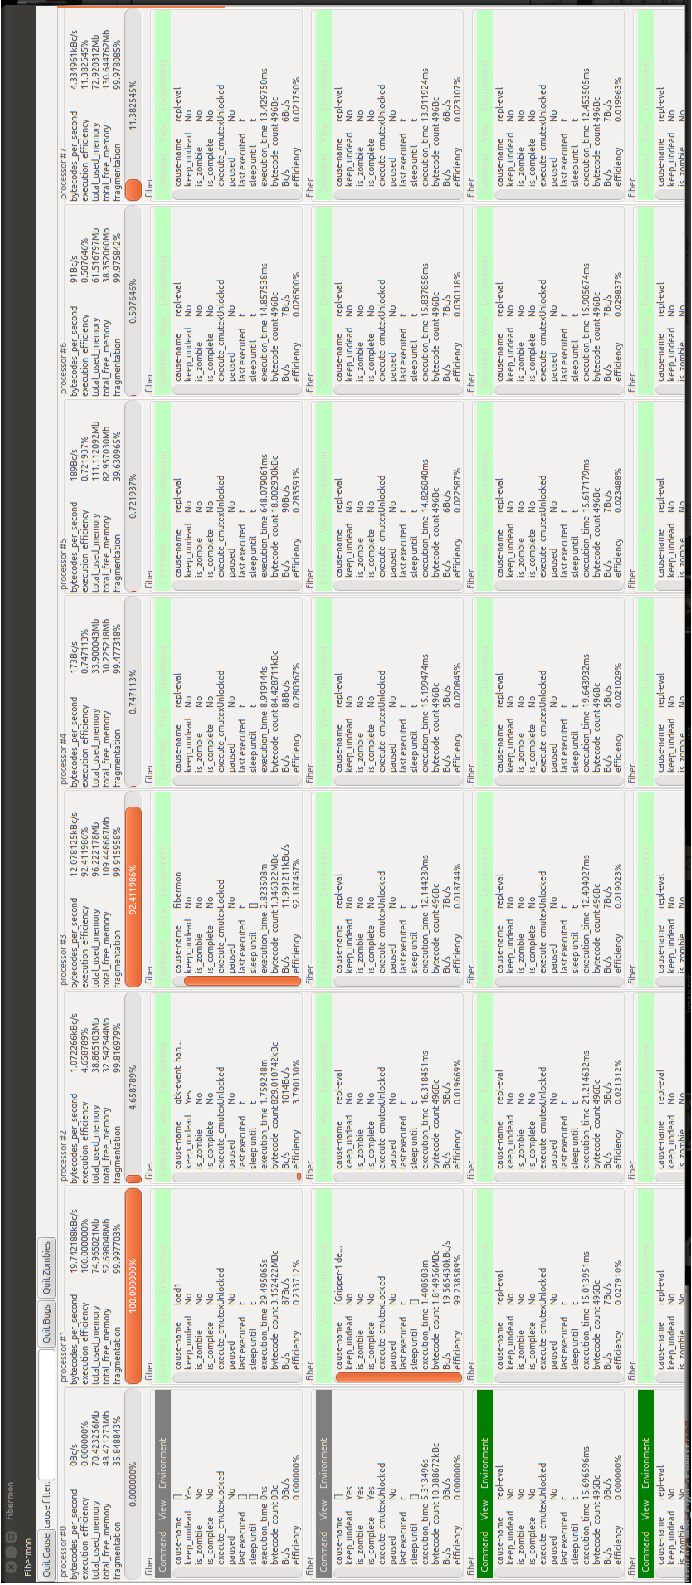
\includegraphics[width=10cm]{gfx/fibermon_many_fibers}
  \caption[FiberMon application monitoring many fibers]{FiberMon
    application monitoring hundreds of parallel fibers, simulated
    activities in Duration, executing on eight different physical
    processor cores.}
  \label{figure:fibermon_many_fibers}
\end{figure}

\section{Pausing and Resuming Activities}

SALS includes a {\tt pause} command to pause the current fiber:
\begin{equation*}
\text{\tt [pause]}
\end{equation*}
The {\tt pause} command causes the executing fiber to remove itself
from the scheduler, after removing itself, it yields the rest of the
scheduler cycle.  A fiber that is paused in this sense uses none of
SALS's processor resources because it is completely removed from
the scheduler.

If a fiber has paused, it cannot restart itself.  In order for a fiber
to resume execution, another executing fiber must use the
{\tt resume} command with the fiber object as an argument:
\begin{equation*}
\text{\tt [resume <fiber>]}
\end{equation*}

The {\tt pause} and {\tt resume} commands are extremely efficient for
managing large simulations in which most fibers will be inactive at
any given time, but they are a little cumbersome, so I have written a
lightweight and helpful \emph{fiber trigger} object, which I will
explain after explaining one more object that is used to program fiber
triggers.

\section{Mutual Exclusion}

SALS provides a primitive object called a \emph{mutex} for handling
the mutually exclusive access to resources.  A mutex object has two
possible states: locked and unlocked.  If the mutex object is unlocked
then when a fiber tries to locks the mutex, the mutex switches to the
locked state and the fiber continues execution.  If the mutex object
is already locked when a fiber tries to lock the mutex, the fiber will
pause until the mutex is unlocked, at which point the mutex will be
locked and the waiting fiber will resume execution.  Mutexes are used
for protecting shared resources from being used by more than one fiber
at a time.

Mutexes are a special type of object that must be supported by the
hardware of a concurrent computer.  Almost every parallel programming
language has a mutex construct that derives from this hardware mutex.
So, mutexes are common to parallel programming, but they are
notoriously difficult to debug, resulting in bugs affectionately
referred to as ``race conditions'' or ``deadlocks''.  In order to help
with debugging these types of problems, mutexes in SALS keep track of
which fibers are waiting for the lock or holding the lock.  I have
found this extra information invaluable in debugging complicated mutex
related bugs.

\section{Fiber Triggers}

The fiber trigger organizes sets of paused fibers so that they can be
woken up at the same time.  Basically, the fiber trigger is an object
that provides a useful abstraction for controlling fiber execution
that combines a mutex with the {\tt pause} and {\tt resume} commands.

A fiber can be added to the resume set of a fiber trigger by using the
{\tt wait-for-trigger} command as in the following example:
\begin{equation*}
\text{\tt [wait-for-trigger <fiber-trigger>]}
\end{equation*}
The {\tt wait-for-trigger} command atomically pauses the current fiber
and then adds the fiber to resume queue of the fiber trigger object.  The fiber trigger object provides a mutex object 

\section{leftovers...}

\section{Fiber Complete and Bug Found Triggers}

get fiber triggers from fiber objects.

execution complete versus bug found.


\section{{\tt par-fib}}

\begin{equation*}
\begin{array}{l}
\text{\tt [defunk par-fib [n]} \\
\text{\tt ~~[if [== n 0]} \\
\text{\tt ~~~~~~0} \\
\text{\tt ~~~~[if [== n 1]} \\
\text{\tt ~~~~~~~~1} \\
\text{\tt ~~~~~~[let [[x []]} \\
\text{\tt ~~~~~~~~~~~~[y []]]} \\
\text{\tt ~~~~~~~~[parog [= x [par-fib [- n 2]]]} \\
\text{\tt ~~~~~~~~~~~~~~~[= y [par-fib [- n 1]]]]} \\
\text{\tt ~~~~~~~~[+ x y]]]]]}
\end{array}
\end{equation*}


\section{Symbolic Statements in SALS}

\section{Three Categories of Symbol}

SALS programming expressions are combinations of symbols in lists.
It is important to keep all of these symbols straight.  I have so far
introduced three slightly different conceptions of symbols: (1) the
symbols that are reflectively symbolized from the activities of
Duration, (2) the symbols that a programmer types into a computer, and
(3) the simulated symbols that are generated by the simulated
first-order reflective layer of thinking.

\section{Concurrent Memory Allocation Pools}

SALS works off of a multiple pool memory allocation system that
allows separate pools for each concurrent virtual processor,
eliminating the need for many lock situations that occur with shared
memory pools.

\section{Garbage Collection}



\section{Layered Cognitive Architecture}

On this computational substrate, I have built a layered cognitive
architecture that is inspired by Minsky's description of the bottom
four layers of his Emotion Machine, or Model-6 architecture.  This
includes, a physical world, a reactive mapping of the physical world
to pre-symbolic activities, a first-order reflective thinking layer
that creates symbols, causal models, and plans for accomplishing
physical goals, as well as a second-order reflective thinking layer
that creates symbols, causal models, and plans for accomplishing
first-order thinking goals.  The model behind this implementation
inductively explains how this implementation can be extended to an
arbitrary number of reflective thinking layers.  While this part of
the thesis is primarily focused on the simulation of a static,
modelled representation of this model, I derive the fundamental basis
of my model of mind in non-technical English in
\autoref{part:the_model}.

\section{Block Building Domain}

My architecture exists in three main parts: the physical layer, the
first-order reflective layer, and the second-order reflective layer.
In order to explain how my model allows for learning at multiple
levels, I use a simulation of a physical domain that is easy to
understand.  I use this simulation primarily for communication of my
working model by demonstrating learning at multiple reflective levels
in response to a single physical failure.

My simulation of the physical block building domain is meant to appear
as similar to the canonical toy problem, \emph{Blocks World}, with one
key exception: my model is meant to have a different interpretation
than the original Blocks World.  The primary point to emphasize here
is that my physical simulation is meant to represent a dynamic
physical world as opposed to the logical and completely static
reference for the Blocks World physical domain.



\section{Reactive Layer}

The physical layer in my model is implemented by combining the
physical simulation with a reactive layer that maps the physical
simulator perceptual and motor functions to ``sub-symbolic''
activities that are available to first-order reflection.




%*****************************************
\chapter{Related Implementations}
\label{chapter:related_implementations}
%*****************************************


%%************************************************
\chapter{Learning to Accomplish Goals}\label{ch:learning_to_accomplish_goals}
%************************************************

\begin{quote}
  Problem-solvers must find relevant data.  How does the human mind
  retrieve what it needs from among so many millions of knowledge items?
  Different AI systems have attempted to use a variety of different
  methods for this.  Some assign keywords, attributes, or descriptors to
  each item and then locate data by feature-matching or by using more
  sophisticated associative data-base methods.  Others use
  graph-matching or analogical case-based adaptation.  Yet others try to
  find relevant information by threading their ways through systematic,
  usually hierarchical classifications of knowledge---sometimes called
  ``ontologies''.  But, to me, all such ideas seem deficient because it
  is not enough to classify items of information simply in terms of the
  features or structures of those items themselves.  This is because we
  rarely use a representation in an intentional vacuum, but we always
  have goals---and two objects may seem similar for one purpose but
  different for another purpose.
\end{quote}
\begin{flushright}
  --- \defcitealias{minsky:1991}{Marvin Minsky}\citetalias{minsky:1991}
\end{flushright}

% horvat: -^^^
%
%  very true
%  you could disuss it in paralell to the view that “mind
%  is a system always evolving” (Hoya, 2005)
%

In this introductory chapter I will give an overview of the problem of
reflectively learning to accomplish goals.  First, I will develop the
assumption that any process that I choose under given constraints can
be reflectively monitored and useful information, e.g. beginning and
ending times, will be temporarily stored.  In other words, I assume
that my system natively supports procedural reflection for all
processes.  Given this assumption, I show in this chapter that the
problem of building a system that learns to accomplish goals in its
environment becomes a simple loop-less causal structure involving at
least four different types of learning.  These four types of learning
complete a circle of causal learning from goals through actions to
physical states and back to goals, but because of time, causality is
still in an ordered lattice structure beginning with goals as the
causal roots for all other knowledge.

In later chapters I will introduce experiments I have performed in
different physical problem simulations.  The first is a simple
proof-of-concept demonstration of my reflective learning algorithm in
a blocks world problem domain.  Also, I show my reflective
architecture extended to a larger physical reasoning domain, including
multiple agents learning to cook together in a kitchen environment.
In this larger problem space, agents can communicate high-level
procedures specified in a simple programming language that is shared
by the agents, and refers to both mental and physical actions of the
agents.

\section{The Agent-Environment Model}

\begin{figure}[bth]
  \center
  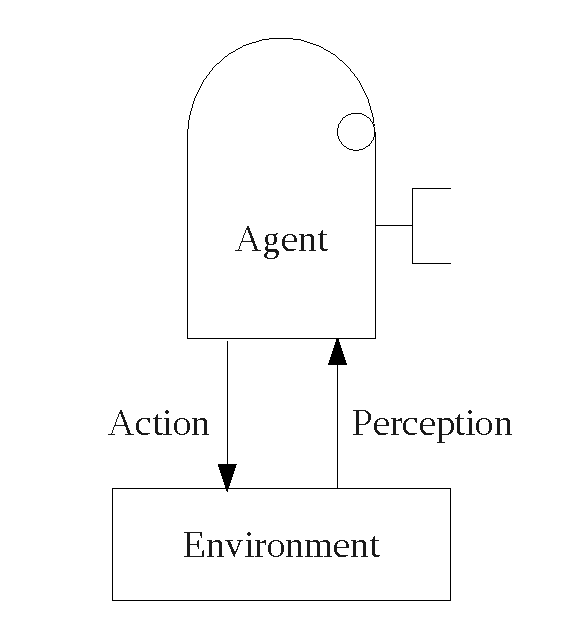
\includegraphics[height=5cm]{gfx/agent_environment}
  \caption[The agent-environment model]{The agent-environment model.}
  \label{fig:agent_environment}
\end{figure}

Figure~\ref{fig:agent_environment} shows the basic agent-environment
model.  In this model, I make a distinction between the environment
and the agent.  At any given time, the agent and the environment are
each represented as a specific static form of data.  Further, these
representations change over time, according to a given transfer
function.  I will treat this system as a deterministic system,
although one could imagine adding random variables to the transfer
function: the basic theory is the same.  It is easier to add
randomness to a deterministic theory than the opposite.  There are
also many benefits to developing a deterministic model with perhaps a
pseudorandom aspect because this allows for the repeatability of
scientific experiments, for which the model may be used as a metric.
The two processes communicate information along two channels: (1) an
action channel from the agent to the environment, and (2) a perception
channel from the environment to the agent.


\section{The State-Action Model}
\label{sec:state_action_model}

\begin{figure}[bth]
  \center
  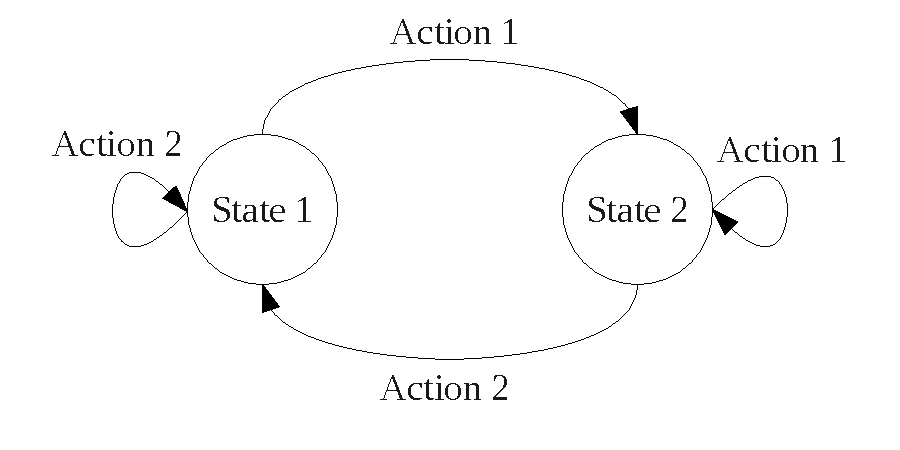
\includegraphics[width=6cm]{gfx/state_action}
  \caption[The state-action model]{The state action model.  Two states
    are represented by nodes and two actions are represented by edges
    from each of the two states.}
  \label{fig:state_action}
\end{figure}

The agent is in an environment, which is in a specific state.  My
agent performs an action, which can affect the state of the
environment.  Figure~\ref{fig:state_action} shows a simple \ac{FSM}
state-action model, which has two states for the environment and two
actions for the agent to perform in each of these states.  The
state-action model is a simple model for how actions map to changes in
the state of the environment.


\section{A Multiple Agent-Environment Model}

\begin{figure}[bth]
  \center
  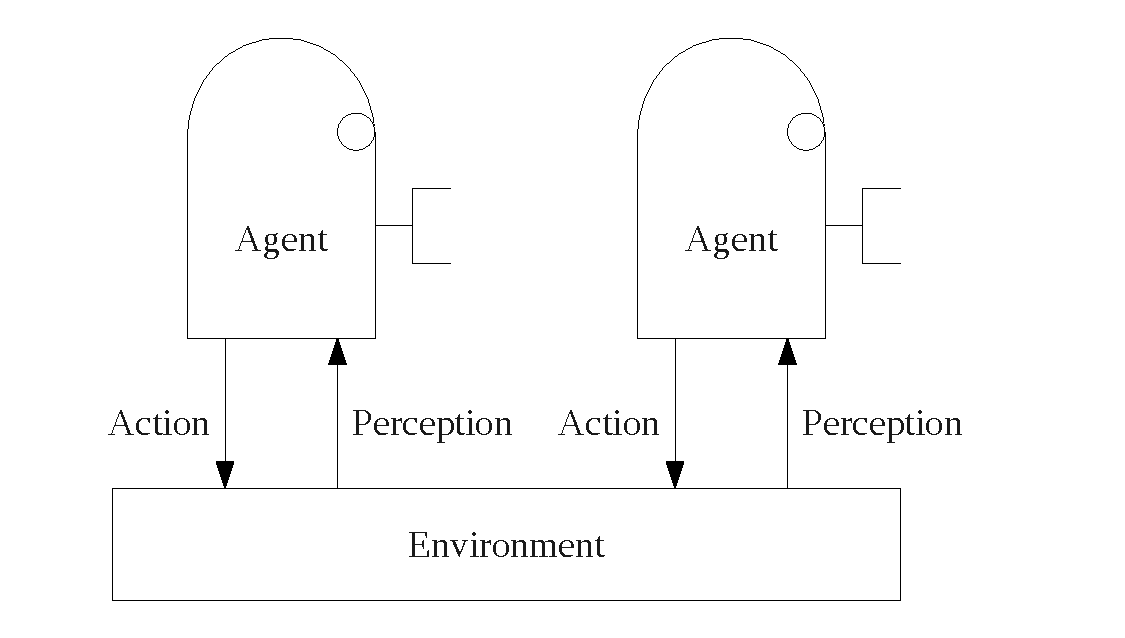
\includegraphics[height=5cm]{gfx/multiple_agent_environment}
  \caption[The multiple agent environment model]{The multiple agent environment model.}
  \label{fig:multiple_agent_environment}
\end{figure}

In order to model social intelligence, we introduce the multiple agent
environment model shown in
Figure~\ref{fig:multiple_agent_environment}.


\section{Agent Process Communication}

Because agent processes can only directly act on and perceive the
environment, all communication between agent processes must occur
through the environment process.  We assume that agents can
communicate some form of symbolic knowledge structure in the absence
of noise.  These representations are used to communicate processes
from one agent to another.  Specific examples of such a process
representation that we have used in our experiments are described in
more detail in
Sections~\ref{sec:serial_process_representation}--\ref{sec:parallel_process_representation}.


\section{A Relational State Representation}

\begin{figure}[bth]
  \center
  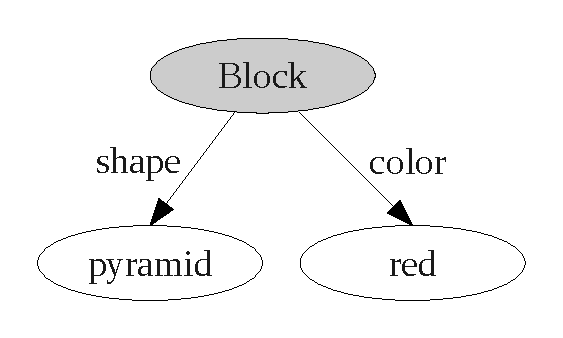
\includegraphics[height=3cm]{gfx/frame_representation}
  \caption[Frame-based relational representation]{Frame-based relational representation.}
  \label{fig:frame_representation}
\end{figure}

See Figure~\ref{fig:frame_representation}.

\section{Introducing Reflection Early in the Process}

Now, I have introduced my problem as being divided into at least two
processes, at least one agent process and an environment process.
Further, I have introduced how a basic process may be thought of as an
\ac{FSM}.  At this point, I introduce a model for keeping track of the
changes in a computational process: reflective knowledge.  I
purposefully make this assumption before I define the details of the
agent model process because, in my approach, I would like to
reflectively reason about potentially any aspect of this agent
process.

\section{Reflective Knowledge}

\begin{figure}[bth]
  \center
  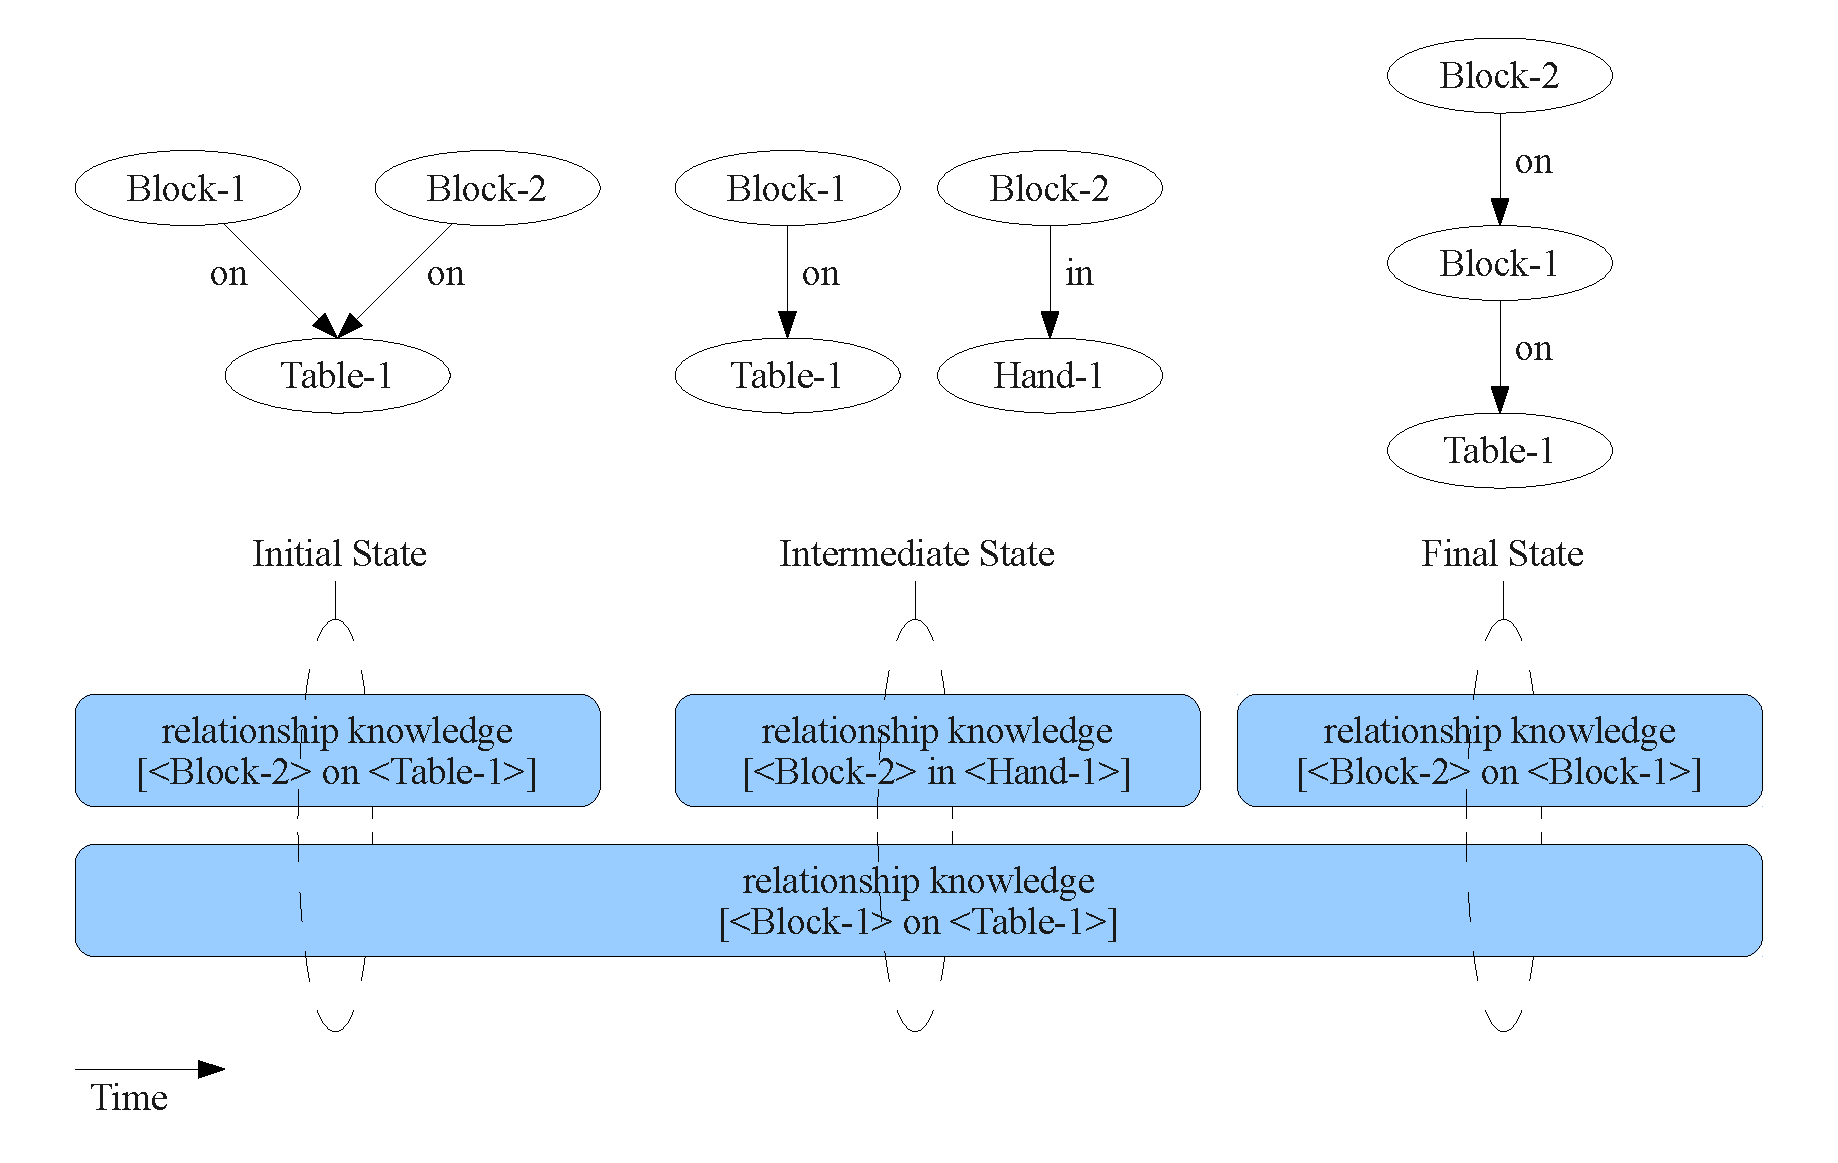
\includegraphics[width=12cm]{gfx/reflective_event_representation}
  \caption[A reflective event representation]{A reflective event representation shows the changes in a labeled graph.}
  \label{fig:reflective_event_representation}
\end{figure}


While the term meta-knowledge is used to describe the very general
idea of knowledge about knowledge, I use the term reflective knowledge
to refer to the specific type of meta-knowledge that refers to
knowledge about the changes to a knowledge structure.  If I keep track
of the changes to a knowledge structure, I can later integrate these
changes in order to obtain an equivalent form of that knowledge
structure as it was at any point in the past.\footnote{See
  Section~\ref{sec:what_is_a_computer} for a discussion of more
  realistic models of computation, including multiple-core and cluster
  models.}




\section{Frame Perceptions}

\begin{figure}[bth]
  \center
  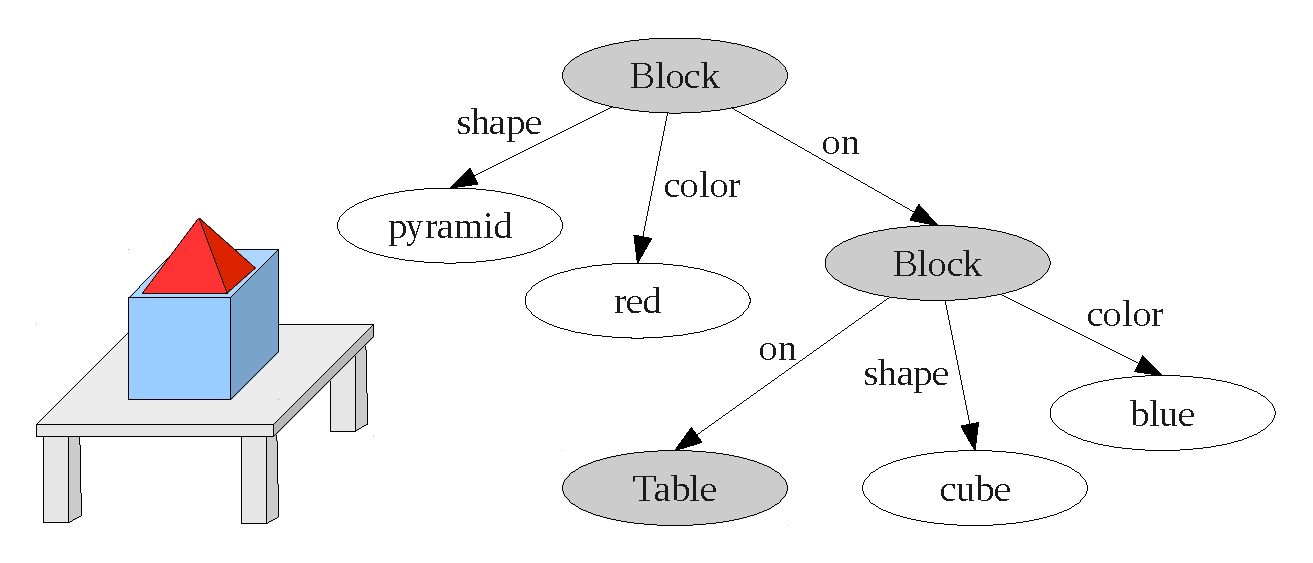
\includegraphics[height=5cm]{gfx/frame_perception}
  \caption[Collections of frames used as perceptual input to agent]{Collections of frames used as perceptual input to agent.}
  \label{fig:frame_perception}
\end{figure}

See Figure~\ref{fig:frame_perception}.


\section{Partially Observable State Model}

\begin{figure}[bth]
  \center
  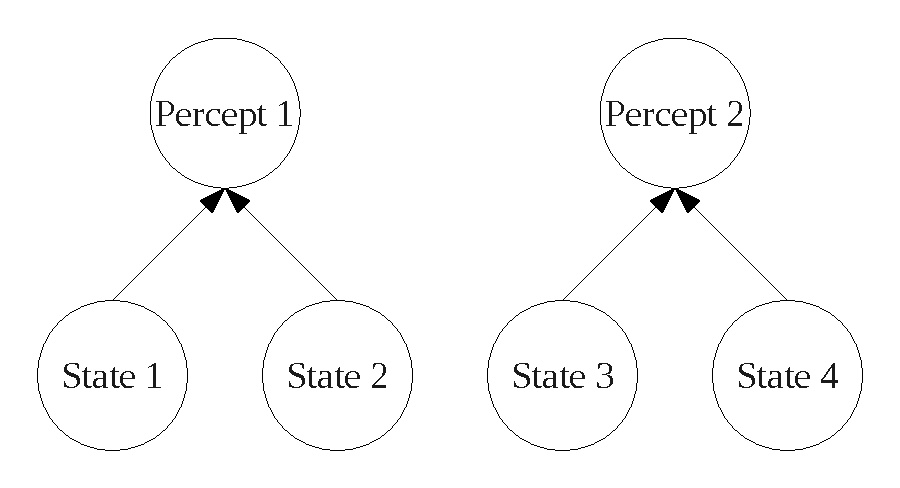
\includegraphics[width=6cm]{gfx/partially_observable}
  \caption[The partially observable state model]{The partially observable model.}
  \label{fig:partially_observable}
\end{figure}

\begin{figure}[bth]
  \center
  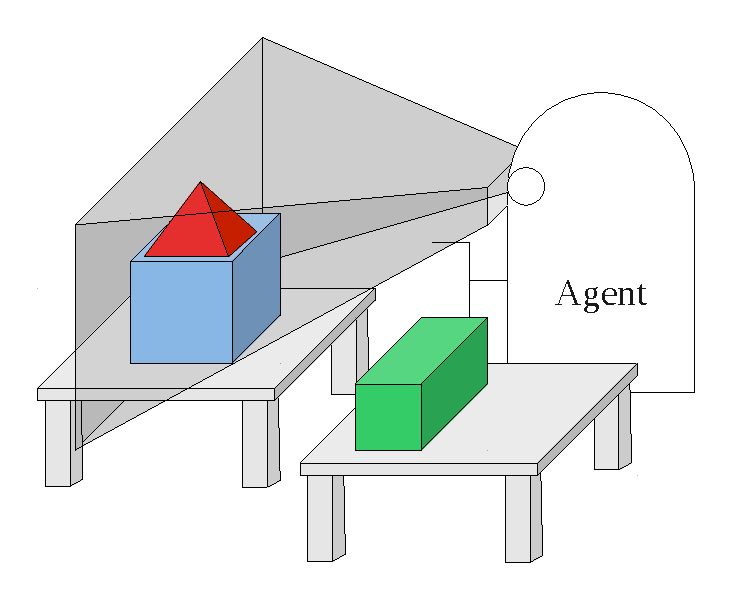
\includegraphics[height=5cm]{gfx/partial_frame_perception}
  \caption[The state of the environment is only partially
    observable]{The state of the environment is only partially
    observable.}
  \label{fig:partial_frame_perception}
\end{figure}

The agent process does not have complete access to the state of its
environment.  The agent's perceptual stream of information depends on
the state of the environment, but it is a function of the environment
and not the actual state of the environment.  In other words, the
perceptual state that is communicated from the environment to the
agent is an injective function mapping the environment to the
perception of the agent.  See
Figures~\ref{fig:partially_observable}~and~\ref{fig:partial_frame_perception}
for two examples of partially observable environments.


\section{Agent Abstract Physical Model}

\begin{figure}[bth]
  \center
  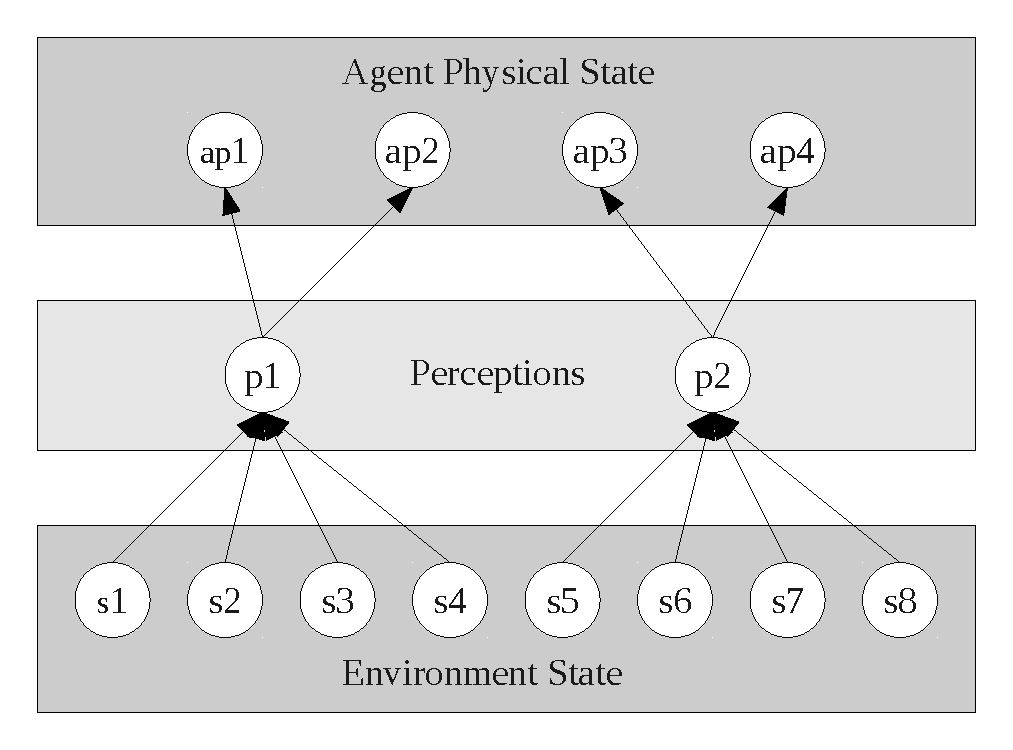
\includegraphics[width=8cm]{gfx/environment_perception_physical}
  \caption[The agent has an abstract physical model of the
    environment]{The agent has an abstract physical model of the
    environment.}
  \label{fig:environment_perception_physical}
\end{figure}

See Figure~\ref{fig:environment_perception_physical}.


\section{A Physical Goal Representation}

\begin{figure}[bth]
  \center
  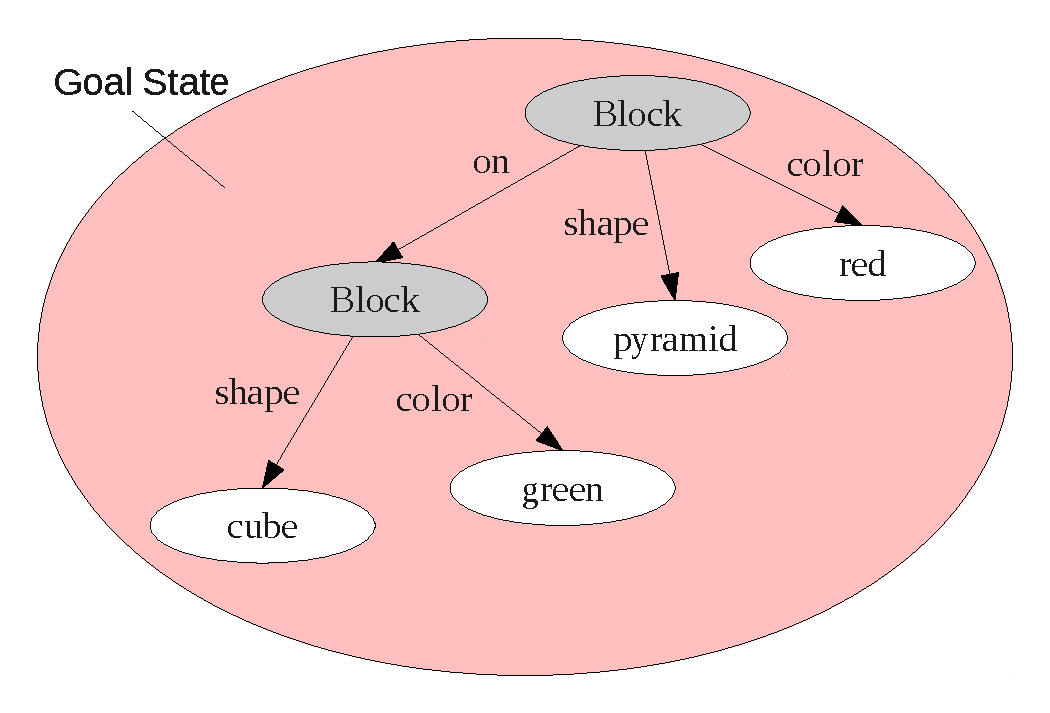
\includegraphics[height=4cm]{gfx/goal_state}
  \caption[A physical goal representation]{A physical goal
    representation is a structural relationship that may or may not
    currently exist within the physical knowledge base.}
  \label{fig:goal_state}
\end{figure}

See Figure~\ref{fig:goal_state}.


\section{The Reflective Learning Cycle}

\begin{figure}[bth]
  \center
  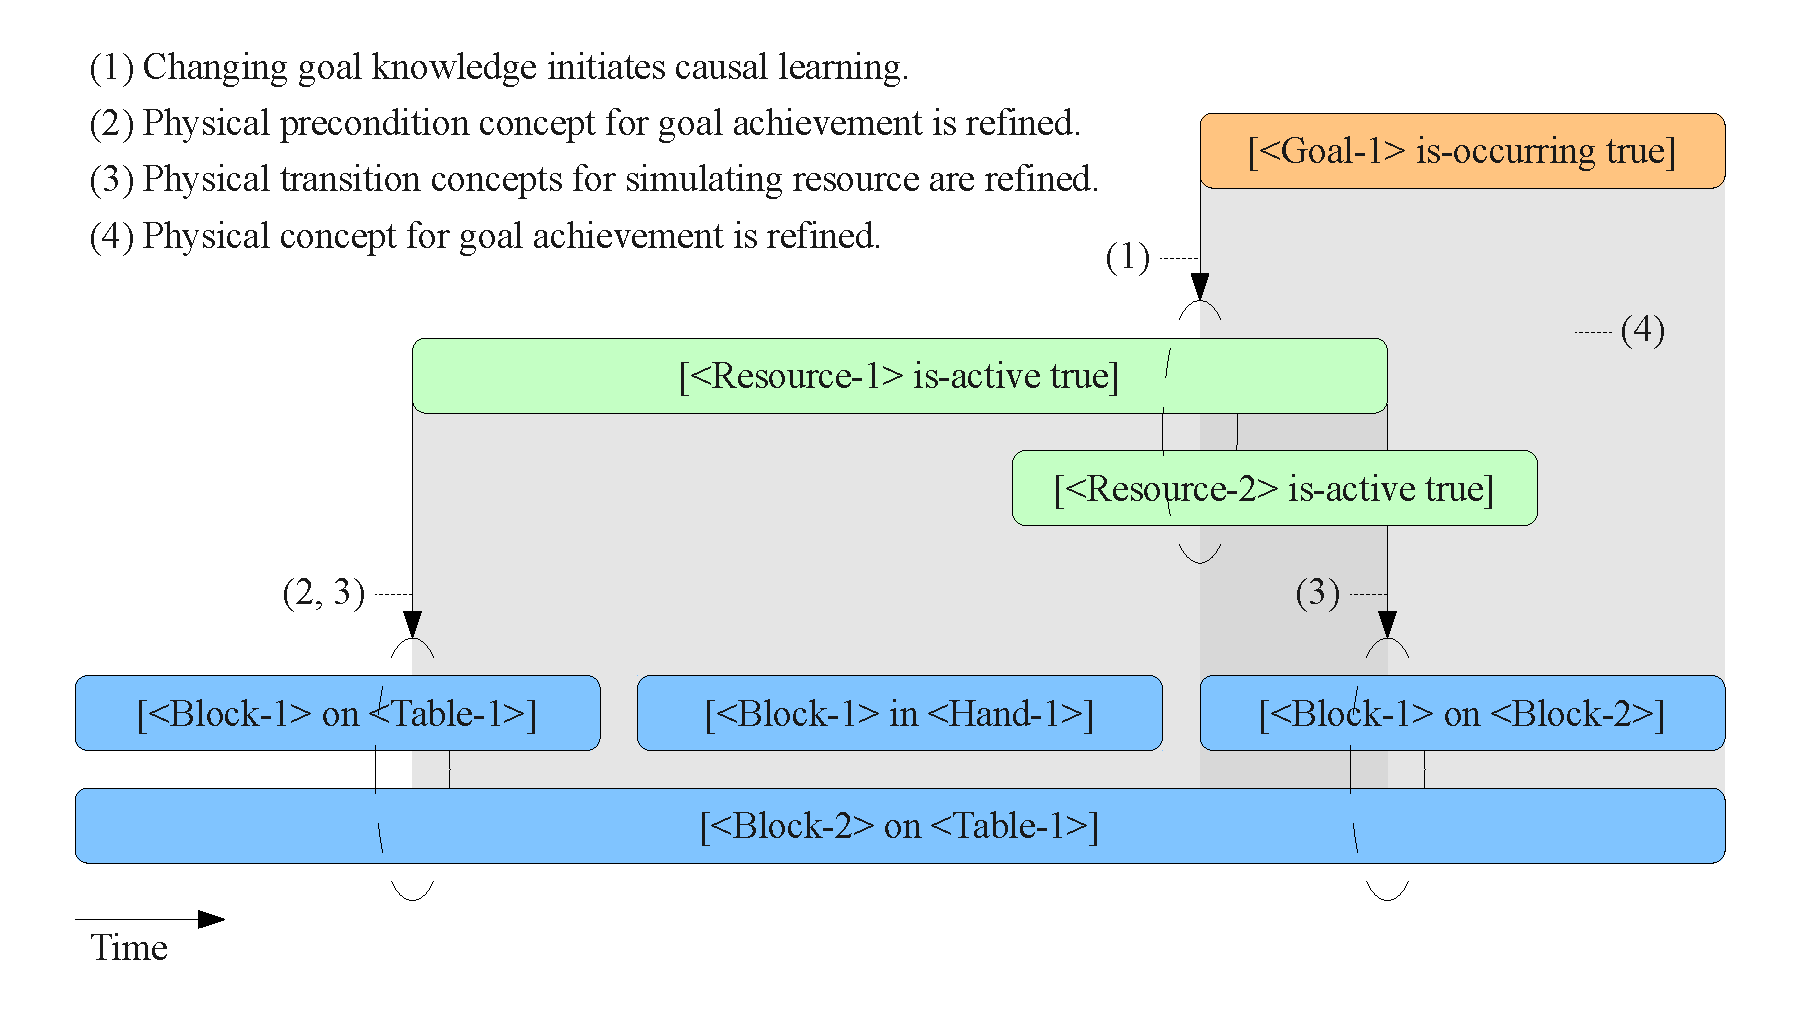
\includegraphics[width=12cm]{gfx/learning_to_plan}
  \caption[The reflective learning cycle]{The reflective learning
    cycle is a way to learn knowledge used to plan toward goals that
    maintains the causal dependency structure of the knowledge.}
  \label{fig:learning_to_plan}
\end{figure}

A system without a goal has no reason to learn the effects of its
actions.  Figure~\ref{fig:learning_to_plan} shows how the process of
learning causal models relating reflective states to physical states
is a fundamentally goal-driven process.  We show how this goal
prediction process leads to at least a four step causal chain of
knowledge learning.  It is important to point out that although the
learning process is a cycle over time, this ends up creating a causal
structure for knowledge dependency without loops---a critical property
in general to maintain for any causal representation.

These four goal-oriented cyclical learning steps build four of the
major types of knowledge that my goal-oriented inference and planning
system uses.  Let us now briefly introduce these four types of
knowledge before going into a more thorough explanation of the utility
of each.

\begin{enumerate}

\item{Goal-oriented action hypotheses: focuses and constrains the
  initial action learning search.}

\item{Action physical precondition goal occurrence hypotheses: allows
  predicting whether or not an action will accomplish the given goal
  under a given physical precondition.}

\item{Action physical precondition trans-frame hypotheses: allows for
  physically simulating the given action in a given physical state.}

\item{Physical hypotheses for predicting goal occurrence: allows for
  predicting if a given physical state implies that the goal is
  occurring.}

\end{enumerate}

Note that there are two different concepts of time that are displayed
in Figure~\ref{fig:learning_to_plan}.  It is important to not confuse
these.  The first kind of time is represented by the sequence of
change events in the knowledge structure that was reflectively traced
in order to generate the temporal event representation shown in the
figure.  This first time is represented and labelled as the horizontal
axis in the figure.  The second kind of time represented in the figure
is represented by the enumeration of the four learning steps.  This
learning process is a reflective learning process because it learns
from reflective knowledge gathered from tracing processes.

In the following four sections, we will describe the utility of each
of these four different types of learned knowledge in more detail.

\section{Goal-Oriented Action Hypotheses}
\label{sec:goal_oriented_action_hypotheses}

\begin{figure}[bth]
  \center
  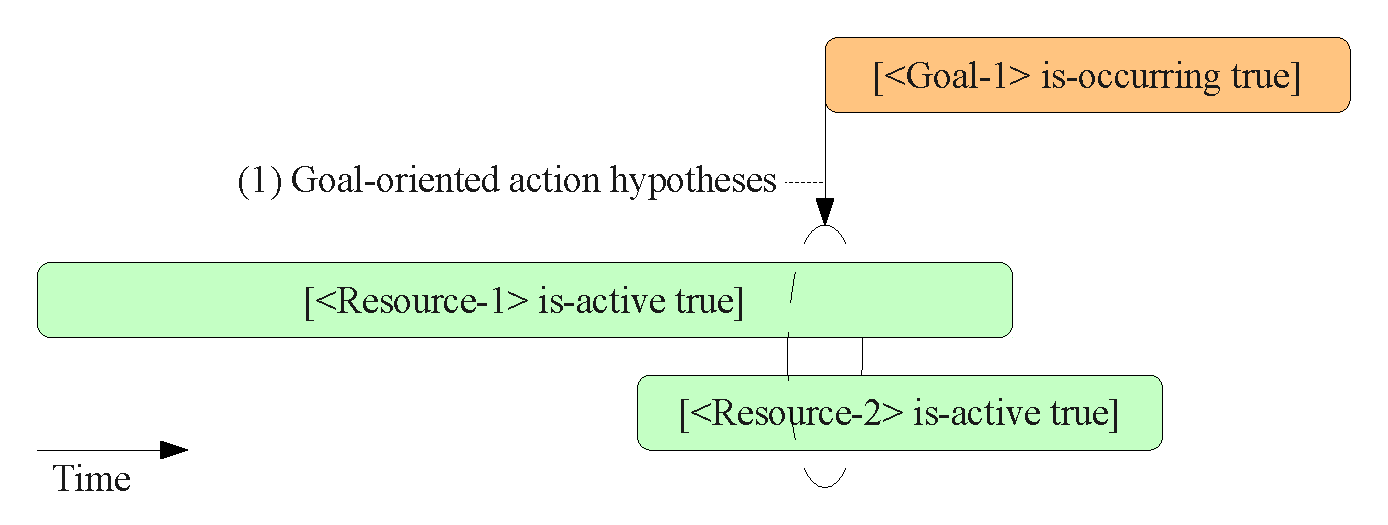
\includegraphics[width=11cm]{gfx/learning_to_plan-1-goal_oriented_action_hypotheses}
  \caption[Goal-oriented action hypothesis knowledge]{Goal-oriented action hypothesis knowledge.}
  \label{fig:goal_oriented_action_hypotheses}
\end{figure}

Figure~\ref{fig:goal_oriented_action_hypotheses} shows the first step
of the reflective learning cycle.  This first step of the learning
cycle is caused reflectively by the goal event beginning to exist.
When a goal event comes into existence, a reflective process
monitoring this goal knowledge makes a list of potential actions that
might be useful for causally predicting this goal condition in the
future.  In the figure we can see that a simple interval-point
intersection operation between the beginning point of the goal event
and any action event interval is enough to generate two actions as
initial causal hypotheses.  See
Section~\ref{sec:goal_oriented_action_hypotheses_generation_techniques}
for details on the techniques that I used for generating goal-oriented
action hypotheses in my system.


\section{Action Precondition Goal Occurrence Hypotheses}

\begin{figure}[bth]
  \center
  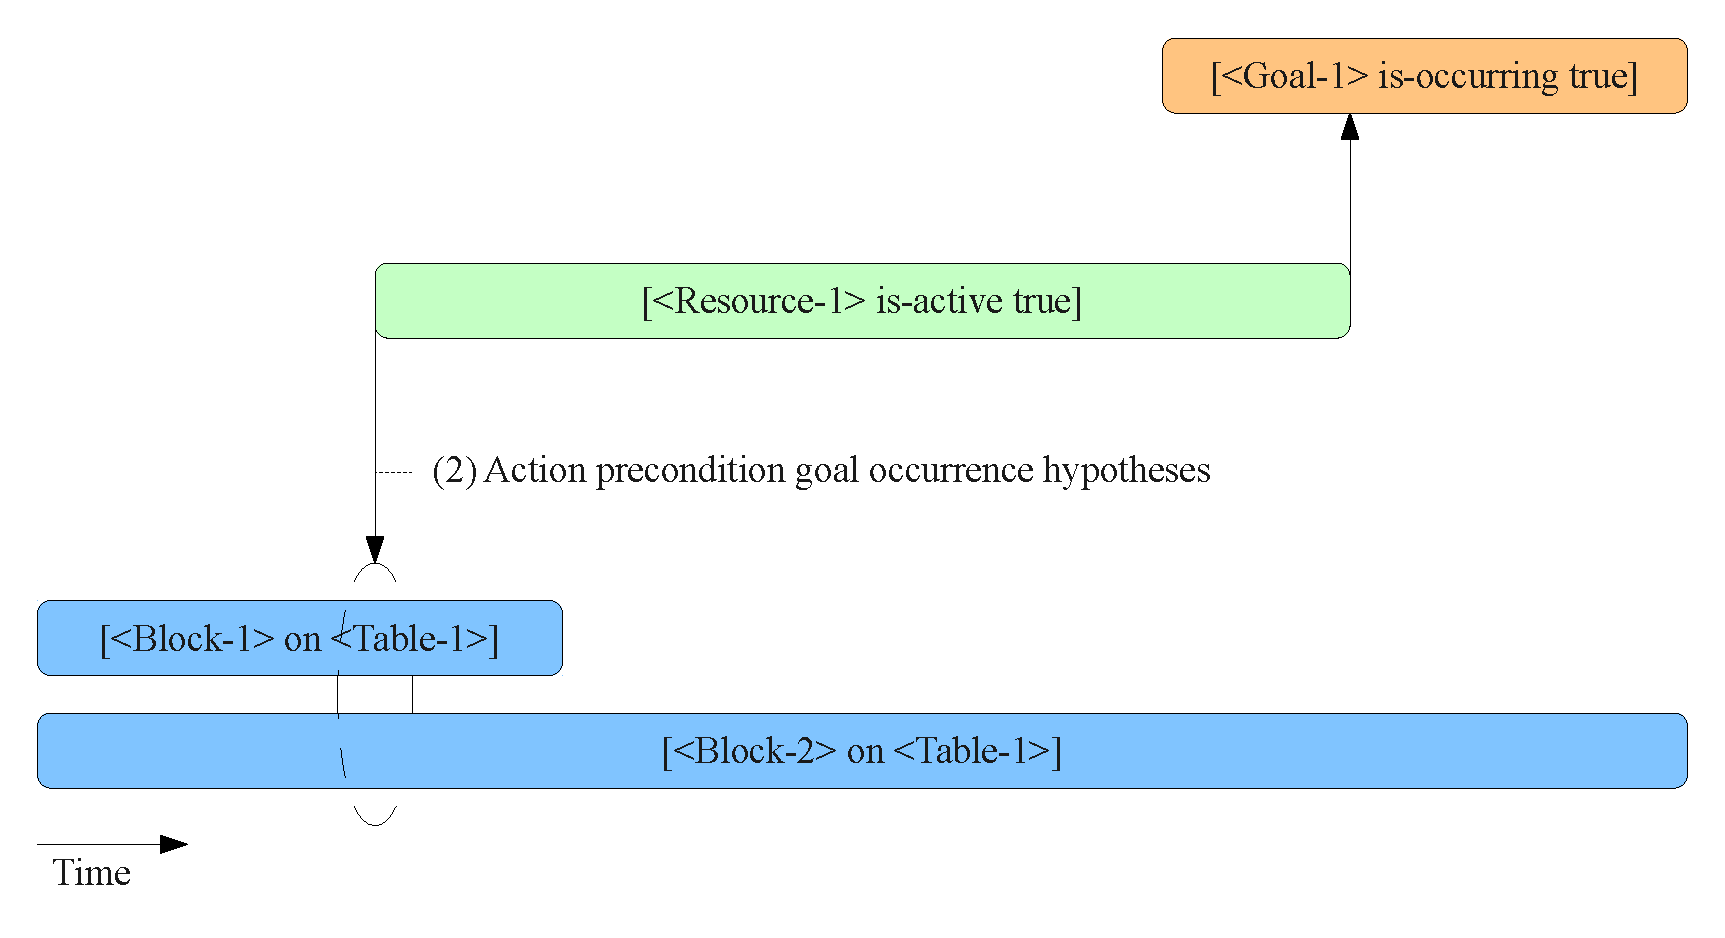
\includegraphics[width=11cm]{gfx/learning_to_plan-2-action_precondition_goal_occurrence_hypotheses}
  \caption[Action precondition goal occurrence hypotheses]{Action precondition goal occurrence hypotheses.}
  \label{fig:action_precondition_goal_occurrence_hypotheses}
\end{figure}

See Figure~\ref{fig:action_precondition_goal_occurrence_hypotheses}.


\section{Action Precondition Trans-Frame Hypotheses}

\begin{figure}[bth]
  \center
  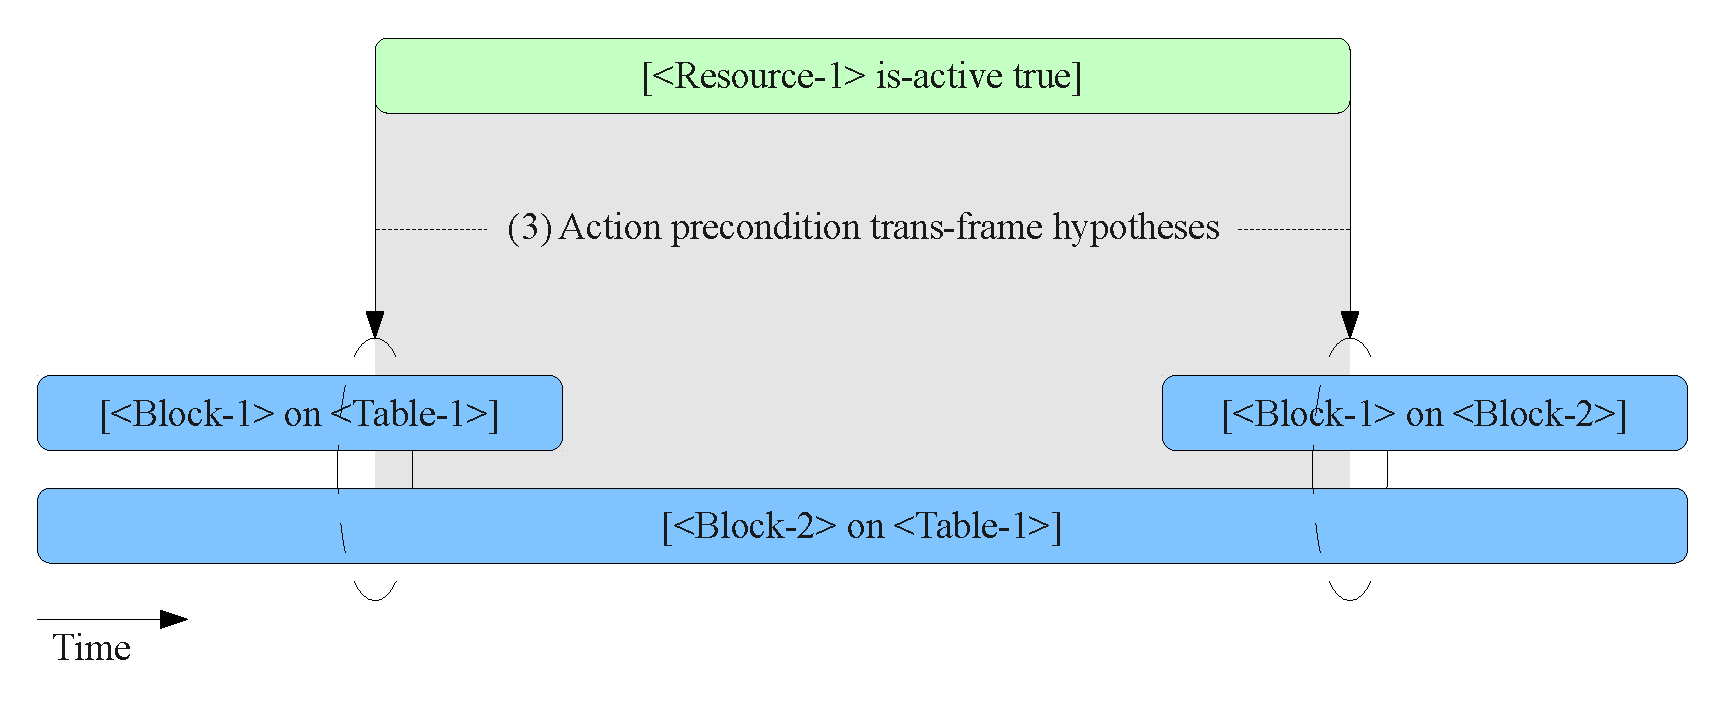
\includegraphics[width=11cm]{gfx/learning_to_plan-3-action_precondition_transframe_hypotheses}
  \caption[Action precondition trans-frame hypotheses]{Action precondition trans-frame hypotheses.}
  \label{fig:action_precondition_transframe_hypotheses}
\end{figure}

See Figure~\ref{fig:action_precondition_transframe_hypotheses}.


\section{Physical Hypotheses for Predicting Goal Occurrence}

\begin{figure}[bth]
  \center
  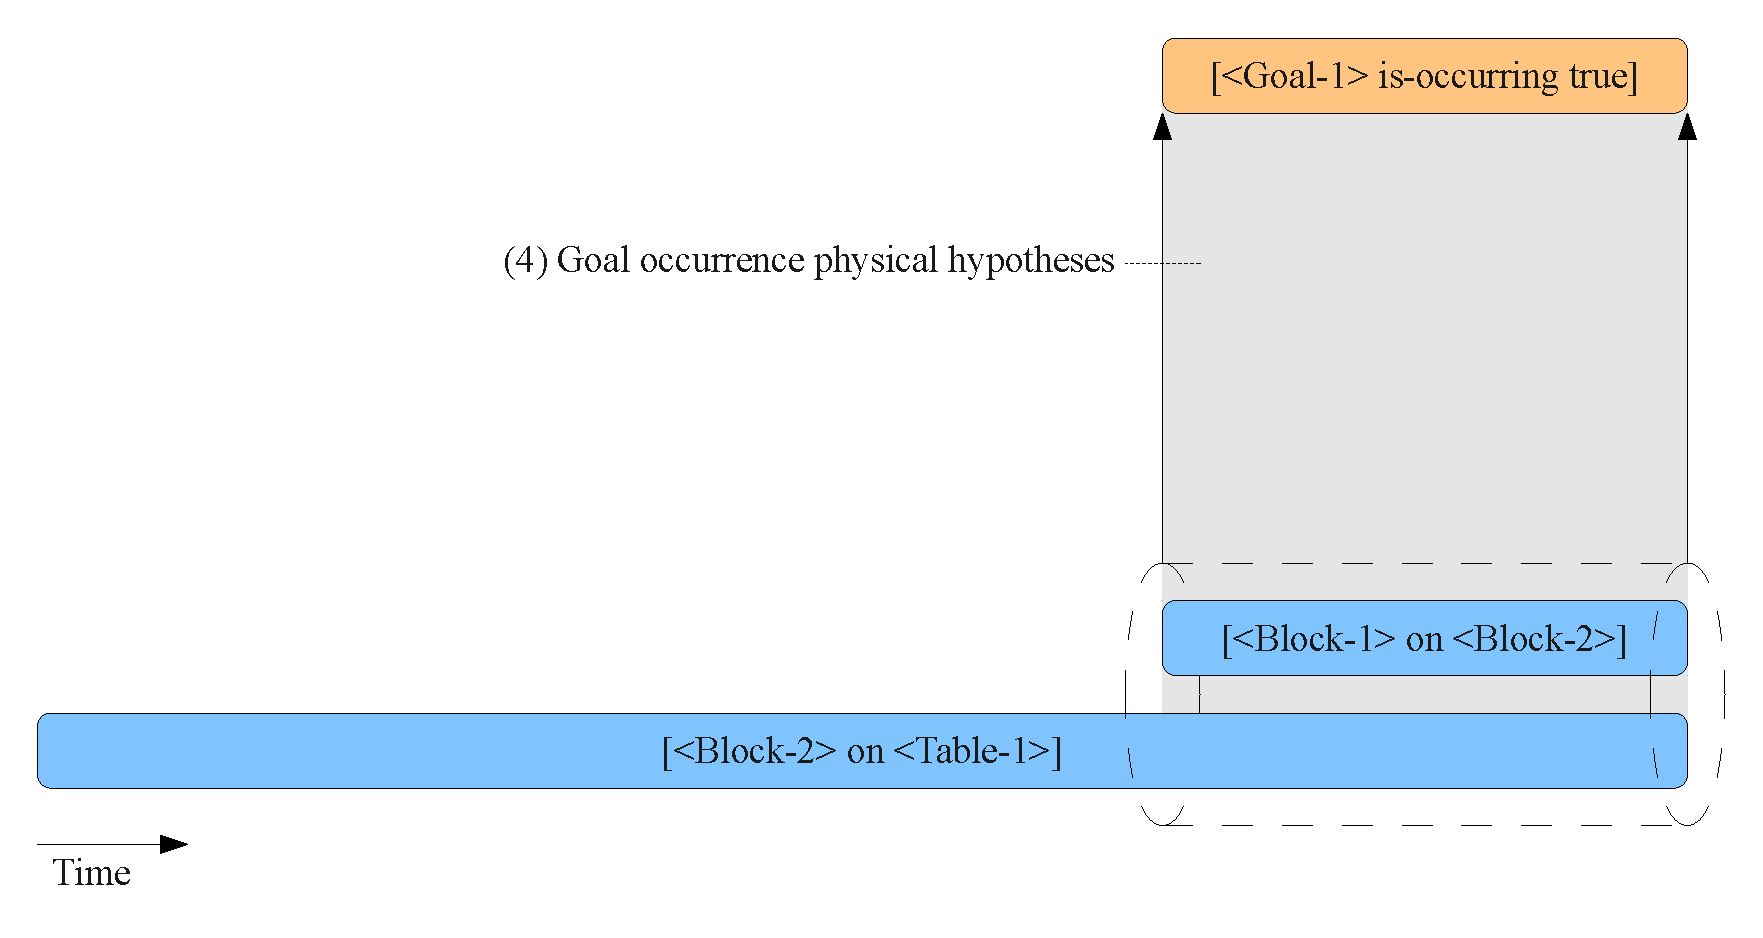
\includegraphics[width=11cm]{gfx/learning_to_plan-4-goal_occurrence_physical_hypotheses}
  \caption[Goal occurrence physical hypotheses]{Goal occurrence physical hypotheses.}
  \label{fig:goal_occurrence_physical_hypotheses}
\end{figure}

See Figure~\ref{fig:goal_occurrence_physical_hypotheses}.


\marginpar{\emph{learning goal}: focusing learning on a subset of the state space.}


\section{Learning Trans-Frames for Events}
\label{sec:learning_trans_frames_for_events}

\begin{figure}[bth]
  \center
  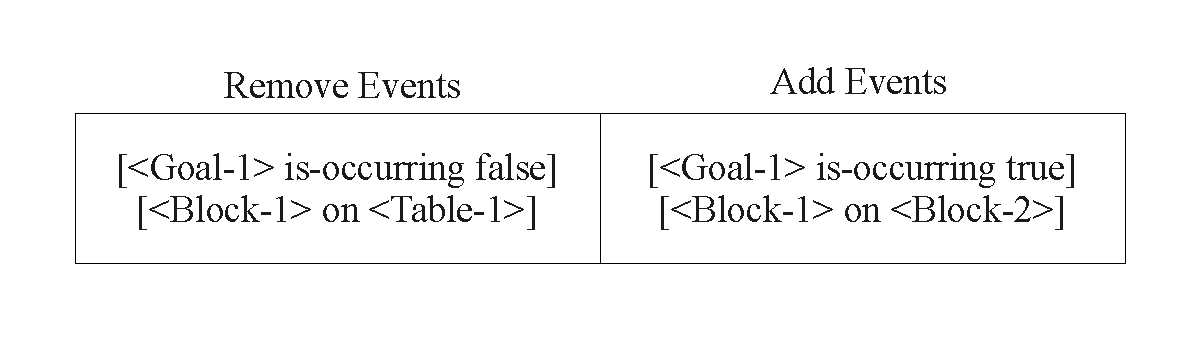
\includegraphics[width=10cm]{gfx/transframe}
  \caption[A trans-frame for an event]{A trans-frame for an event is a
    list of differences in knowledge between the beginning and ending
    of the event.}
  \label{fig:transframe}
\end{figure}

See Figure~\ref{fig:transframe}.  Also, trans-frames of trans-frames
can be thought of as a form of analogical transfer, which I further
discuss in
Section~\ref{sec:learning_analogies_as_differences_of_differences}.


\section{Partially-Ordered Plan Representation}

\begin{figure}[bth]
  \center
  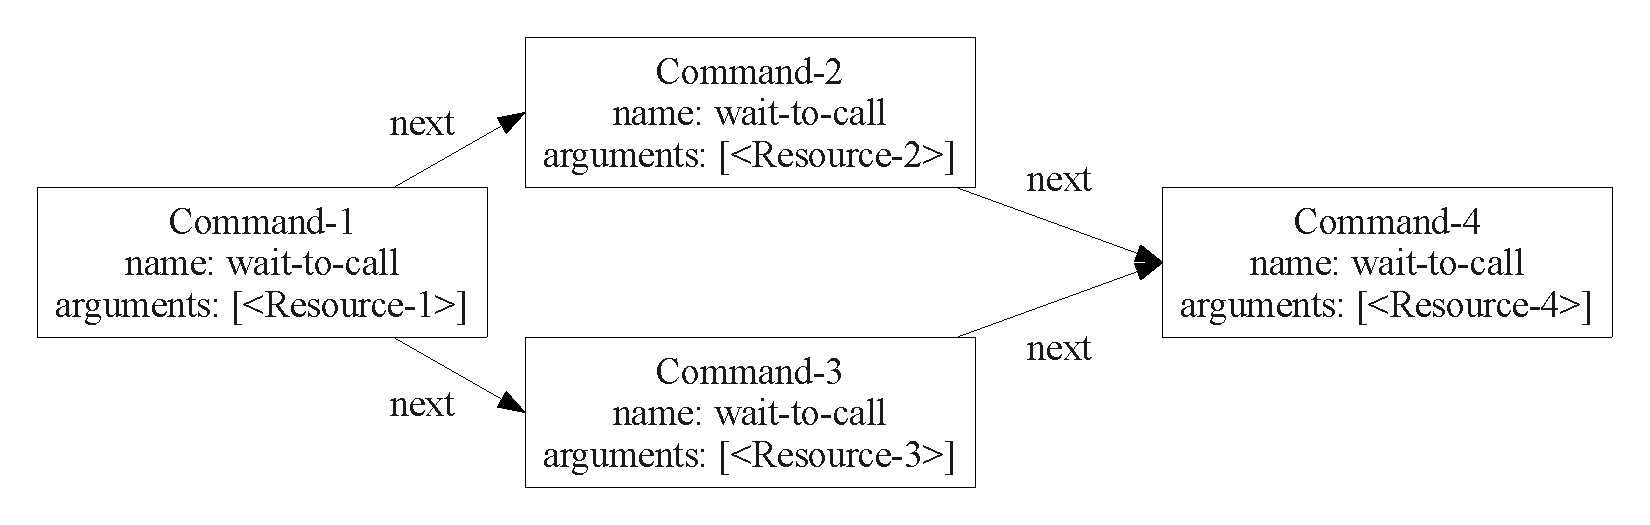
\includegraphics[width=11cm]{gfx/serial_and_parallel_plan}
  \caption[A partially-ordered plan with serial and parallel
    components]{A partially-ordered plan representation containing
    serial and parallel components.}
  \label{fig:serial_and_parallel_plan}
\end{figure}

The partially-ordered plan representation allows a partially-ordered
temporal organization for a set of commands.  A plan with a
branch-and-join control structure is shown in
Figure~\ref{fig:serial_and_parallel_plan}.


\section{Inferring the Effects of a Plan}
\label{sec:inferring_the_effects_of_a_plan}

\begin{figure}[bth]
  \center
  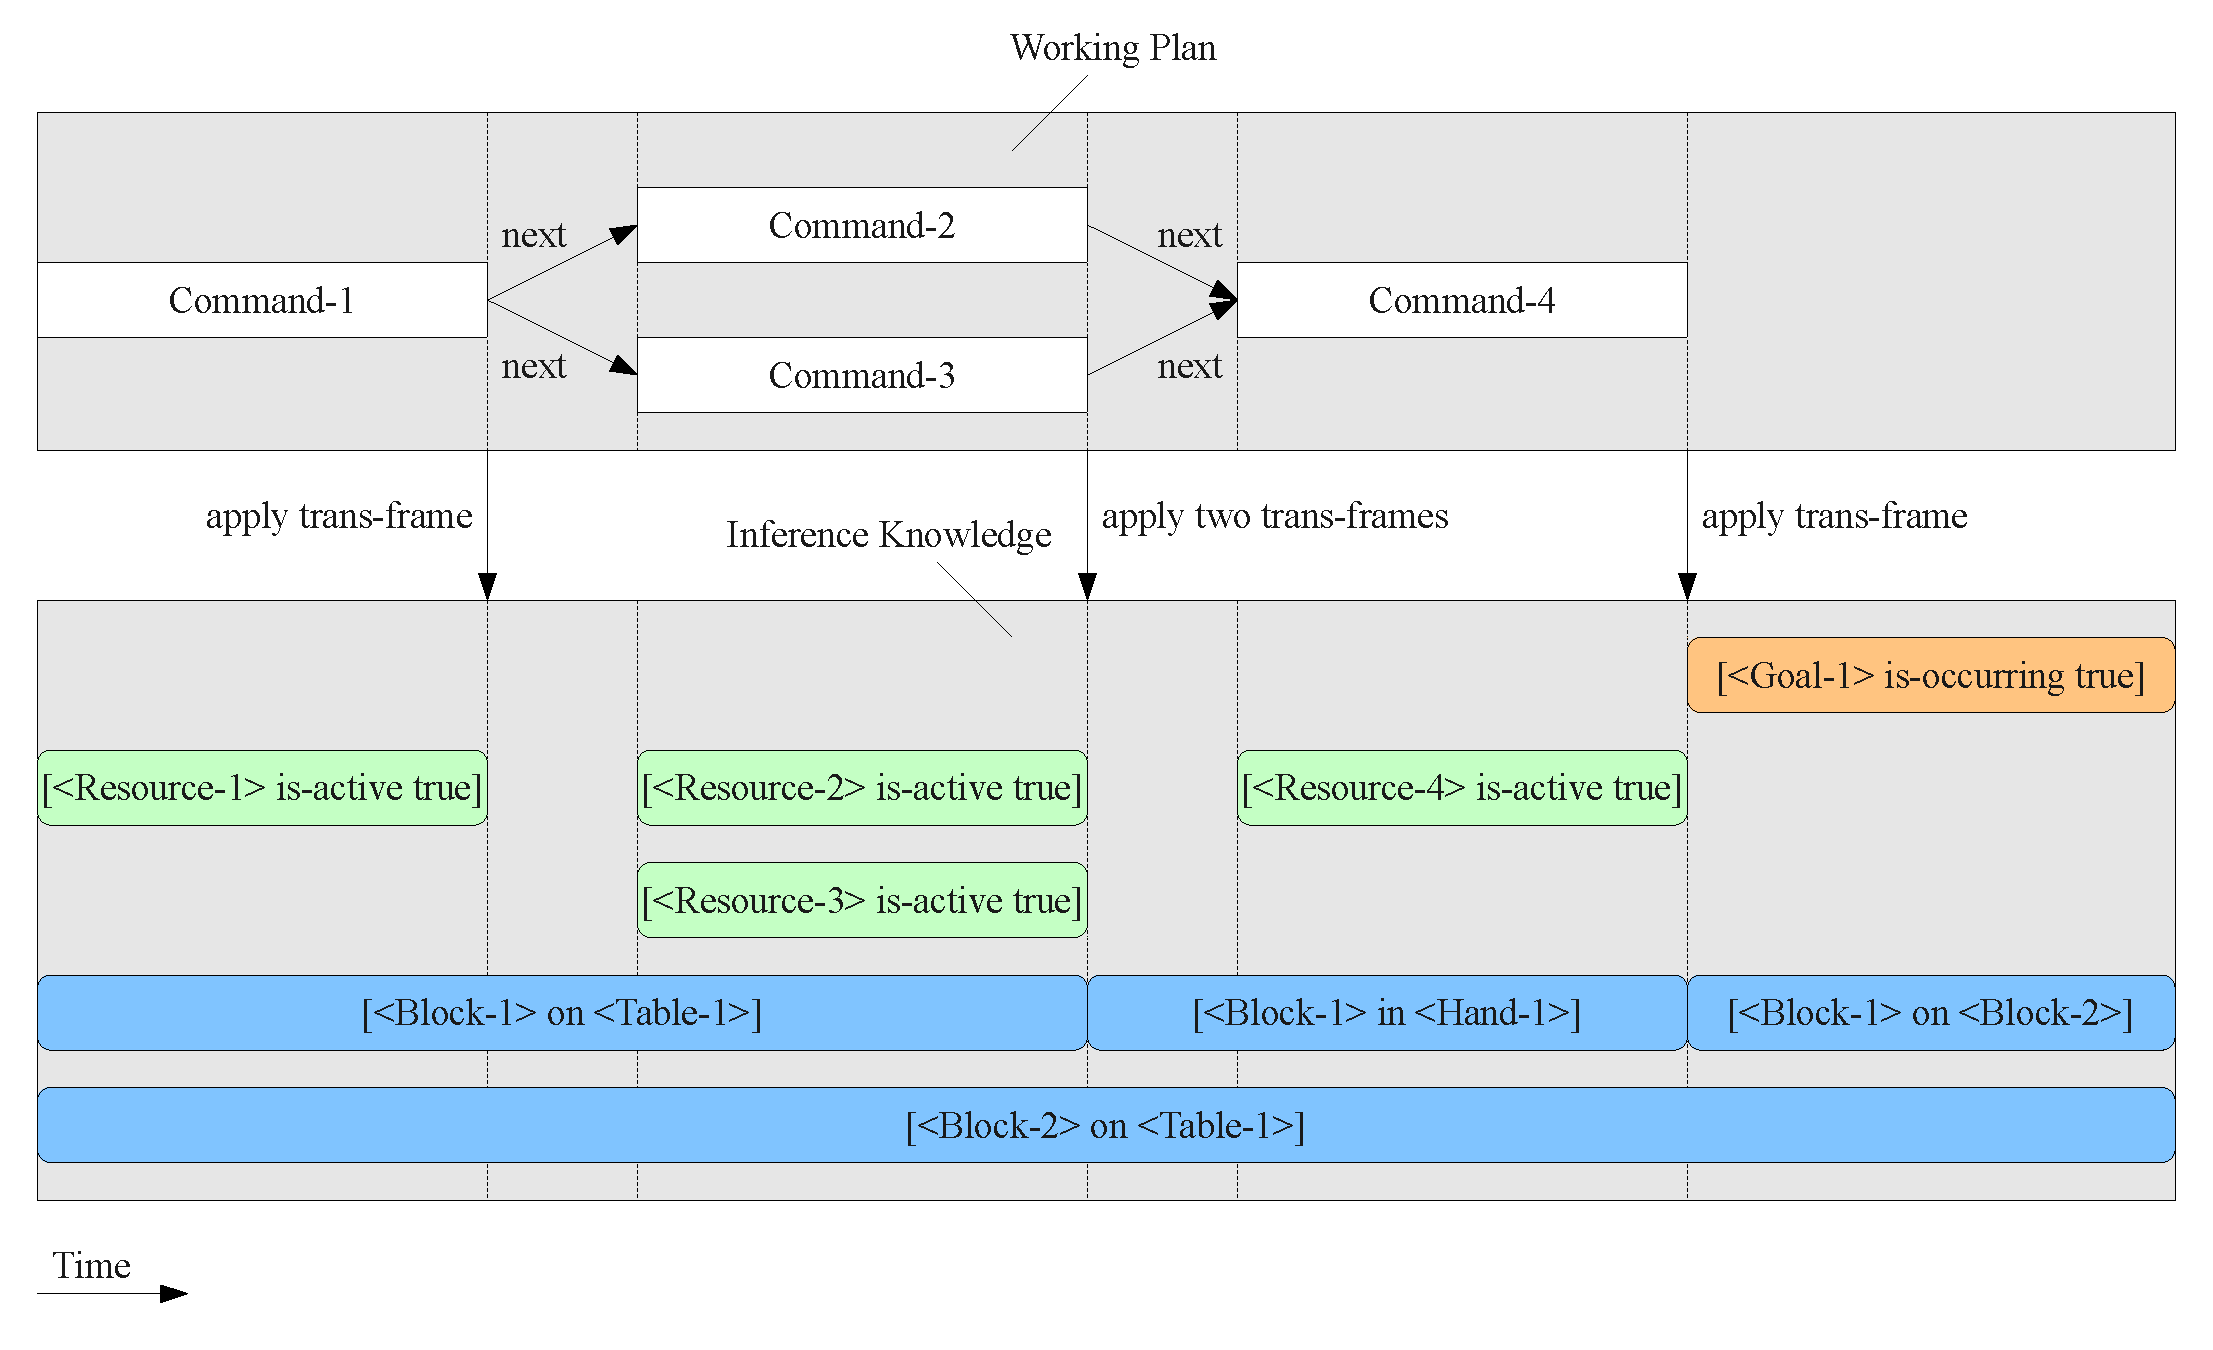
\includegraphics[width=11cm]{gfx/infer_plan_effects}
  \caption[Inferring the effects of a plan]{Inferring the effects of
    a plan.}
  \label{fig:infer_plan_effects}
\end{figure}

The planning process requires an inference algorithm to infer future
and past states based on cause-effect relationships between reflective
knowledge and physical knowledge.  Figure~\ref{fig:infer_plan_effects}
shows a possible inference for a given plan.  There are many ways to
plan and the specific planning system that I have implemented for my
experiments is discussed further in
Section~\ref{sec:details_of_inferring_the_effects_of_a_plan}.


\section{Planning Machine Operations}

\begin{figure}[bth]
  \center
  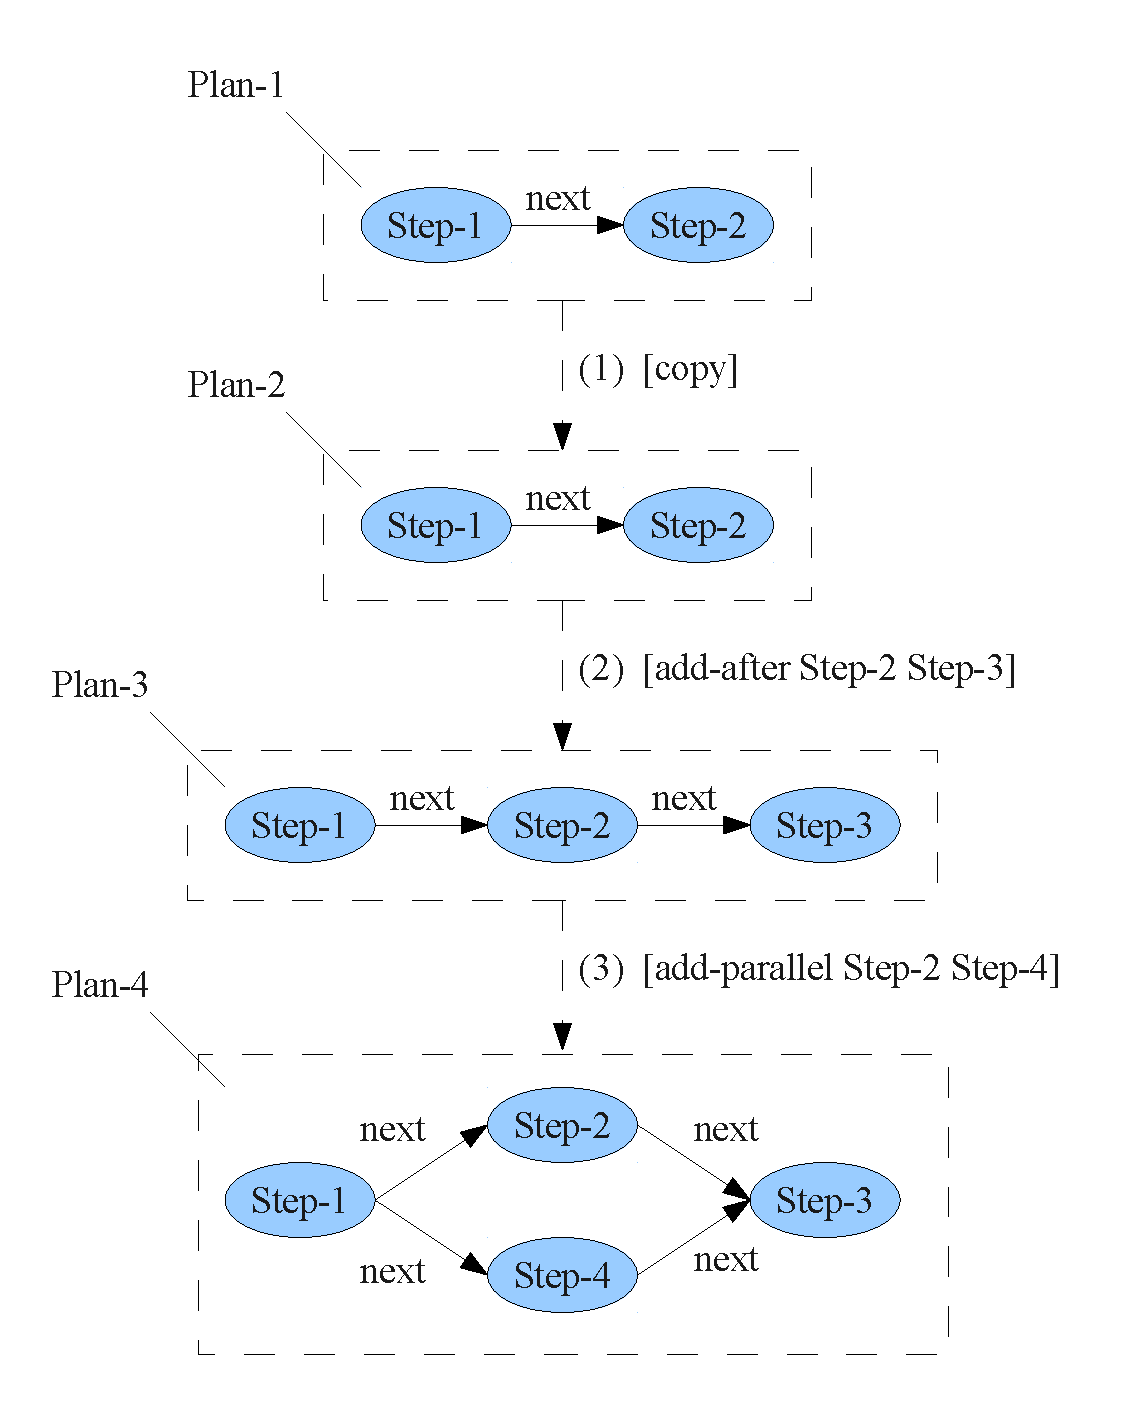
\includegraphics[height=8cm]{gfx/planning_machine_operations}
  \caption[A few planning machine operations]{A few planning machine operations.}
  \label{fig:planning_machine_operations}
\end{figure}

A few operations for manupulating partially-ordered plans are shown in
Figure~\ref{fig:planning_machine_operations}.


\section{Planning Machine Reflective Knowledge}

\begin{figure}[bth]
  \center
  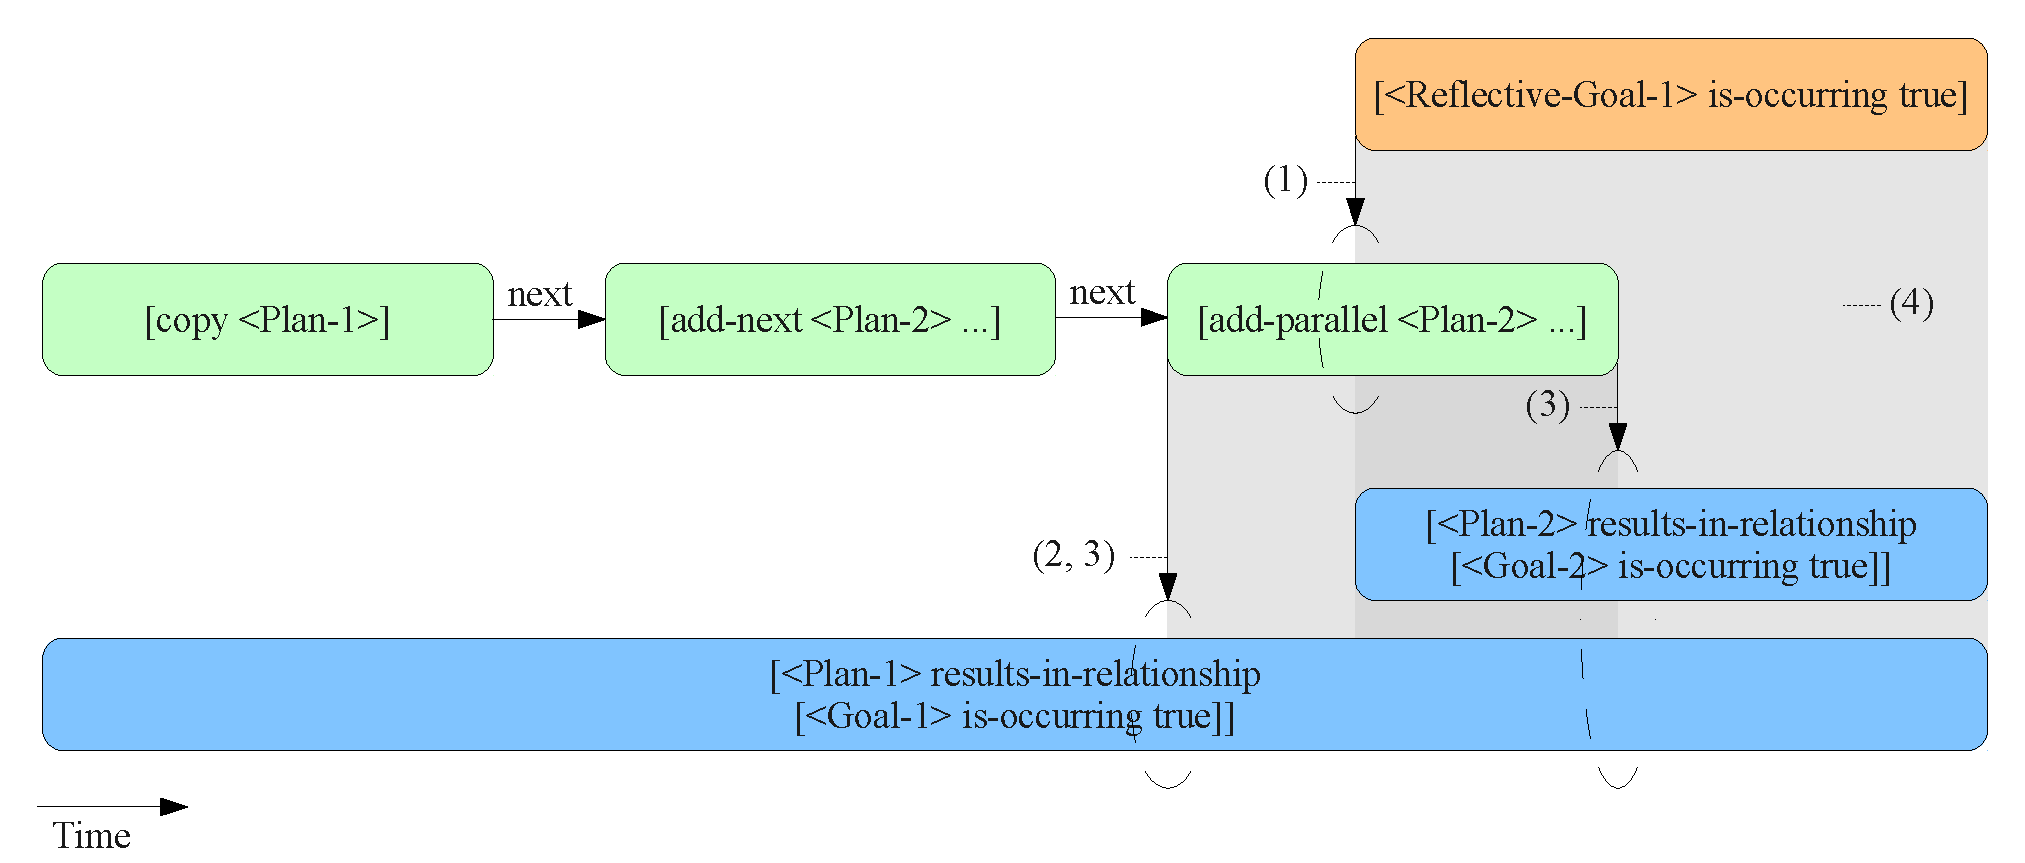
\includegraphics[width=11cm]{gfx/planning_machine_reflective_knowledge}
  \caption[Planning machine reflective knowledge]{Planning machine reflective knowledge.}
  \label{fig:planning_machine_reflective_knowledge}
\end{figure}

See Figure~\ref{fig:planning_machine_reflective_knowledge}.


%%************************************************
\chapter{Problems to Solve}\label{ch:problems_to_solve}
%************************************************

\section{Build a Reflective Knowledge Substrate}

The assumption that I introduced in
Section~\ref{sec:introducing_reflection_early_in_the_process},
``Introducing Reflection Early in the Process'', requires that changes
in my knowledge representation can be traced and compiled into other
representations, such as the reflective event representations used in
learning to accomplish goals.

\subsection{Automatic Collection of Audit Trails for All Processes}

Audit trails must be collected so that after the fact the events that
any process is resposible for can be used for many types of reflective
control purposes, such as learning to plan.  Although a system that
keeps track of everything that it does would support reflection, the
audit trail recorder in a system that does not grow indefinitely in
memory consumption would have options for focusing the collection of
audit trails, while also allowing for their garbage collection when
they are no longer needed by another reflective process.

\subsection{General Parallelism and Concurrency}

\begin{figure}[bth]
  \center
  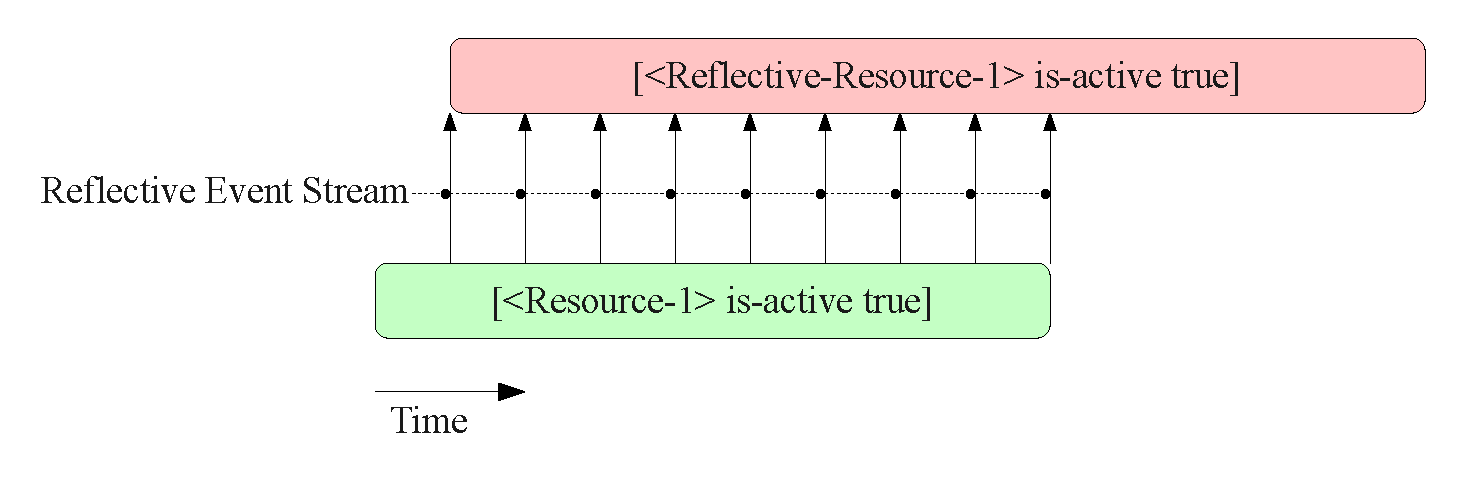
\includegraphics[width=11cm]{gfx/concurrent_parallel_reflection_efficiency}
  \caption[Concurrent parallel reflection efficiency]{Concurrent parallel reflection efficiency.}
  \label{fig:concurrent_parallel_reflection_efficiency}
\end{figure}

Because the procedurally reflective programming paradigm focuses on
event streams of changes to memory, there is an inherent ability to
express procedurally reflective algorithms in a streaming parallel
language.

Figure~\ref{fig:concurrent_parallel_reflection_efficiency} shows how a
simple process can be reflectively monitored without slowing down the
fundamental process by more than the constant time factor necessary
for generating the event stream.  Many different parallel reflective
processes can be reflectively processed concurrently without any
additional slowdown in the primary problem solving process.

\subsection{Program as Data}

The ability for a process to manipulate a program as data makes it
easier for that process or a user to read, edit, and write programs as
they are debugged.  The ability to change the functionality of a
program at run-time is a key component to creating an adaptive problem
solver.  Because of this, a programming language with a run-time
compiler is very useful for building these types of adaptive systems
that learn to debug and re-program their own subprograms.  For purely
the reason of developing problem solving learning algorithms, it is
critical that a reflective substrate has the ability to treat its own
programs as data.


\section{Layered Reflective Problem Solving}

\subsection{Analogy between Physical Goals and Planning Goals}


\section{Learning by Credit Assignment}

\subsection{Use Reflective Representations for Better Models of Learning}

\subsection{Tracing Knowledge Provenance for Credit Assignment of Success or Failure}




%%*****************************************
\chapter{Theory and Alternatives}\label{ch:theory_and_alternatives}
%*****************************************

\section{Two Popular Approaches to Modelling Intelligence}

Recently, there have been two directions of research with the goal of
building a machine that explains intelligent human behavior.  The
first approach is to build a baby-machine that learns from scratch to
accomplish goals through interactions with its environment.  The
second approach is to give the machine an abundance of knowledge that
represents correct behavior.

Each of these solutions has benefits and drawbacks.  The baby-machine
approach is good for dealing with novel problems, but these problems
are necessarily simple because complex problems require a lot of
background knowledge.  The data abundance approach deals well with
complicated problems requiring a lot of background knowledge, but
fails to adapt to changing environments, for which the algorithm has
not already been trained.

\subsection{Adaptability in Complex Environments}

\begin{figure}[bth]
  \center
  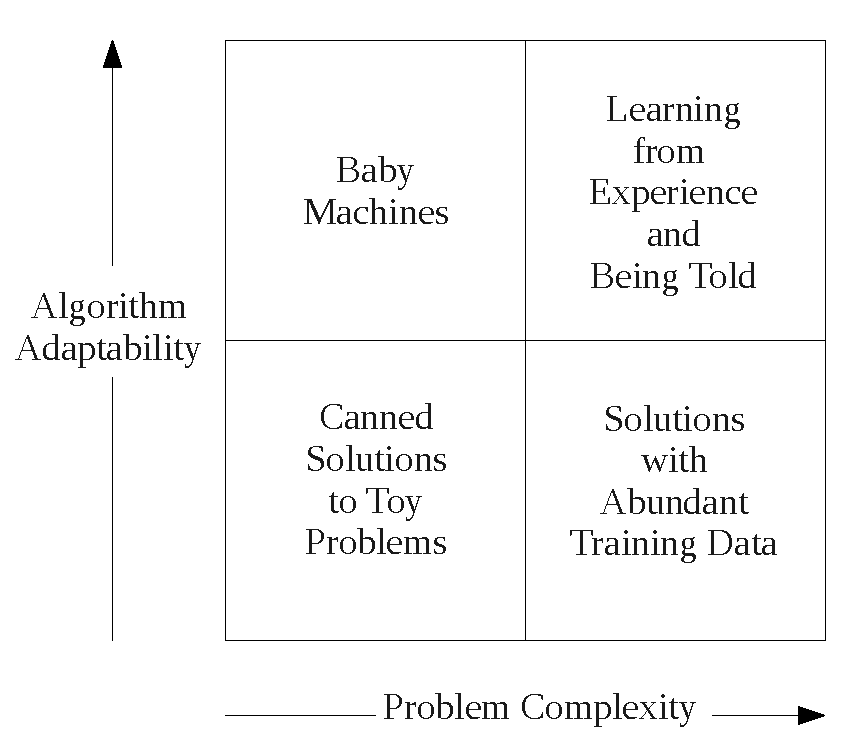
\includegraphics[height=6cm]{gfx/problem_complexity_versus_algorithm_adaptability}
  \caption[Problem complexity versus algorithm adaptability]{Problem
    complexity versus algorithm adaptability.}
  \label{fig:problem_complexity_versus_algorithm_adaptability}
\end{figure}

We would like to build intelligent machines that are able to perform
household tasks, such as cooking, cleaning, and doing the laundry, but
these tasks seem insurmountably complex, containing organically
unpredictable events.  We would like our machines to expertly handle
these extremely complicated problems, and we would also like them to
adapt to learn in unexpected or novel situations.  One popular
approach to building a machine that performs complicated tasks is to
give the machine a large training dataset that details every possible
situation that the machine may find itself within, along with the
correct action in that situation.  This is the so-called
``supervised'' learning approach.  These algorithms do not adapt to
novel situations well, and collecting these datasets is often
impossible for many problems, such as cooking and cleaning because it
is too difficult to enumerate all possible situations, in which the
machine may find itself.  Also, if the machine is cooking a meal, we
would like to be able to explain an idea for a new recipe to the
machine, or to perhaps be a partner in discovering new recipes, or we
may simply want to explain to the machine that a guest has a specific
allergy to walnuts, making that ingredient an exception for this meal
but not others.
Figure~\ref{fig:problem_complexity_versus_algorithm_adaptability}
shows how problem complexity and algorithm adaptability can be thought
of as a two-dimensional space into which different algorithmic
approaches can be used as solutions.

\subsection{The Abundant Data Approach}

There have been many approaches to modelling complex forms of
reasoning by collecting large amounts of knowledge that describes
correct or acceptable behavior in a domain.  For example, there are
examples of complex multi-agent commonsense simulation environments
collects thousands of examples of users interacting in a complicated
object-oriented social simulation \citep{orkin:2009},
\citep{orkin:2010}.  These systems have complicated domains, but these
projects do not attempt to build agents that attempt to accomplish
goals.  Instead, these systems are inference systems that simply try
to reproduce typical behavior, rather than goal-directed behavior.

There are many commonsense reasoning systems that do not interact with
simulation environments at all, but which attempt to demonstrate
commonsense reasoning by being told large amounts of knowledge.  The
Cyc project is one large such project that has been told large amounts
of logical knowledge \citep{lenat:1990}.  There is also effort
directed toward populating Cyc with knowledge automatically gathered
from the web \citep{matuszek:2005}.  The OpenMind project
\citep{singh:2002} is a project that gathers large amounts of
approximately correct commonsense knowledge from people online.  The
OpenMind knowledge has been turned into many inference systems that
can compare and generate new commonsense knowledge \citep{liu:2004a,
  liu:2004b, speer:2009}.

\subsection{The Common Sense Reasoning Problem Domain}

Common sense is the set of common reasoning abilities shared by most
people in a given social group.  Another way to say this is that
common sense is the set of reasoning abilities that one would assume
of a typical person that they meet for the first time and know nothing
about.  For example, most people have a naive theory of physics, so
you would expect someone to know that things fall when they are not
supported and liquids flow or are absorbed unless they are in a
container.  Common sense relies on a lot of knowledge that is assumed
that most everyone knows.

%TS>> what is a given social group... i share very little reasoning abiltities about user TS>>interface with my daughter or the director of CMU Siliicon Valley or my bike riding 
%TS>> friends, or my brothers,....

%TS>> not crisp enough ... a person is not defined as a person...but realtive to a 
%TS>> role we have with them,,, a mechanic talks differently to a woman or man, a professor
%TS>> or his accountant about cars 

%TS>> again, people have different theories of physics than each other 

%TS>> i have been served food in which the floating stuff  was designed to change through 
%TS>> the period of servign and eating soup  ..

%TS>> I am ready for  a fight on that , i live with a woman, a teenage girl, an autistic,
%TS>> my neighbor is a morman, the woman next door is totally rich... very diffferent 
%TS>> world views... even about how to deal with trash from a dinner. 

%TS>> I don't know what YOU mean by common sense yet,,,, define something specific
%TS>> does it cover diffferent minds or clones, what about its edges,   


Building a machine that demonstrates common sense reasoning is a
long-standing goal of the field of artificial intelligence.  One of
the difficulties in developing algorithms for dealing with a common
sense reasoning domain is that the algorithm needs a lot of background
knowledge about a given domain before it can answer even simple
questions about it.  However, this knowledge is often only true in
very specific situations and has many exceptional cases.  For example,
the knowledge that most birds can fly is generally true, but we also
know that many birds are flightless, such as penguins, ostriches, and
road runners.  Also, we have knowledge about the typical behavior of
objects; for example, we know that refrigerators keep things cold,
but we also reason efficiently about exceptional cases, such as when
the refrigerator is not plugged in, or when the power goes out.

%TS>> yes but those are examples we have seen for decades with varying 
%TS>> logical relations solving them
%TS>> show some that we haven't been able to do or places where you hold
%TS>> up where others have always been brittle 
%TS>> flexibility, integrity, hypocracy, intentionality changing belief systems...? 


\subsection{Representations for Common Sense Reasoning}

There have been many approaches to artificial intelligence that use
first-order logic as a representation for these types of knowledge and
their exceptions, but these systems become cumbersome in their
inability to express ``fuzzy'' sorts of relationships, such as when
the knowledge is applicable, for example the modifiers, ``most of the
time'', ``usually'', and ``almost never'', are difficult to express in
first-order logic.  When we have a lot of knowledge, we need ways to
keep track of in which situations this knowledge is useful.  This is a
form of ``meta-knowledge'', or knowledge about knowledge.
Meta-knowledge about first-order logic cannot be expressed in
first-order logic, so another type of representation is required for
this type of knowledge.  Therefore, we need other ways to represent
our knowledge in addition to logic.

\begin{quote}
``Nonetheless, theorem proving is in the worst case an intractable
  problem, even with no variables or unification, so no algorithm is
  going to work on the problem all the time. In this respect, theorem
  proving, for all its superficial formalism, is a lot like other
  branches of AI.  Where a theorist views a problem as solved if he
  has found an efficient algorithm or a discouraging lower bound, an
  AI researcher is often happy to find an algorithm that seems to work
  on some interesting problems, even though he doesn't really know the
  bounds of what it can do. Exploration will reveal the extent of its
  powers-each time it solves one more interesting problem something
  has been
  gained.''~---~\defcitealias{mcdermott:1987}{Drew~McDermott}\citetalias{mcdermott:1987}
\end{quote}


\section{Comparable Cognitive Architectures}

EM-ONE, Cyc, Icarus, ACT-r, Soar, and Prodigy are comparable cognitive
architectures to the one that I have built.

\subsection{The EM-ONE Cognitive Architecture}

I worked with Pushpinder Singh from 1999 to 2006 on the first version
of the Emotion Machine architecture, EM-ONE \citep{singh:2005}.
EM-ONE was an example of a reflective control system that used
commonsense stories in order to reason about social problem solving.
\cite{morgan:2009} discusses a number of things to learn from the
EM-ONE architecture that have informed my current approach.

Push and I have discussed that one weakness in the EM-ONE system is
its reliance on tracing only the declarative prolog statements, among
other necessary but untraced procedural code.  Although EM-ONE
contained a large amount of procedural knowledge, none of the effects
of this procedural knowledge could be debugged reflectively.  Toward
solving this problem, I have based my approach on a memory layer that
can trace the provenance of select memory events.

\subsection{Icarus}

Icarus is a cognitive architecture that supports a form of far
transfer learning \citep{konik:2009}.  The Icarus system allows for a
goal-directed structure mapping learning process.  These structure
mappings that are learned in this goal-directed way, can be useful
forms of analogy that enables ``far'' transfer in a cognitive system.
The Icarus work builds upon a previous model for analogical transfer
learning between symbolic relational structures \citep{gentner:1983}.

Because my knowledge representation is relational and symbolic, I see
Icarus' approaches to far transfer learning as highly compatible with
my architecture's ability to support multiple knowledge domains for a
single goal-oriented problem solving agent.  I am also interested in a
technique of using differences of differences \citep{winston:1970} as
an alternative to the structure mapping form of analogical transfer.

The Icarus system has also been applied to moral reasoning tasks in
order to build a theory of moral reasoning in humans \citep{iba:2011}.
I see similar applications of my architecture to these social
reasoning domains, but my planned approach to this domain is based on
two more layers of reflective control than I have currently
implemented \citep{morgan:2011}.

\subsection{Computational Models of Cognition about Cognition}

\cite{cox:2005} gives a good overview of the cognitive sciences that
deal with the problem of thinking about thinking, or
metacognition.

\subsection{Shades of Belief as Debugging Meta-Knowledge}

\cite{stein:1995} applies a prototype system to perform reflective
case-based reasoning over shades of beliefs in knowledge.

\section{Bounded Rationality}

There is an approach of economics and game theory that is called
bounded rationality \citep{simon:1972}.  These models deal with the
time constraints of not only acting efficiently in a domain but also
in optimizing the planning actions involved in accomplishing goals.
This approach assumes that there is an absolute numerical reward value
for accomplishing goals.  In the sense that absolute values for all of
the goals of a system are seldom known in practice, the bounded
rationality approach is limited in a general sense similar to the
simpler reinforcement learning approach.

\subsection{Feedback Control Model for Accomplishing a Single Goal}

\begin{figure}[bth]
  \center
  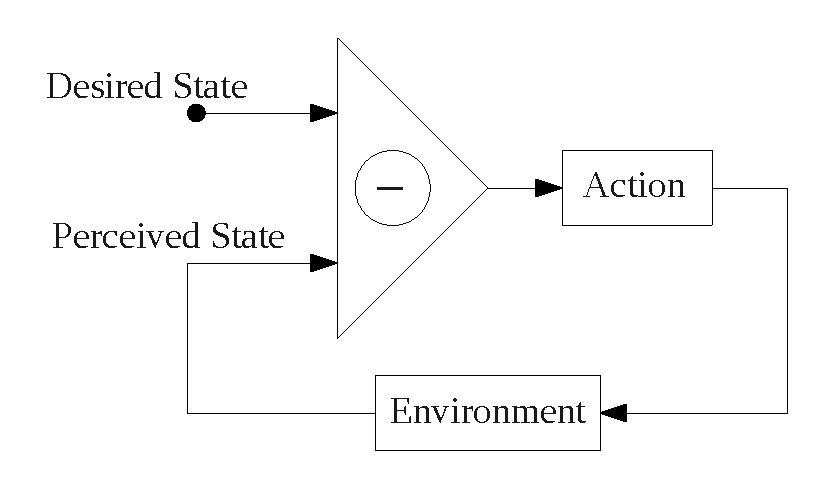
\includegraphics[width=6cm]{gfx/feedback_control}
  \caption[The feedback control model for accomplishing a single goal]{The feedback control model for accomplishing a single goal.}
  \label{fig:feedback_control}
\end{figure}

Now that we have discussed the basic model of learning from experience
what good goal states may be from rewards, let us consider the
representations for the state space of the perceptions and actions of
my model.  Control theory has given us many useful models for agents
that control continuous environments.  For example,
Figure~\ref{fig:feedback_control} shows a simple difference feedback
control circuit that is used in simple linear control systems.  The
system is given a desired state, there is a difference device that
calculates the difference between the actual perceived value from the
environment, and the control system then executes an action based on
that difference, which affects the environment.  The result in such a
negative feedback loop is that the agent's perception of the
environment is closer to the desired state.

\subsection{Means-End Analysis}

In 1959, Newell, Shaw, and Simon published a report on a means-end
analysis model that was designed to solve any symbolically represented
problem \citep{newell:1959}.  Their system was called the \ac{GPS},
and worked by being able to work with relational representations of
current and desired states.  The agent had a catalogue of differences
between states that it knew how to minimize.  The system worked by
finding the largest difference and executing the associated method for
reducing this difference.  This work has grown into the Soar model
\citep{newell:1990} for better solving symbolic planning problems, and
dealing with impasses for when the planning search runs out of
options.

\subsection{Difference-Engine Model for Accomplishing Multiple Goals}

\begin{figure}[bth]
  \center
  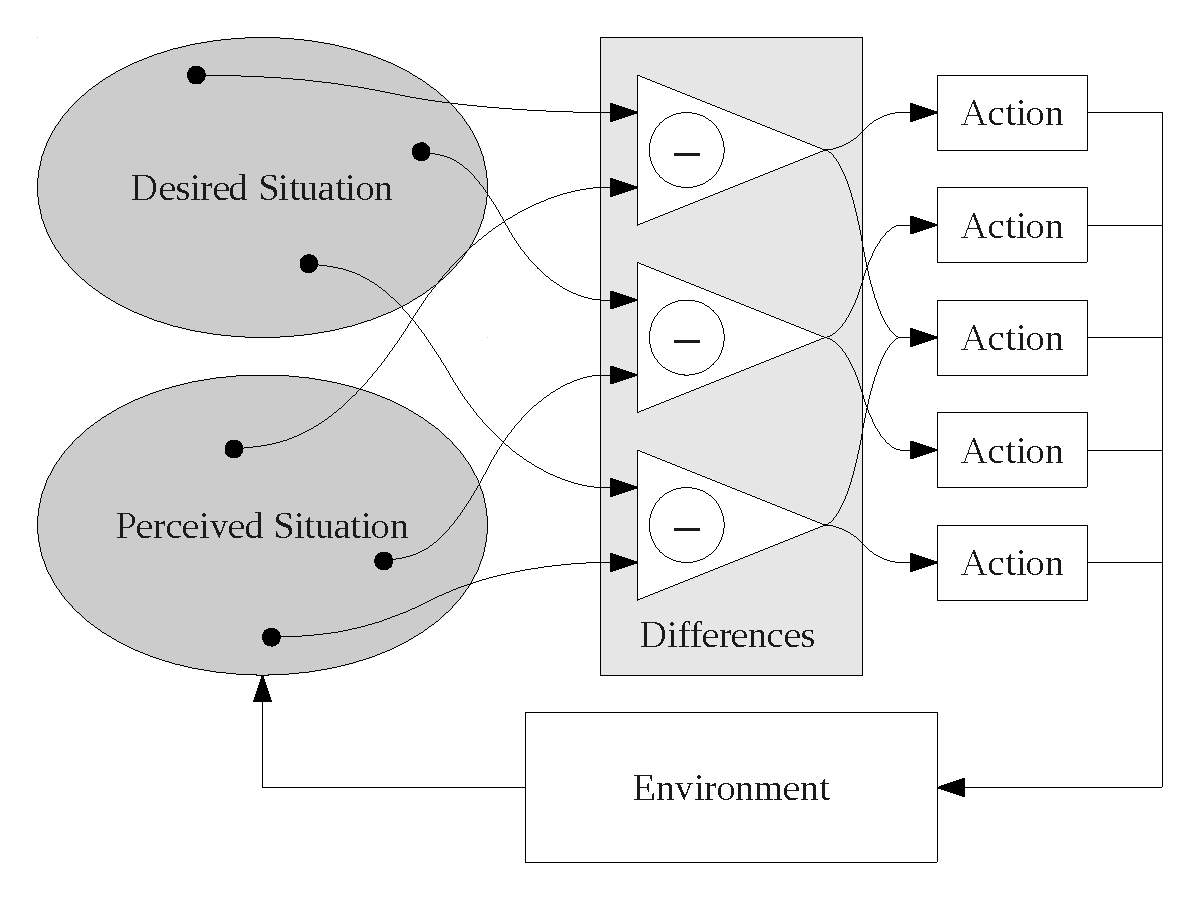
\includegraphics[height=6cm]{gfx/difference_engine_feedback_control}
  \caption[The difference engine model for accomplishing multiple goals]{The difference engine model for accomplishing multiple goals.}
  \label{fig:difference_engine_feedback_control}
\end{figure}

\citep[p.~78]{minsky:1988}



\section{Planning}

\subsection{Assuming a Correct Model of Environment}

There are many types of processes that make plans for accomplishing
goals, which make plans assuming a model of how actions theoretically
affect the environment.  These processes are called planners when they
create a representation for how actions should be performed,
potentially including temporal ordering constraints.

Planners are a specific part of a complete learning system, but the
primary function of a planner is to find a theoretical solution to a
given problem.  This theoretical solution, or plan, may be executed
and may fail or succeed, in accordance with the initial intentions for
executing the plan, the initial intentions for imagining the plan, or
any other intentions.  If the plan fails, then we may find something
to be modified in my knowledge in order to help us in avoiding this
failure next time.  The planning process is a small part of the
complete closed-loop learning algorithm that learns to plan from
experience with the environment and other agents.



If we are thinking about the temporal constraints of the problem
solving process itself, then we need to consider a reflective approach
to this control problem.

  , (1) the model of the cause-effect relationship
between actions and the world, (2) the model of cause-effect
relationships between planning actions and the creation of successful
plans.

\subsection{Declarative Programming, Logical Reasoning}


\section{Machine Learning}

One encompassing goal of the field of machine learning is to develop
systems that can accomplish goals.

For example, a Markov Decision Process contains a transfer function,
which is basically a combinational device.

Of course, this combinational device would get more complicated if I added probability.



\subsection{Why Did I Forget to Include Probability in my Theory?}



\subsection{The Reinforcement Learning Model}

\begin{figure}[bth]
  \center
  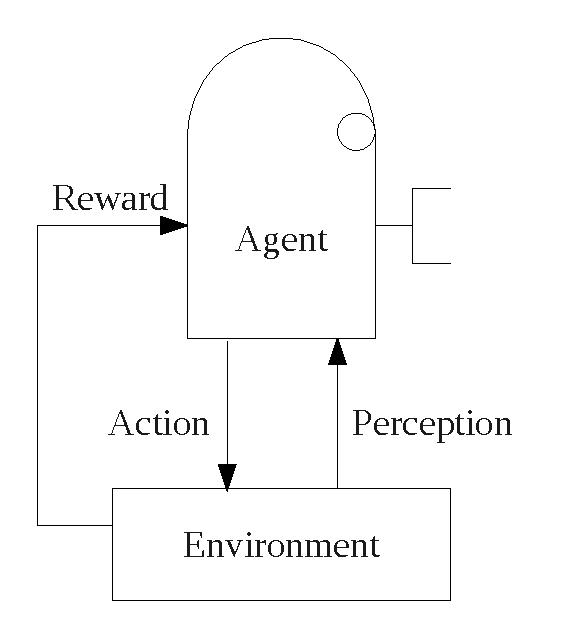
\includegraphics[height=5cm]{gfx/reinforcement_learning}
  \caption[The reinforcement learning model]{The reinforcement learning model.}
  \label{fig:reinforcement_learning}
\end{figure}

Figure~\ref{fig:reinforcement_learning} shows the basic reinforcement
learning model.  This model is an agent environment model, but there
is an extra information channel from the environment to the agent,
which communicates a numerical reward signal.  We can now say that the
agent has a learning problem.  The agent must learn what actions to
execute in order to gather the most reward.

\begin{figure}[bth]
  \center
  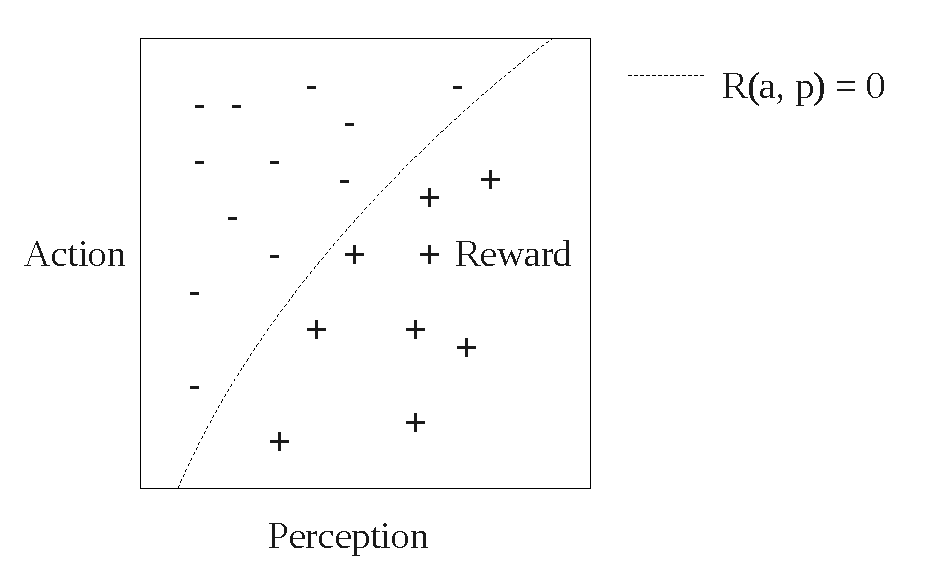
\includegraphics[height=4cm]{gfx/perception_categorization}
  \caption[Categorizing perceptions and actions based on goals]{Categorizing perceptions and actions based on goals.}
  \label{fig:perception_categorization}
\end{figure}

Once we have a basic reinforcement learning algorithm, we can approach
this learning problem as a function approximation problem.  In other
words, we can try to learn what parts of the perception and action
space have more or less reward.
Figure~\ref{fig:perception_categorization} shows a diagram of this
state space with the zero crossing of an approximation of the reward
plotted.

\subsection{Finding a Good Policy for Gathering Rewards}

Learning an approximation of what parts of a state space are good or
bad, based on reward, is not all that is needed to determine what
actions the agent should perform.  The agent wants to gather the most
rewards over time.  A simple way to formalize this problem is to learn
a policy that determines what action should be executed for every part
of the state space, based on some sort of summation of rewards over
time.  There have a been a number of ways of formalizing this
summation process as finite or infinite horizon problems
\citep{sutton:1998}.  Dynamic programming can be used for finding an
optimal or an approximately optimal policy \citep{bertsekas:1995}.

\subsection{Categorizing Perceptions and Actions based on Goals}

One problem with the reinforcement learning approach is that the only
representation of success or failure is a single number, the reward.
The basic reinforcement learning problem has been defined for finite
propositional state spaces.

A representation called \ac{RMDP} has been proposed
\citep{guestrin:2003} in order to extend reinforcement learning to
larger relational problem domains, but this method only focuses on an
object-oriented reward that does not have any global feedback about
the overall value of the situation.


\section{Philosophy}

\subsection{The Objective Modelling Assumption}

\begin{figure}[bth]
  \center
  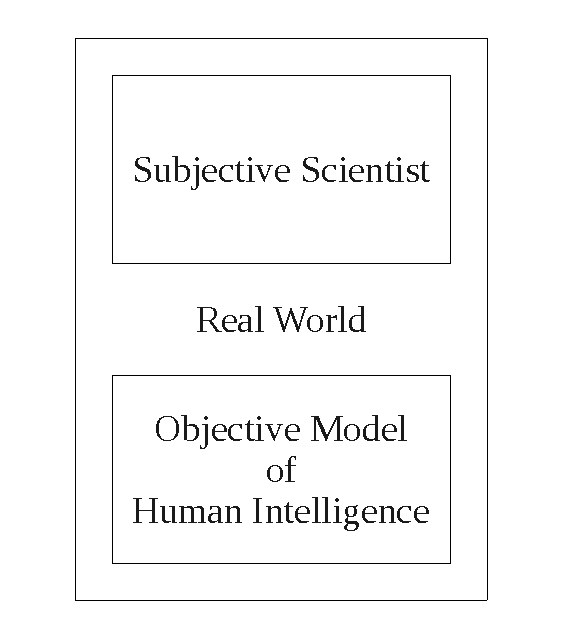
\includegraphics[width=4cm]{gfx/objective_description}
  \caption[The objective-subjective modelling assumption]{The objective-subjective modelling assumption.}
  \label{fig:objective_description}
\end{figure}

We assume that the phenomenon that we are trying to model, namely
human intelligence, is an objective process that we can describe.
This is the objective-subjective philosophical assumption that is
inherent in any objective scientific hypothesis.  We make this
assumption in order to avoid logical problems of circular causality
that occur when trying to find a non-objective description of
reflective thinking.  Figure~\ref{fig:objective_description} shows
how, given the objective assumption, the subjective scientist is part
of the real world, while she is studying an objective phenomenon.
Given the objective-subjective assumption, it would be a grave mistake
to confuse an objective model for reality itself.

\subsection{Being, Time, and the Verb-Gerund Relationship}

\subsection{The intensional stance}

\subsection{Reflective Representations}

\citep{perner:1991}


\section{Cognitive Science}


\subsection{The Development of Self-Conscious Emotions}

Between the ages of 1-3 years old, children display primary emotions,
such as joy, disappointment, and surprise.  These emotional processes
have been hypothesized to be related to the process of failing or
succeeding to accomplish a goal.  Around age 4, children begin to
display emotions that involve the self, such as guilt and shame.  It
has been hypothesized that these emotions relate to another person's
evaluation of the child's goals as good or bad.

We approach modelling this developmental process by applying Marvin
Minsky's theory of the child-imprimer relationship.  According to
Minsky's theory, at a young age, a human child becomes attached to a
person that functions as a teacher.  The imprimer could be a parent or
a caregiver or another person in the child's life, but the function of
the imprimer is to provide feedback to the child in terms of what
goals are good or bad for the child to pursue.

\subsection{Simulation Theory of Mind versus Theory Theory of Mind}


\subsection{Emotion or affect versus goal-oriented cognition}


\subsection{Embarrassment, Guilt, and Shame}



\section{Neuroscience}

\subsection{Neural Correlates of Consciousness}

\subsection{Learning by Positive and Negative Reinforcement}










\chapter{Related Background Research}
\label{other_models-chapter}

\section{The Layered ``Model-6'' Theory for Organizing Reflective Models}

Because the many fields of human cognitive modelling are so disparate
it is difficult to see them as a whole.  We are inspired by a layered
organizational scheme first presented in \cite{minsky:2006}.  The
six layers in this ``Model-6'' organizational scheme are named as
follows:

\begin{enumerate}
\item{Instinctive Reactions}
\item{Learned Reactions}
\item{Deliberative Thinking}
\item{Reflective Thinking}
\item{Self-Reflective Thinking}
\item{Self-Conscious Reflection}
\end{enumerate}

We hope that the reader will see that this is a useful way of organizing the massive amount of work that has gone into the computational modelling of abstract human thought processes since the conception of the field of artificial intelligence in 1956.
We are not claiming any biological correlations for these layers, but we are very excited by this unexplored possibility!
First, we must build such a model before any such statistical correlations could be found!
We see medical applications, such as categorizing spectrum mental disorders, as the highest-level goal in our work.

\subsection{Instinctive Reactions---Models of Insulation and Interaction}

\begin{quotation}
  \emph{We usually like to think in positive terms about how various parts of systems interact.}
  \emph{But to do that, we must first have good ideas about which aspects of a system do \emph{not} interact---since otherwise there would be too many possibilities to consider.}
  \emph{In other words, we have to understand \emph{insulations} before we can comprehend interactions.}
  \emph{To put this in a stronger form: \emph{No complicated society would actually work if it really depended on interactions among most of its parts}.}
  \emph{This is because any such system would be disabled by virtually any distortion, injury, or environmental fluctuation.}
  \emph{Nor could any such society evolve in the first place.}
\end{quotation}  

{\flushright{--- \cite{minsky:1988}}}

\subsubsection{Models of Failure in Distributed Systems}

\cite{attiya:2004} discuss algorithms for tolerating a few types of failures in distributed systems, ranging from silent crashes to arbitrary Byzantine failures, where parts of an algorithm perform in completely uncontrolled and unpredictable ways.
An algorithm for Byzantine tolerance is presented that is based upon building layers of first abstracting controllers that turn the Byzantine problem into a simpler \emph{identical Byzantine} problem.
The identical Byzantine problem is then abstracted to the simpler \emph{omission} problem, where a processor simply omits some messages from being transmitted.
The omission problem is then handled in a more abstract layer of the algorithm that when detecting an omission, crashes itself, resulting in a \emph{crash} problem.
Crash problems can be dealt in different ways for different algorithms, the simplest being the consensus algorithm.
This gives us a basic vocabulary of the most fundamental and basic distributed process problems.

\cite{bertsekas:1982} discuss a basic model for distributed dynamic programming that is organized around a distributed iterative approximation algorithm that computes a function mapping from states to values, $J(x){\in}\Re$.
His model divides the world into sets of states, $S_1 \cup S_2 \cup \cdots S_n = S$, that depend on neighboring sets of states in order to compute the approximation, $J^t$, of the optimal value function, $J^*$.
This fits with our abstract notion that commonsense knowledge in an artificial intelligence program should be organized according to what goals it is important to solve.
Having a basic optimal control theory of why this is a fundamentally sound organization principle is encouraging: perhaps organizing our knowledge by the values of goal states could also apply in the context of abstract reinforcement learning.
Note that the information theoretic organizational approaches such as the inductive logic approach used by relational reinforcement learning do not organize their knowledge according to which goal values are important for calculating which other goal values.

\subsubsection{Models of Uncontrolled Distributed Statistical Inference}
Recently, statistical propositional logic has become popular along with graph-based inference techniques for calculating both the most likely propositional state as well as the probability of any single propositional variable.
Statistical models are often represented in graphical form that can be easily distributed and computed by sparse matrix multiplication algorithms.
Given a statistical model, it is common to use the MAXENT algorithm to approximate the most likely state of such a model.
\cite{jaynes:1982} discuss when this may or may not be appropriate.
\cite{murphy:1999} discuss Pearl's ``loopy'' belief propagation algorithm which is an unreliable but efficient inference tool.
\cite{yedidia:2005} generalizes this distributed form of statistical inference to more powerful forms of hierarchical methods, explaining in the process that the forward-backward algorithm for hidden markov models, the Viterbi algorithm, Gallager's sum-product algorithm, the ``turbo-decoding'' algorithm, Pearl's ``belief propagation'' algorithm for inference on Bayesian networks, the ``Kalman filter'' for signal processing, and the ``transfer matrix'' approach in statistical mechanics are all of the same generalized form of statistical inference.

These statistical tools are the basic inference tools that claim nothing about their own applicability, and have no recourse for response for their own failures.
These statistical inference tools also know nothing about the goals which they are supposed to help solve.
In order for our algorithm to intelligently accomplish goals, we need to deliberate or plan our usage of these most basic tools.

\subsubsection{Models of Distributed Intelligence}

\cite{maes:1990} discuss learning to coordinate behavior, an argument for robust robot control using multiple ways of reasoning in a layered architecture.

\subsubsection{Models of Computational Reflection}

\cite{maes:1987} gives a great overview of ``computational reflection,'' which is basically keeping track of information about the execution of a program, so that other processes can use that information to better control the program.
Our approach to computational reflection is what they categorize as a ``frame-based'' approach, described first in \cite{minsky:1975} and first implemented in \cite{roberts:1977}.
\cite{maes:1987} describe the primary benefits of the frame-based approach as the following:

\begin{itemize}
\item{it helps the user cope with the complexity of a large system by providing documentation, history, and explanation facilities,}
\item{it keeps track of relations among representations, such as consistencies, dependencies and constraints,}
\item{it encapsulates the value of the data-item with a default-value, a form to compute it, etc.,}
\item{it guards the status and behavior of the data-item and activates procedures when specific events happen (e.g. the value becomes instantiated or changed).}
\end{itemize}

\cite{sobel:1996} discuss an introduction to reflection-oriented programming.
\cite{matsuoka:1992} discuss object-oriented concurrent reflective architectures.
\cite{oliva:1998} discuss the reflective architecture called ``Guaraná.''
\cite{watanabe:1989} discuss reflective computation in object-oriented concurrent systems.
\cite{yonezawa:1990} discuss a reflective object oriented concurrent language called ``ABCL/R.''
\cite{ancona:1998} discuss channel reification, which is a reflective model for distributed computation.
\cite{cazzola:1998} discuss evaluation of object-oriented reflective models.

\subsection{Learned Reactions---Models of Learning Reactions}

\subsubsection{Models of Planning to Perceive}

\cite{pryorcollins:1995} discuss how planning is used in perceptual processes.

\subsubsection{Models of Commonsense Reasoning}

There are many domains of quaitative commonsense reasoning, e.g. physics \cite[]{forbus:1994}, natural language \cite[]{liu:2004b}, story narratives \cite[]{williams:2005}, event planning \cite[]{smith:2006}, and psychology \cite[]{gordon:2008}.

\subsubsection{Models of Reactive Commonsense Knowledge}

There are also a few large knowledge bses of commonsense knowledge, e.g. ConceptNet \cite[]{liu:2004a}, FrameNet \cite[]{baker:1998}, Cyc \cite[]{lenat:1990}, AnalogySpace \cite[]{speer:2009}, and WordNet \cite[]{fellbaum:1998}.
Although these knowledge bases have a broad range of reasoning algorithms from linear algebraic semantic analogies in AnalogySpace to intricate microtheoretic logical deduction in Cyc, none of these knowledge bases are able to causal reflectively control the complexity of their algorithms.
Because commonsense knowledge is often represented in a declarative form, logical reasoning algorithms are often applied, but undirected logical reasoning methods often cannot handle large amounts of knowledge.
We hope that our causal reflective tools available in the Funk2 architecture will help in learning to reflectively control these explosive logical reasoning algorithms.
Another aspect that is critically important for organizing massive commonsense knowledge bases are goals; the knowledge should be indexed by types of goals.
We hope that our focus on goal-oriented learning in our reflective architecture will provide means of organizing learned knowledge in terms of the goals it is relevant for thinking about.

\subsection{Deliberative Thinking---Models of Learning to Compile Plans}

Artificial intelligence systems that use multi-step deliberation (or planning) in order to imagine hypothetical (counterfactual) sets of actions before executing these scripts (or plans) are implementing what is referred to as Layer 3 in the Emotion Machine theory of mind.

\cite{thagard:1995} discuss using a coherence theory of decision in order to perform inference to the best plan.
\cite{michalski:1995} discuss learning as goal-driven inference.

\subsubsection{Reinforcement Learning}

According to \cite{sutton:1998}, the field of reinforcement learning deals with the problem of ``learning what to do---how to map situations to actions---so as to maximize a numerical reward signal.''
Reinforcement learning is an online type of learning problem as opposed to supervised or unsupervised types of learning problems.

\cite{kaelbling:1996} gives a good overview of historical reinforcement learning.
The reinforcement learning problem is defined as

\begin{itemize}
\item{a set of states, $\mathcal{S}$,}
\item{a set of actions, $\mathcal{A}$, and}
\item{a set of scalar reinforcement signals, typically $\{0,1\}$ or $\Re$.}
\end{itemize}

It is interesting to consider how the well developed idea of ``exploration versus exploitation'' as discussed in \cite{kaelbling:1996} as a model for deciding when to sequentially meta-reason.

subsubsection{Models of Optimal Behavior}

\cite{kaelbling:1996} discuss three primary models of optimal behavior:

\begin{enumerate}
\item{the \emph{finite horizon} model in which an agent performs receding horizon control, such that total reward is $E(\sum_{t=0}^{h}{r_t})$,}
\item{the \emph{infinite discounted} model in which an agent uses future rewards discounted by a constant factor, $\gamma$, such that total reward is $E(\sum_{t=0}^{\infty}{\gamma^t r_t})$, and}
\item{the \emph{average reward} model which is the infinite limit of the finite horizon model, such that total reward is $\lim_{h{\rightarrow}\infty}{E(\frac{1}{h}\sum_{t=0}^{h}{r_t})}$.}
\end{enumerate}

Since we are dealing with modelling very large and complex systems, we see these optimality criteria as only applicable to small isolated aspects of the entire system.
Nonetheless, we hypothesize that useful approximations of optimal systems that can be derived from overlapping subsystems with constraining optimality criteria can be derived from these three basic types of optimality.
Homeostasis monitors and continual ``heartbeat'' controllers could be implemented with infinite or average optimality models, while short-term goal-oriented controllers would necessitate the complexities of the full $N$-step finite horizon model of optimality.

\subsubsection{Dynamic Programming and Optimal Control}

\cite{bertsekas:1995} describe techniques for finding optimal and approximate \emph{functional} (\emph{memoizable}) solutions to reinforcement learning control problems, using recursive formulas of flat state spaces that can be optimized very easily by using memoized functions.
While this approach does not handle abstract models of the agent's world, there are exciting options of combining a dynamic programming approach with an abstract form of reinforcement learning, such as the use of inductive logic described in \cite{dvzeroski:2001}.

\subsubsection{A Theoretical World Model}

A simple formulation of the reinforcement learning problem can be formulated in terms of Markov Decision Process (MDP) environments.
An MDP is defined as

\begin{itemize}
\item{a set of states, $\mathcal{S}$,}
\item{a set of actions, $\mathcal{A}$,}
\item{a reward function $\mathcal{R}:\mathcal{S}\times\mathcal{A}\rightarrow\Re$, and}
\item{a state transition function, $\mathcal{T}:\mathcal{S}\times\mathcal{A}\rightarrow\Pi{(\mathcal{S})}$.}
\end{itemize}

\subsubsection{Category Learning to Accomplish Goals}

Category learning in the context of goal-oriented problem-solving is an idea that is discussed by \cite{barsalou:1995}.

\subsubsection{Models of Learning by Positive or Negative Reward in the context of Relational Knowledge}

\cite{dvzeroski:2001} describe an interesting combination of inductive logic programming (ILP) \cite[]{muggleton:1992} and reinforcement learning.
The benefit of using abstract logical representations of propositional states, actions, and state values makes the basic reinforcement learning algorithm able to deal with relational state spaces, such as the blocks world toy problem and the other problem representations that we are focusing on in this PhD.
This form of learning abstractions takes a flat mental space and maps it to a hierarchical relational abstraction.

\subsection{Reflective Thinking---Models of Learning to Control Deliberation}

\subsubsection{Models of Commonsense Psychology}

Understanding human psychology in commonsense terms is an initiative described in \cite{gordon:2004}.
We see our work as building upon this development of a commonsense language for discussing the types of mental processes that humans have.
Also, \cite{gordon:2008} further develops this commonsense psychological language approach to describe the processes of self-reflection, which is even more relevant to our work.
The difference between our approach and the commonsense psychology approach is that our work simulates these mental processes in a computer, using the Funk2 causally reflective procedural programming language.
Previous approaches have represented psychological reasoning processes in a declarative logical form, but these logical forms cannot handle the large knowledge bases that are involved in general commonsense reasoning.

\cite{wilson:1977} discuss verbal reports on mental processes.
\cite{schank:1972} discuss primitive concepts underlying verbs of thought.

\subsubsection{Models of Unsticking Deliberation by Creative Analogical Thinking}

\cite{buchanan:1977} discuss creativity at the metalevel.
\cite{mueller:1990} discuss daydreamer.

A storytelling system that is called MINSTREL is discussed in \cite{turner:1994}; it is guided by creativity goals in order to develop good narratives.
The process of creative storytelling is handled very similarly to mechanical goal-oriented problem solving in this way.

\subsubsection{Models of Learning to Plan to Learn}

\cite{ram:1995a} discuss planning to learn.
\cite{desjardins:1995} discuss a decision-theoretic model for deciding what to learn next for accomplishing goals.
\cite{ram:1995b} discuss goal-driven learning in multistrategy reasoning and learning systems.
\cite{ram:1995c} discuss learning, goals, and learning goals.
\cite{cox:1999} discuss the construction of learning strategies in introspective multistrategy learning.

\subsubsection{Models of Learning by Credit Assignment through Temporal State Tracing}

\emph{Eligibility traces} are a simple reinforcement learning tool for temporal credit assignment for an agent entering positive and negative reward states.
For example, the \emph{backward} view of eligibility tracing as applied to the temporal difference, $\text{TD}(\lambda)$, learning method simply augments the basic learning algorithm with an additional eligibitity factor, $e_t(s)$, for each state.
Only non-zero values of the eligibility factor are remembered in tractible (approximate) implementations; this amounts to keeping a list of $n$ recently visited states.
In the algorithm, the current state's eligibility factor, $e_t(s_t)$, is set to $1$ and all other states are discounted by a constant eligibility discount factor, $\gamma$.
Credit assignment for rewards that are found in the world are assigned not only to the previous state, as in the basic one-step $\text{TD}(\lambda)$ algorithm but also assigned to the value functions in a discounted sense to the previous $n$ states in our eligibility trace.
We call this form of credit assignment ``Temporal State Tracing'' because it simply assigns credit to those states temporally local to the current state, i.e. there is no explicit consideration of causality involved in the assignment.

\subsubsection{Models of Learning by Credit Assignment through Causal Tracing of Failure}

We do not know of any reinforcement learning algorithms that reflectively learn how to plan through causal tracing of failures.
Our method of learning in this way is disussed in Section~\ref{causal_tracing_of_failure-section}.

\subsubsection{Models of Learning by Explaining Failures}

\cite{hammond:1990} discuss explaining and repairing plans that fail.
\cite{vanlehn:1992} discuss a model of the self-explanation effect.
\cite{ram:1995d} discuss introspective reasoning using meta-explanations for multistrategy learning.
\cite{leake:1995a} discuss goal-based explanation evaluation.
\cite{leake:1995b} discuss toward goal-driven integration of explanation and action.
\cite{dominowski:1998} discuss verbalization and problem solving.

\subsubsection{Models of Learning by Repairing Failed Plans and Inference Knowledge}

\cite{leake:1996} discuss learning to refine the case-based reasoning process through experience, introspection and expertise.
\cite{levin:2004} discuss how to span the difference between metacognitive failure and success in thinking about seeing.
\cite{cox:1996} discuss how to construct a learning strategy under reasoning failure in the terms of introspective multistrategy learning.

\subsubsection{The Difference between Metareasoning, Computational Reflection, and Causal Reflection}

\cite{hansen:2001} discuss a dynamic programming approach to monitoring and control of anytime algorithms.
\cite{cox:2007a} discuss metareasoning, monitoring, and self-explanation.
\cite{cox:2005} present a selected research review of metacognition in computation.
\cite{anderson:2007} present a review of recent research in metareasoning and metalearning.
\cite{cox:2007b} discuss perpetual self-aware cognitive agents.
\cite{cox:2008} present a manifesto on metareasoning.
\cite{davis:1980} discuss reasoning about control in terms of meta-rules.
\cite{fox:2001} discuss introspective reasoning for index refinement in case-based reasoning.
\cite{maes:1988} discuss issues in computational reflection.
\cite{minsky:1968} discuss matter, mind, and models.
\cite{newell:1982} discuss the knowledge level.

\subsubsection{Empirical Models of Reflective Thought}


\cite{baumeister:2007} discuss How emotion shapes behavior: Feedback, anticipation, and reflection, rather than direct causation.
\cite{vince:2002} discuss Organizing reflection.
\cite{mirvis:2008} discuss Executive Development Through Consciousness-Raising Experiences.
\cite{michalsky:2007} discuss Developing Students' Metacognitive Awareness in Asynchronous Learning Networks in Comparison to Face-to-Face Discussion Groups.
\cite{bivona:2008} discuss Executive function and metacognitive self-awareness after Severe Traumatic Brain Injury.
\cite{irannejad:2001} discuss The brain-mind cycle of reflection.
\cite{phillips:2005} discuss Self-awareness and the emotional consequences of self-discrepancies.
\cite{silvia:2006} discuss Emotion concepts and self-focused attention: Exploring parallel effects of emotional states and emotional knowledge.
\cite{lynn:2008} discuss The eq interview: finding employees with high emotional intelligence.


\subsection{Self-Reflective Thinking---Models of Control using Self and Other Models}

\cite{anderson:2005} discuss the metacognitive loop and the problem of brittleness in terms of logic, self-awareness and self-improvement.
\cite{schubert:2005} discuss some knowledge representation and reasoning requirements for self-awareness.

\subsubsection{Models Involving Multiple Agents}

Models of multiple intelligent agents that work together to solve problems have become popular in the field of machine learning called ``multi-agent reinforcement learning.''
Many popular surveys of the field exist \cite[]{wei:1995} \cite[]{sen:1999} \cite[]{stone:2000} \cite[]{shoham:2004} \cite[]{yang:2004} \cite[]{panait:2005}.

\cite{boutilier:1996} discuss a specific type of $n$-person cooperative game theory, in which agents share common goals, or in other words, a joint value function.
\cite{rapoport:2001} discuss $n$-person game theory in more detail.

\cite{bowling:2000} describe an analysis of stochastic game theory for multiagent reinforcement learning.
\cite{claus:1998} describe the dynamics of reinforcement learning in cooperative multiagent systems.
\cite{crites:1998} describe elevator group control using multiple reinforcement learning agents.
\cite{ghavamzadeh:2006} describe hierarchical multi-agent reinforcement learning.
\cite{guestrin:2002} describe coordinated reinforcement learning.
\cite{hu:1998} describe a theoretical framework and an algorithm for multiagent reinforcement learning.
\cite{kapetanakis:2002} describe reinforcement learning of coordination in cooperative multi-agent systems.
\cite{mataric:1997a} describe reinforcement learning in the multi-robot domain.
\cite{park:2001} describe modular $Q$-learning based multi-agent cooperation for robot soccer.
\cite{sandholm:1996} describe multiagent reinforcement learning in the iterated prisoner's dilemma.
\cite{tan:1997} describe independent versus cooperative agents in multi-agent reinforcement learning.
\cite{wang:2003} describe reinforcement learning to play an optimal Nash equilibrium in team Markov games.

\subsubsection{Multiagent Reinforcement Learning with Layered Models}
\cite{stone:1997} describe layered Learning in multiagent Systems.

\subsubsection{Multiagent Reinforcement Learning with Communication}

\cite{drogoul:1994} describe an application to social differentiation in ant colonies using a multi-agent simulation as a tool for modeling societies.
\cite{fischer:2004} describe hierarchical reinforcement learning in communication-mediated multiagent coordination.
\cite{price:1999} describe implicit imitation in multiagent reinforcement learning.
\cite{sen:1998} describe individual learning of coordination knowledge.

\subsubsection{Multiagent Reinforcement Learning with Self- and Other- Models}

\cite{mataric:1997b} describe learning social behavior.
\cite{nagayuki:2000} describe an approach based on the otheragent's internal model in multi-agent reinforcement learning.
\cite{noble:2004} describe social learning in a multi-agent system.
\cite{nowe:2001} describe social agents playing a periodical policy.

\subsubsection{Models of Parent and Child Social Functions}
\cite{castelfranchi:2001} describe the challenges for computational social science and multi-agent learning in a theory of social functions.


\subsubsection{Empirical Models of Inferring Person Traits}

\cite{asch:2005} discuss how impressions of personalities are formed.
They break personality down into $18$ two-part models, or dimensions (not necessarily independent).
These 18 dimensions are listed in the following table for reference:

\begin{tabular}{rll}
  1.         & generous           & ungenerous \\
  2.         & wise               & shrewd \\
  3.         & happy              & unhappy \\
  4.         & good-natured       & irritable \\
  5.         & humorous           & humorless \\
  6.         & sociable           & unsociable \\
  7.         & popular            & unpopular \\
  8.         & reliable           & unreliable \\
  9.         & important          & insignificant \\
  10.        & humane             & ruthless \\
  11.        & good-looking       & unattractive \\
  12.        & persistent         & unstable \\
  13.        & serious            & frivolous \\
  14.        & restrained         & talkative \\
  15.        & altruistic         & self-centered \\
  16.        & imaginative        & hard-headed \\
  17.        & strong             & weak \\
  18.        & honest             & dishonest \\
  \emph{19.} & \emph{warm}        & \emph{cold} \\
  \emph{20.} & \emph{intelligent} & ~ \\
  \emph{21.} & \emph{envious}     & ~
\end{tabular}	      

\cite{winter:2005} discuss the difference between \emph{dispositional} inferences and \emph{situational} inferences.
A dispositional statement is a statement about the relationship between person models, such as ``kind person'' or ``she helped the man'', whereas a situational statement is a statement that does not refer to such a model of a social relationship between person models, such as ``she dropped the groceries''.
Here is the list of 18 dispositional properties that they discovered in their research interviewing college students for word associations:

\begin{tabular}{rl}
  1. & generous          \\
  2. & rude              \\
  3. & good worker       \\
  4. & helpful           \\
  5. & ill-mannered      \\
  6. & thrifty           \\
  7. & talented          \\
  8. & bigot             \\
  9. & friendly          \\
  10. & concerned citizen \\
  11. & absent-minded     \\
  12. & kindhearted       \\
  13. & cheap             \\
  14. & clever            \\
  15. & inconsiderate     \\
  16. & willpower         \\
  17. & considerate       \\
  18. & clumsy
\end{tabular}

\subsubsection{Empirical Models of Self and Other Social Models}

This section discusses much research that often uses words that we often do not see used precisely.
For example, the phrase ``self-awareness'' is often used to describe a sort of mental process that monitors another mental process.
In this document, we try to be consistent by using the word ``self'' to only refer to models of self versus other in terms of agents thinking about personalities or properties of agents.
Other common uses of the terms ``self-awareness'' and ``self-consciousness'' are often less clear and refer to any kind of reflective process perceiving the execution of another process within the mind.
There are many forms of reflective thought, and we choose to use the term ``self-reflection'' to refer to those reflective processes that deal with self and other personality models of inter-agent relationships.

\cite{goverover2007tis} discuss treatment to improve self-awareness in persons with acquired brain injury.
\cite{baumeister1993etl} discuss when ego threats lead to self-regulation failure: negative consequences of high self-esteem.
\cite{gilbert2005ocb} discuss perceptions of people.
\cite{ross2005bispc} discuss social roles, social control, and biases in social-perception processes.
\cite{hobson2006sad} discuss self-awareness in developmental perspective.
\cite{hutchinson2007saa} discuss relationships among adaption-innovation, self-monitoring, and self-consciousness.
\cite{keenan2007crr} discuss the selective causal role of the right hemisphere in self-awareness.
\cite{morin2004lca} discuss a comparison and integration of various views of the levels of consciousness and self-awareness.
\cite{silverman2008osr} discuss self-reflection.
\cite{smith2007sap} discuss self-awareness, perspective-taking, and self-face recognition.
\cite{soeiro2008svtsf} discuss state versus trait self-focus: comparing self-awareness to self-consciousness.
\cite{uhlmann2008vsc} discuss varieties of social cognition.
\cite{burns1998scc} discuss individual selves, self-awareness, and reflectivity in the social construction of consciousness.
\cite{duval2002sap} discuss self-awareness, probability of improvement, and the self-serving bias.
\cite{focquaert2008ecn} discuss an evolutionary cognitive neuroscience perspective on human self-awareness and theory of mind.
\cite{whitehead2001sma} discuss social mirrors and shared experiential worlds.


\subsubsection{Empirical Models of Person Groups}

\cite{menon2005cacoa} discuss the attribution to individual versus group dispositions in culture and the construal of agency.

\subsection{Self-Conscious Reflection---Models of Learning by Imprimer Reflection on Self and Other Models}

\subsubsection{Empirical Models of Imprimers}

\cite{hinton2008rlsa} discuss The Role of Leader Self-Awareness in Building Trust and Improving Student Learning.
\cite{taylor2007cfetla} discuss A Conceptual Framework and Empirical Test for Leader Attunement: Toward a Theory of Leader Self-Awareness.
\cite{hare1993wc} describe Without Conscience: The Disturbing World of the Psychopaths Among Us.

\subsubsection{Moral Decisions and Values}

\cite{harsanyi1980rur} discuss rule utilitarianism, rights, obligations and the theory of rational behavior.
\cite{duval1999osa} discuss how changing self or changing standards of correctness also changes objective self-awareness and causal attributions for self-standard discrepancies.


\section{Natural Language in Problem-Solving}

\cite{bobrow1968nlicpss} discuss Natural Language Input for a Computer Problem-Solving System



\section{Models of Story and Language Understanding}


\cite{rammoorman1999toru} discuss understanding language understanding in terms of Toward a Theory of Reading and Understandin.
\cite{rapaport1999caf} discuss understanding language understanding in terms of Cognition and Fiction.
\cite{mahesh1999spiu} discuss understanding language understanding in terms of Sentence Processing in Understanding: Interaction and Integration of Knowledge Sources.
\cite{domeshek1999ctccn} discuss understanding language understanding in terms of Capturing the Contents of Complex Narratives.
\cite{ram1999toqqa} discuss understanding language understanding in terms of A Theory of Questions and Question Asking.
\cite{peterson1999sct} discuss understanding language understanding in terms of Semantic Correspondence Theory.
\cite{moorman1999crunc} discuss understanding language understanding in terms of Creativity in Reading: Understanding Novel Concepts.
\cite{coxram1999sual} discuss understanding language understanding in terms of On the Intersection of Story Understanding and Learning.
\cite{gerrig1999tpanw} discuss understanding language understanding in terms of Text Processing and Narrative Worlds.

\section{Evaluating Models of Complex Learning}


\subsection{Evaluating Models of Learning Skill Knowledge}
\cite{anderson1993alps} describe a model of complex learning about Acquisition of LISP Programming Skill.
\cite{ohlsson1993ibkpacs} describe a model of complex learning about The Interaction Between Knowledge and Practice in the Acquisition of Cognitive Skills.

\subsection{Evaluating Models of Learning by Self-Explanation}
\cite{vanlehn1993lbeeo} describe a model of complex learning about Learning by Explaining Examples to Oneself: A Computational Model.
\cite{kieras1993lsepe} describe a model of complex learning about Learning Schemas from Explanations in Practical Electronics.
\cite{rosenbloom1993bpebl} describe a model of complex learning about Bias in Planning and Explanation-Based Learning.

\subsection{Evaluating Models of Learning Declarative Relational Knowledge}
\cite{huffman1993cidt} describe a model of complex learning about Correcting Imperfect Domain Theories: A Knowledge-Level Analysis.
\cite{hammond1993csacbp} describe a model of complex learning about A Cognitive Science Approach to Case-Based Planning.
\cite{wilensky1993kanlp} describe a model of complex learning about Knowledge Acquisition and Natural Language Processing.

\subsection{Visual Programming Languages for Psycological Study of Complex Models}

\cite{cooper2002mhl} and \cite{cooper1998cvd} discuss how to model high-level cognitive processes in an empirical and scientific way.
Much of their work is presented in terms of their COGENT cognitive architecture that includes a visual programming language for cognitive scientists to quickly build and evaluate varieties of complex hypotheses.

\cite{cooper1995too} discuss an object-oriented language for cognitive modeling
\cite{cooper1996smc} discuss A systematic methodology for cognitive modelling
\cite{cooper1998ced} discuss COGENT: An environment for the development of cognitive models
\cite{councill2003esa} discuss Explaining Soar: Analysis of existing tools and user information requirements
\cite{mulholland1998hfc} discuss Hank: A friendly cognitive modelling language for psychology students
\cite{mulholland1999pph} discuss Programming with a purpose: Hank, gardening and schema theory
\cite{mulholland2000lbv} discuss Learning by building: A visual modelling language for psychology students
\cite{yule2001ttc} discuss Towards a technology for computational experimentation

\section{Models of the Large-scale Integration of Multiple Models of Cognition}

\cite{langley2008car} gives a good overview of the current state of the field of cognitive architectural design in terms of what exists and what needs to still be designed and built.
Among the features that are not much explored are the types reflective processes that control deliberative processes, which \cite{sloman2001vaa} refers to as meta-management.
We see building layers of these reflective management processes in the top three layers of the Emotion Machine theory as our basic inspiration for higher orders of reflective control beyond meta-management.

\subsection{The EM-ONE Model}

\cite{singh2005one} describe the first cognitive architecture based on the Emotion Machine theory of mind, developed in \cite{minsky2006em}.
This architecture includes the ability to control reasoning using a relational list commonsense narrative representation.
In terms of types of representations, the Emotion Machine theory proposes that self models exist in the self-reflective layer and imprimer models exist in the self-conscious layer.
Our purpose is to elaborate on this example model in a much larger and more powerful causally reflective programming language.
Our Funk2 architecture is based on procedural forms of run-time reflection that is built into the underlying programming language, whereas the previous work was based on declarative forms that used an assortment of programming languages, including Lisp and Prolog.

\subsection{The Icarus Model}

\cite{langley2005aap} describe an architecture that uses meta-knowledge of knowledge.
They refer to skill planning as planning toward long-term goals in the abstract meta-knowledge plan space.
They refer to short-term planning as planning over instances of the skill plans.
We see our approach as complimentary to this plan abstraction approach because we are focused on adaptive learning due to failures of conflicting plans, so we expect our approach to be adaptable to this form of meta-planning as well.

\subsection{The ACT-r Model}

\cite{anderson2004itm} describe a model that is inspiring to us because it is the largest cognitive architecture that is actively being correlated to human neurological and psychological data.
We see our work as heading in this direction, but first we must complete a working model of our theory so that such similar scientific work may proceed in terms of understanding reflective, self-reflective, and self-conscious thought processes!

\subsection{The SOAR Model}

\cite{laird1987sag} describe SOAR: An architecture for general intelligence.
\cite{marinier2009cuc} describe a recent use of SOAR: A computational unification of cognitive behavior and emotion.

\subsection{The PolyScheme Model}

\cite{cassimatis2004icp} and \cite{cassimatis2006csa} describe a cognitive architecture that combines multiple representations and reasoning methods for implementing human level intelligence.
We see the problem of having multiple representations and concurrent reasoning processes as exactly the problem that we are designing the Funk2 causally reflective architecture: in order to control and learn from conflicts in such a mental model.

\subsection{The GLAIR Model}

\cite{shapiro2003agl} describe an architecture that performs a form of belief revision.

\subsection{The CIRCA Model}

\cite{musliner2001irt} describe an architecture with plan execution processes that operate in real-time concurrently with deliberative planning processes.
This architecture is not reflective over it's deliberation, but Funk2 is designed with this concurrency and real-time behavior in mind as well.

\subsection{The CogAff Model}

\cite{sloman2001vaa} describe a three-layer cognitive architecture that is very similar to the bottom three layers of the Emotion Machine theory's bottom three layers, i.e. reactive, deliberative, and meta-management or reflective layers.
The CogAff architecture does not make any representational commitments and higher layers of reflection are referred to as more complex forms of meta-management.

\subsection{The Three Layers Model}

\cite{ngbereiter1995tlgol} discuss three levels of goal orientation in learning.

\subsection{The AIS Model}

In \cite{hayesroth1995aai}, a reflective architecture is described that operates on cycles.
On each cycle, a meta-cognitive controller selects among a set of deliberative controllers.

\subsection{The Prodigy Model}

\cite{carbonell1991pia} describe an architecture that learns to plan through self-explanation and using what they refer to as causal traces of execution histories.
These causal traces are similar to what can be derived from the causal tracing functionality inherent in the Funk2 programming language.

\cite{carbonell1995palp} discuss planning and learning in PRODIGY, an integrated architecture.

\subsection{The Daydreamer Model}


\cite{mueller1990dha}

























































%%*****************************************
\chapter{A System}\label{ch:a_system}
%*****************************************

\section{Debugging Plans by Reflectively Tracing the Provenance of Knowledge}

The thesis is focusing on provenance of knowledge.  From perception to
other knowledge representations, through planning and failed steps.
Normally, when plans fail, rule learning (or other learning method) is
used to update beginning and ending conditions for actions.  Very
complex planning methods exist that all assume that the current world
model is perfect (in either a deterministic or probabilistic
representation of the world).  Currently, plans are called policies
that handle all possible contingencies, in which the agent may find
itself.  When these plans fail, it is often unclear which part of the
plan was responsible for the failure.  In the simplest cases, a
specific low-level action may have been executing, which implies that
precondition categories were incorrectly mapped to postconditions or
the range of postconditions was not broad enough.  In the worst cases,
it is impossible to tell what part of the plan failed because the plan
is such a complicated tangle of compiled numbers that the only
recourse is to nudge a few of these numbers in a hill-climbing sense.
Rethinking this problem with my new approach that maintains provenance
for knowledge used in creating plans allows debugging the complex web
of knowledge and processes involved in creating that
knowledge---rather than simply updating the rules related to a single
action.

The planner that I've built in my system is not as complicated as
state of the art planners that currently exist in the field, but my
planner allows a reflective process to debug the failure of plans
created by our planner by tracing the provenance of the knowledge in
the plan representation itself.

\section{System Overview}

Building a machine that demonstrates the general intelligence required
for commonsense reasoning is a longstanding goal of the field of
artificial intelligence.  There have been many approaches to building
a machine that demonstrates general intelligence, some are based on
logical representations, others are based on large collections of
statistical knowledge, while still others approach the problem by
learning everything from scratch from the physical world.  We see the
problem as requiring a combination of many different types of
representations and reasoning processes.

We worked with Pushpinder Singh from 1999 to 2006 on the first version
of the Emotion Machine architecture, EM1 \citep{singh:2005}.  During
that period, we discussed that one weakness in the EM1 system is its
reliance on tracing only the declarative prolog statements, among
other necessary but untraced procedural code.  Although EM1 contained
a large amount of procedural knowledge, none of the effects of this
procedural knowledge could be debugged reflectively.  Toward solving
this problem, we have based our approach on a memory layer that can
trace the provenance of select memory events.

Because the Emotion Machine theory of mind requires a variety of many
reasoning processes to be controlled, we have built an operating
system on top of this traceable memory layer.

Further, the Emotion Machine is organized into layers of different
representations, so we have built a lisp-like language on top this
operating system.  The benefit of having a lisp-like language is the
language's ability to efficiently represent and simulate new
programming languages.

Within our lisp-like language we have written an implementation of a
layered reflective cognitive architecture, inspired by EM1.

Finally, we demonstrate our cognitive architecture in a rigid-body
physical environment, where multiple agents demonstrate learning from
both being told solutions to problems as well as learning from the
environment in which situations these solutions succeed or fail.  We
show how our procedurally traced memory can be used to assign credit
to those deliberative processes that are responsible for the failure,
facilitating learning how to better plan for these types of problems
in the future.

\section{Reflectively Traced Frame Memory}

Procedural tracing can be thought of as enabling a part of an
interpreter that checks for important events as a process runs.  This
ability can be used to trace the temporal order of events, i.e.
generating a trace, or to otherwise organize or summarize events in a
more useful way that can be used by other procedures, either
concurrently or after the fact.  Having this ability built into the
memory system, allows keeping track of the provenance of information as
it is written and read.  This ability is built into all structures in
the architecture, so if any tracing of data provenance is required at
any time for any object, this ability can be enabled.

At higher levels, these procedural tracing events result in event
streams that can be listened to by multiple concurrent processes that
each allocate iterators for a stream.  As a concurrent process
increments its iterator, it reasons about the event that has occurred in
the object memory, and the result of this reasoning is the creation of
meta knowledge in a causally consistent knowledge base.  This is an
example of the "glom" theory of cognitive evolution (reference needed; I
think you mentioned this in class), where cognitive abilities are added
on top of previous cognitive abilities without changing the underlying
functionality.  I've used procedural tracing to maintain multiple
consistent representations for the same knowledge.

When a plan fails, we need to correct the knowledge that generated that
plan.  When multiple processes are adding knowledge to the same
knowledge base, it becomes important to keep track of the provenance of
this knowledge, when we need to make distinctions between situations
that appear identical.  If we need to learn a new rule for
categorization of situations, or even a new category entirely, we need
to go back to the correct features and processes that performed those
categorizations of the identical situations that we need to further
distinguish.



\section{An Operating System}

We've written a multi-core operating system, including a
compiler, on top of this traceable and distributed memory layer.

Because the system is meant to combine many artificial intelligence
techniques, we have tested our platform running thousands of parallel
processes concurrently on an 8-core machine.  These processes can
control and watch one another execute.  We feel that the field of AI
is not separate from the low-level details of software engineering,
and my project embodies that philosophy.

Many people see AI as being a purely theoretical and mathematical
field, and we strongly disagree.  We need good software engineers in
order to solve most of the problems we face in getting these massive
software systems to work together.

\section{A Programming Language}

We have built a layered cognitive architecture on top of our custom
operating system, programming language, and compiler.

\subsection{Why not use Lisp?}

Lisp is a great programming language.  We wrote a custom programming
language for the project and didn't use lisp.  Lisp simply isn't fast
enough, and isn't very well supported; when you find a bug in a lisp
compiler, it is difficult to find the support to fix the bug.  We
wrote the first version of the reflectively traced memory system in
lisp and realized that Steele Bourne Common Lisp had memory bugs when
the system grew beyond 600 megabytes of RAM.  Allegro Lisp is a
commercial solution, but it costs many hundreds of dollars for their
commercial compiler, and we feel strongly against having that
commercial requirement for building academically intentioned
open-source software.  The main problem with lisp is it's lack of
speed and lack of support, so we found ourselves writing a lot of C
extensions even when programming in Lisp.  C is good for speeding up
inner loops of algorithms as well as necessary for interfacing with
the Linux, Mac, or Windows operating systems, which are all written in
C.

\section{A Layered Cognitive Architecture}

Further, we have developed a cognitive architecture within our
language that provides structures for layering reflective processes,
resulting in a hierarchy of control algorithms that respond to
failures in the layers below.




\section{Procedural Tracing}

The idea of having procedural tracing at the operating system level is
important because it does allow all programs running on the operating
system to assign credit to processes when bugs do occur.

%TS>> then you have to refer to the robust os literature and talk about their methods for
%TS>>tracing and justify it with their literature and then show how yours adds to it and 
%TS>>defend it against and in that community... ....might be a distraction .....
%TS>operating system... seems pretty general... how bout in the" memory's working set"

Although it is important to have protected memory boundaries between
programs for reasons of security, privacy, and stability, having good
ways for processes that do share memory to trace the provenance of
individual memory events, allows for much tighter and intelligent
interaction between all processes in the entire system.
        

\subsection{Trace Only an Appropriate Level of Abstraction}

It does not make sense to trace below a certain depth of processing.
If we were to trace all of the lowest level details of execution at
all times, there would be no way to take advantage of that amount
of detailed information.

There are barriers in my system for only allowing tracing to occur for
specific parts of the code.  The ability to focus the tracing of object
usage allows the possibility of tracing either high or low-level events
in a uniform manner.

\subsection{Keeping Tracing from Taking Too Much Time and Storage}

When a set of objects are out of the focus of tracing, these objects run
operate at full speed and do not increase the memory usage of the
tracing component.  There is a new proposal by McCarthy to build a new
programming language that remembers everything that it does; it is
called Elephant 2000 \citep{mccarthy:1994}.


%%*****************************************
\chapter{Experiments}\label{ch:experiments}
%*****************************************

\section{Blocks World as a Simple Real-Time Symbolic Control Problem Domain}

\begin{figure}[bth]
  \center
  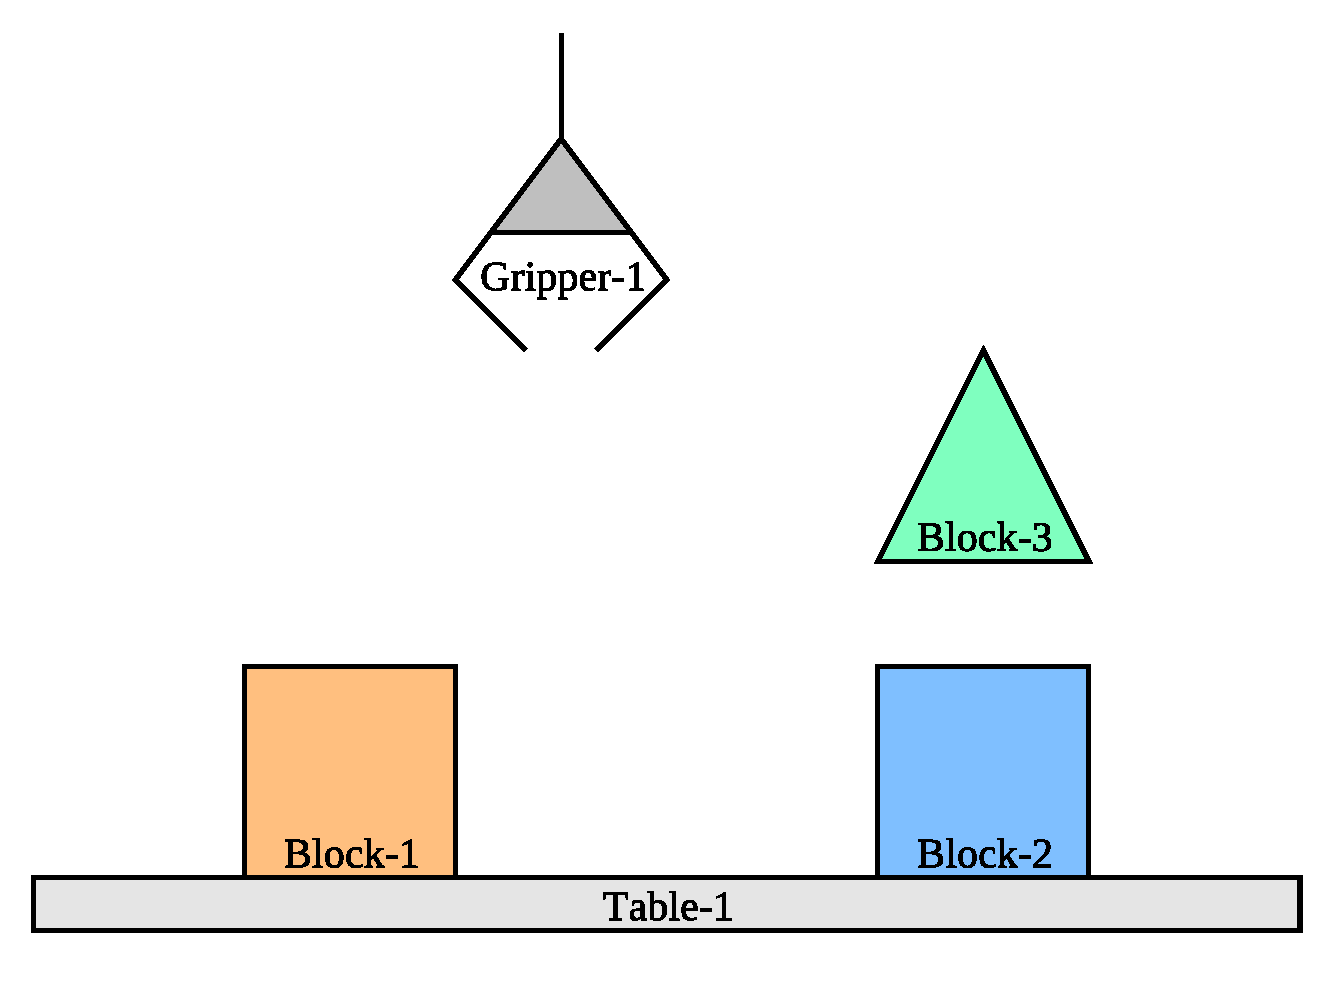
\includegraphics[width=11cm]{gfx/blocks_world_screenshot-1}
  \caption[Blocks world is a simple real-time symbolic control problem.]{Blocks world is a simple real-time symbolic control problem that I use to demonstrate my reflective control learning theory.}
  \label{fig:blocks_world_screenshot-1}
\end{figure}

I use blocks world, a canonical toy AI problem, in order to demonstrate my example of reflectively learning to plan.
See Figure~\ref{fig:blocks_world_screenshot-1} for a screenshot of my blocks world problem physical simulation.

\begin{table}
  \myfloatalign
  \begin{tabularx}{\textwidth}{XllX}
    & [Gripper-1 is me] & [Gripper-1 movement\_command []] & \\
    & [Gripper-1 is-a gripper] & [Gripper-1 color black] & \\
    & [Gripper-1 is-holding []] & [Block-1 is-a block] & \\
    & [Block-1 color brown] & [Block-1 shape cube] & \\
    & [Block-1 on Table-1] & [Block-1 left-of Gripper-1] & \\
    & [Block-2 is-a block] & [Block-2 color blue] & \\
    & [Block-2 shape cube] & [Block-2 on Table-1] & \\
    & [Block-2 right-of Gripper-1] & [Block-3 is-a block] & \\
    & [Block-3 color green] & [Block-3 shape pyramid] & \\
    & [Block-3 right-of Gripper-1] & [Table-1 is-a block] & \\
    & [Table-1 color white] & [Table-1 shape cube] & \\
    & [Table-1 left-of Gripper-1] & &
  \end{tabularx}
  \caption[Blocks world agent perceptual input.]{Blocks world agent perceptual input.}
  \label{tab:blocks_world_agent_perceptions}
\end{table}

See Table~\ref{tab:blocks_world_agent_perceptions} for an example set of perceptual input that corresponds with the physical situation shown in Figure~\ref{fig:blocks_world_screenshot-1}.

\section{Working in a World of Building Blocks}

In his PhD thesis, Terry Winograd worked in the world of building
blocks \citep{winograd:1970}.  This program maintained traces of its
goals and subgoals, which enabled it to answer questions about why it
performed certain actions.  This system worked because it stored
goals.

Knowing the goal state of the computation is important, and I do not
ignore this aspect in tracing the deliberative layer.  My system is
able to answer these sorts of questions, as this simply requires
climbing the stack of mental resource activations, but when debugging
the deliberative process, it is helpful to not only know the ending
point of computation but also the means toward that end.

\section{Terry Winograd's SHRDLU and Goal Tracing}

I am building upon what was learned from Winograd's thesis
\citep{winograd:1970} in terms of using traces of the deliberative
process as well as using a semantic model of the world in order to
understand communications between agents.  I have chosen to use a
simpler and more direct language interface between agents that refers
more directly to the semantic information and mental processes
involved.  I have experimented with implementing the original SHRDLU
english language parser, although I believe the parsing process can be
better controlled as a goal-oriented set of concurrent processes than
as the stack-based depth first search that I started writing in my
initial experiments.

\section{Why Not Work Within a Building Blocks Domain?}

The building blocks approach is a good precedent.  However, there are
many problems with only demonstrating a solution on a toy problem.
First, an approach demonstrated to solve a small problem, often do not
scale to larger problem domains of similar complexity.  So, I feel
that it is important to show the same reflective approach to learning
can also be applied to a domain with a much larger state space than
the toy blocks world problem.  I then, have shown the theoretical
gains of my approach by using the canonical model as a tool for
explanation, and now I show that my model does scale to larger
problem domains of only slightly more complexity.  See
\cite{smith:2010} for a discussion of the benefits of approaching the
social commonsense reasoning problem with a physical simulation of a
kitchen.

I have conscripted my domain of object types in the kitchen, such
that it is currently comparable to the number of object types that
Winograd used in his thesis.  My object types do have different ways
that they may be used, which is a small addition of complexity.
Although I do not introduce many of the complexities of ontological
reasoning, a common approach to commonsense reasoning, e.g. Cyc
\citep{lenat:1990}, my system demonstrates an important new approach
to commonsense reasoning that grounds learning by being told in the
domain of goal-oriented reasoning, which allows organizing and
debugging knowledge in terms of what goals it is useful for
accomplishing.

\section{A Physical Simulation of a Kitchen as a Social Commonsense Reasoning Domain}

\begin{figure}[bth]
  \center
  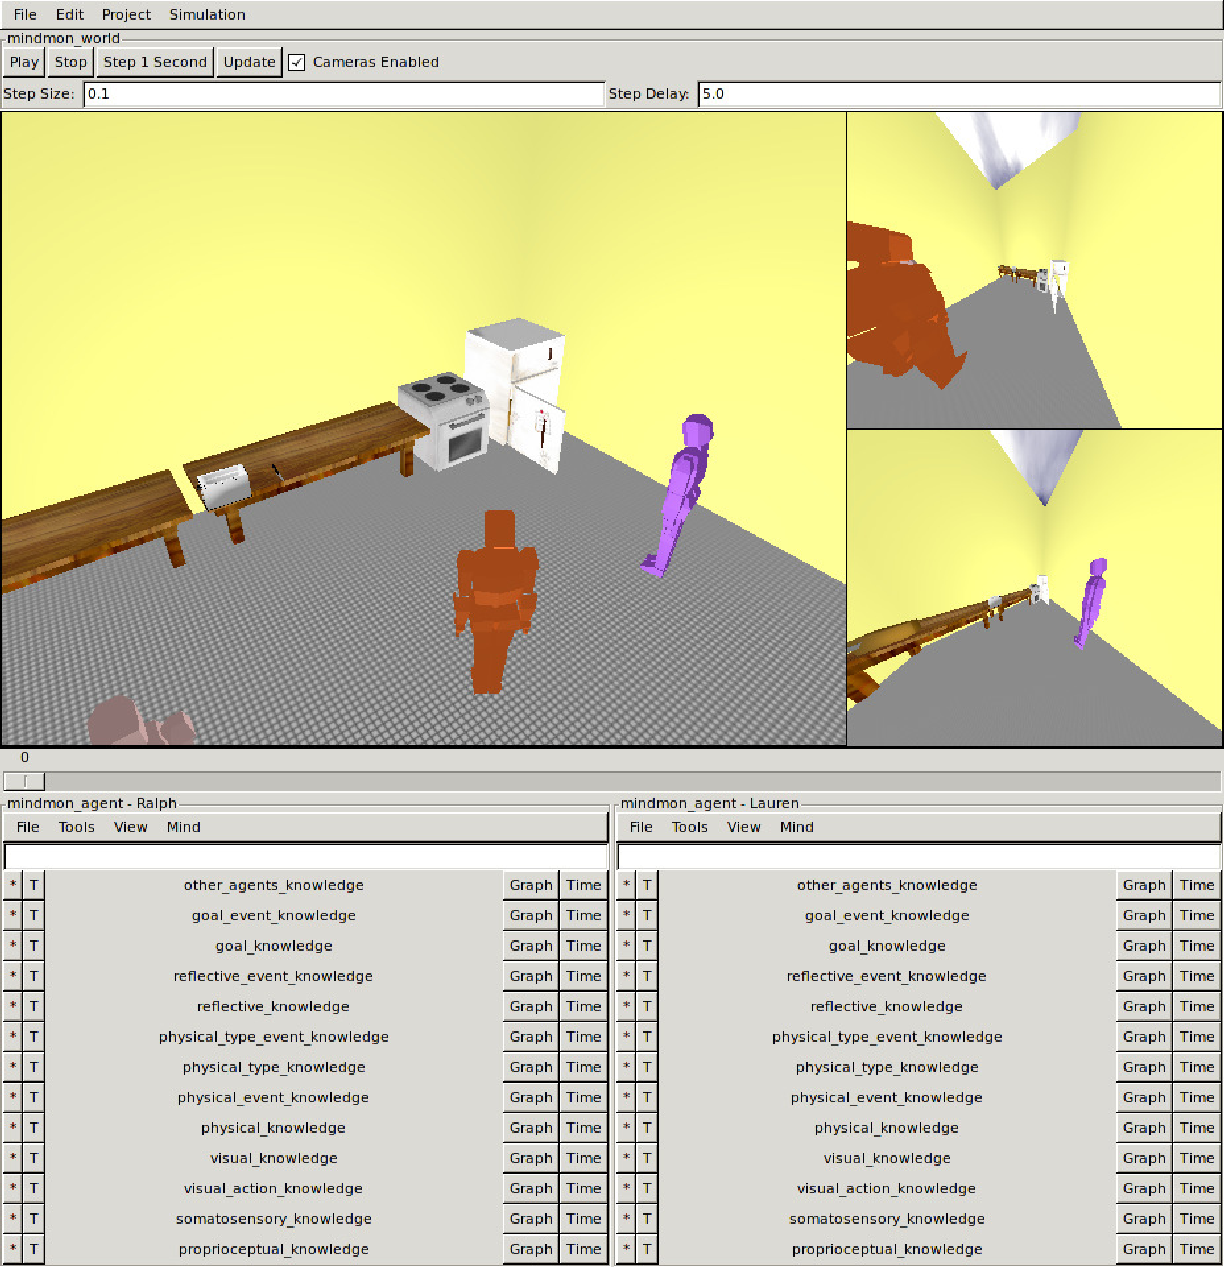
\includegraphics[width=11cm]{gfx/mindmon-isis_world-screenshot-1}
  \caption[Isis World is a larger physical simulation than the Blocks
    World toy problem.]{Isis World is a larger real-time symbolic
    physical simulation, which I use to demonstrate that my reflective
    goal-oriented learning approach scales to the physical and
    reflective problem spaces of slightly more complicated learning
    problems.}
  \label{fig:mindmon-isis_world-screenshot-1}
\end{figure}

I have experimented with applying my cognitive architecture to a
larger social commonsense reasoning domain with parents that teach
children as they attempt to accomplish cooking tasks in a kitchen.
See \cite{morgan:2011} for details about my six-layered reflective
theory of social and moral reasoning, which assumes the existence of a
procedurally reflective infrastructure with a reflective problem
solver written within it.  From an educational perspective,
\cite{dewey:1907} has theorized that kitchens are a good example of a
rich learning environment for children.  Some form of kitchen, or a
social place where food is cooked for a family, is ubiquitous across
cultures.  Kitchens have a clear production goal, namely food.  Many
mental realms must be used in accomplishing even simple cooking goals,
including: math, physics, chemistry, thermodynamics, language,
society, family, imprimer learning, concurrent planning, etc.  See
Figure~\ref{fig:mindmon-isis_world-screenshot-1} for a screenshot of
my graphical user interface to the cognitive architecture, while it
interacts with the Isis World physical simulation.


\cleardoublepage\part{Conclusion}\label{part:conclusion}
%%*****************************************
\chapter{Results}\label{ch:results}
%*****************************************


\section{Reflective Knowledge Substrate}


\subsection{General Parallelism and Concurrency}

My system is built to handle concurrent parallel processes on
multi-core operating systems.  In this section, I test how efficient
my implementation of concurrency performs on a number of standard
concurrency timing tasks.  In an ideal situation, given $N$ processor
core working on independenct problems, I should get a factor of $N$
speedup.  Because multiple core processors share memory resources this
ideal is never actualized, so we test our implementations performance
by developing appropriate metrics.

\subsection{Program as Data}

In systems where the program is data, a bottleneck in writing programs
that write programs is the efficiency of the run-time compiler.  In
this section we test the relative performance of our compiler in
our-time system.

\section{Layered Reflective Problem Solving}

In this section, I evaluate how well different configurations of my
learning system accomplishes a range of goals in the blocks world
environment.

\subsection{Comparison between Learned Reactions and Planning}

I evaluate how adding or removing reflectively learning to plan
changes the performance of the blocks world goal accomplishment
metric.

\subsection{Analogy between Physical Goals and Planning Goals}

I evaluate how adding or removing the second layer of reflectively
learning to plan changes the performance of the blocks world goal
accomplishment metric.

\section{Learning by Credit Assignment}

\subsection{Tracing Knowledge Provenance for Credit Assignment of Success or Failure}

I evaluate how tracing causality of knowledge provenance can improve
learning performance according to the blocks world goal accomplishment
metric.


%************************************************
\chapter{Evaluation}
\label{chapter:evaluation}
%************************************************

This dissertation consists of four contributions that work together to
form the SALS AI.  From the low-level virtual machine and Lisp-like
programming language to the reflective and super-reflective layers of
the Emotion Machine cognitive architecture, it is difficult to
evaluate all aspects of the SALS AI by a single simple metric.
Therefore, this chapter presents a number of different metrics that
are used to measure all of the four contributions presented in this
dissertation:
\begin{packed_enumerate}
\item{\emph{Emotion Machine Cognitive Architecture}: The primary
  contribution of this thesis is a recursive implementation of a
  reflective planning layer that controls a deliberative planning
  process.  Because of the recursive nature of the implementation, a
  super-reflective layer is also used to control and learn about the
  reflective planning process.  The benefit of adding each additional
  reflective layer is that more can be learned from each deliberative
  failure by adding each additional reflective layer, but there is a
  computational trade-off in that each additional reflective layer
  also increases the computational complexity of the overall
  architecture.  This chapter evaluates the Emotion Machine cognitive
  architectural component of the SALS AI by asking the following
  question: What is the increase in computational complexity
  introduced by adding additional reflective planning layers to the
  basic deliberative planning process?  The answer to this question is
  not at first obvious because of the exponentially larger state-space
  confronted by each higher planning layer.  The result is that each
  additional layer adds a roughly linear increase in computational
  complexity to the overall architecture.  This chapter discusses how
  the increased computational complexity of each additional reflective
  planning layer is kept from becoming exponential in the SALS AI.
  This chapter also discusses how using concurrent hardware in order
  to separately simulate each additional reflective layer has the
  potential to reduce the overall time-complexity of the architecture
  to sub-linear per additional layer.}
\item{\emph{Learning from Being Told Natural Language Plans}: The
  ability of each planning layer in the SALS AI to interpret and
  imagine the effects of ambiguous natural language plans relies on a
  search through possible interpretations of each natural language
  phrase in any given plan.  This search would quickly become
  intractable if it were not controlled by a number of different types
  of low-level programmatic constraints.  Only those natural language
  plan interpretations that make programmatic sense according to these
  constraints are further considered for imagination or execution.  In
  practice, each low-level constraint helps to reduce the overall
  search complexity by varying amounts depending on the domain of
  control, whether the natural language plan is describing a control
  process for the physical, deliberative, or reflective knowledge
  domains.  This chapter shows empirical results that compare the size
  of the overall natural language plan interpretation search with and
  without each of these constraints for the control of each knowledge
  domain in the SALS AI.  This chapter also discusses the trade-offs
  between introducing language specific constraints, such as
  English-only semantics or syntax, versus purely programmatic
  constraints that keep the SALS natural planning language as it is
  currently applicable to all natural human languages.}
\item{\emph{Learning Asynchronously from Experience}: The ability of
  each planning layer in the SALS AI to asynchronously abstract the
  partial state events in its control knowledge domain as well as
  asynchronously learn rule-based causal models of resource
  activations of the layer below introduces two potentially
  problematic scaling factors for the computational complexity of the
  overall SALS AI.  Firstly, the number of partial states in arbitrary
  knowledge domains could in the worst case introduce a factorial
  growth with the size of the knowledge domain and the size of the
  partial states being abstracted.  As factorial growth would be an
  intractable scaling factor for the computational complexity, this
  chapter shows empirical evidence for the actual scaling factors for
  abstracting partial states from each of the control knowledge
  domains, including the physical, deliberative, and reflective
  knowledge domains.  The causal hypothesis rule-learning algorithm
  could potentially even have a worse scaling factor that is a
  multiplier on the number of partial states abstracted in the first
  asynchronous stage in the SALS AI's learning from experience.  This
  chapter will also present empirical evidence of the actual scaling
  factor introduced by the conjunctive rule-learning algorithm
  employed in learning causal models of resource activations in the
  SALS AI for each planning layer, including the deliberative,
  reflective, and super-reflective layers.}
\item{\emph{Virtual Machine and Programming Language}: The SALS AI is
  constructed on a low-level virtual machine and Lisp-like programming
  language that takes advantage of multithreaded and multicore CPUs.
  The SALS virtual machine executes concurrent bytecode processes that
  are called ``fibers,'' which are an abstraction of the POSIX threads
  provided by the underlying operating system.  In order to minimize
  hyperthread-specific cache-miss effects for each concurrently
  executing fiber, a separate memory pool is allocated for each
  hardware hyperthread in each CPU core in the underlying hardware
  platform.  The SALS virtual machine performs dynamic load balancing
  in order to take advantage of as many CPU cores as possible while
  executing multiple fibers.  Also, the SALS virtual machine includes
  a concurrent tricolor garbage collection algorithm that has been
  optimized to be used over multiple memory pools.  In a perfect
  symmetric multiprocessing (SMP) system, executing $N$ fibers on $N$
  processors should have a constant time-complexity, but modern
  multithreaded and multicore CPUs have shared caches between
  hyperthreads and cores, which makes systems based on these CPUs less
  than ideal SMPs.  Furthermore, mutual exclusion (mutex) locks
  required for garbage collection slow down garbage collection across
  multiple memory pools by a factor depending on the number of
  cross-references between pools.  This chapter empirically evaluates
  how the SALS virtual machine performs at minimizing these cache-miss
  and locking effects on an Intel Core i7 CPU, which has 4 cores, each
  with 2 hyperthreads, while executing various numbers of concurrent
  fibers.}
\end{packed_enumerate}

\section{Computational Complexity of Reflective Layers}

The SALS AI consists of 100 parallel heterogeneous resources,
organized into 29 agencies, which comprise the 5 layers.  The causal
procedurally reflective tracing features of the SALS virtual machine
that have been described in
{\mbox{\autoref{chapter:virtual_machine_and_programming_language}}}
allow for the run-time evaluation of each separate causally scoped
component of the SALS AI.  In the evaluation of the complexity of each
additional reflective layer, the following execution events are
measured:
\begin{packed_enumerate}
\item{Memory Allocation in Bytes}
\item{Garbage Collection in Bytes}
\item{Bytecode Execution Count}
\item{Semantic Frame Slot Mutations}
\item{Plan Interpretation Nodes Considered}
\item{Analogical Plan Matches Considered}
\end{packed_enumerate}
Each planning layer in the SALS AI can be used to specify very similar
types of goals.  For example, consider the following three different
pieces of knowledge:
\begin{packed_enumerate}
\item{``A pyramid is on a cube.''}
\item{``A deliberative planner has the positive goal for a pyramid to
  be on a cube.''}
\item{``A reflective planner has the positive goal for a deliberative
  planner to have the positive goal for a pyramid to be on a cube.''}
\end{packed_enumerate}
This is the feared, worst-case scenario that the analogical language
interpretation process in each subsequently higher reflective layer of
reasoning becomes an exponentially more difficult problem.  In
general, however, this is not true because reflective reasoning does
not and in practice often does not involve directly interpreting these
types of exponentially more difficult natural language interpretation
problems.  This is because reflective natural language plans are very
rarely directly about specific states of knowledge in the physical
knowledge base as in these examples.  Usually, reflective knowledge is
about much simpler partial states of the deliberative planning machine
that do not involve any physical knowledge at all.  For example,
consider the following pieces of knowledge:
\begin{packed_enumerate}
\item{``A deliberative planner is focused on a plan that has failed.''}
\item{``A reflective planner is focused on a plan that has failed.''}
\end{packed_enumerate}

{\mbox{\autoref{table:plan_interpretation_computational_complexity_of_layers}}}
shows measures of computational complexity for each planning layer in
SALS AI as it goes through the learning scenario presented in the
introduction to this dissertation.
\begin{table}
\centering
\begin{tabular}{|l|l|l|l|l|}
\hline
                 &Alloc &GC &BC &Mutate \\
\hline
Deliberative     &      &   &   &       \\
\hline
Reflective       &      &   &   &       \\
\hline
Super Reflective &      &   &   &       \\
\hline
\end{tabular}
\caption{Computational complexity of plan interpretation for each
  planning layer.}
\label{table:plan_interpretation_computational_complexity_of_layers}
\end{table}
In order to measure the increase in computational complexity
introduced by adding additional reflective planning layers to the
basic deliberative planning process,   While more can be learned from
each deliberative failure by adding additional reflective planning
layers, each additional reflective layer also increases the
computational complexity of the overall architecture.  First, let us
consider the computational complexity of the deliberative planning
layer.

The answer to this question is not at first obvious because of the
exponentially larger state-space confronted by each higher planning
layer.

The result is that each additional layer adds a roughly linear
increase in computational complexity to the overall architecture.

This chapter discusses how the increased computational complexity of
each additional reflective planning layer is kept from becoming
exponential in the SALS AI.

This chapter also discusses how using concurrent hardware in order to
separately simulate each additional reflective layer has the potential
to reduce the overall time-complexity of the architecture to
sub-linear per additional layer.

\section{Computational Scaling of Natural Language Interpretation Constraints}

\section{Computational Scaling of Partial State Abstraction and Rule-Learning}

Given that each planning layer in the SALS AI is based on perceiving
and acting based on the existence or non-existence of partial states
in the knowledge base that is being controlled by the planning layer,
the state-space of the control domain that is perceived and reacted to
by a planning layer is directly related to the number of partial
states that can be abstracted from this control domain.  For example,
if we consider that the knowledge base that is being controlled by a
given planning layer is represented as a graph, which is not exactly
correct but will suit our purposes here, the set of partial states
that can be abstracted from this control domain includes a subset of
all possible subgraphs of this graph representation.  In order to
avoid an intractable number of partial states being automatically
abstracted from a given knowledge base, the types of partial states
that the SALS AI abstracts are limited to the ``relationship'' and
``property'' types of partial states described in
{\mbox{\autoref{chapter:learning_asynchronously_from_experience}}}.
These simple types of partial states limit the complexity



%\begin{equation}
%({2^n}-1)\left(\frac{n(n-1)}{2}\right)^{\ell}
%\end{equation}


\section{Computational Scaling of Concurrent Processing Hardware}


%% \section{old stuff}

%% \section{Boot-up and Perceive Experiment}

%% As an initial evaluation of the run-time performance of the AI, I have
%% run an experiment that simply initializes the AI and lets it perceive
%% the world over time.  The physical world does not change during this
%% experiment and the AI is not given any goals to accomplish, so this
%% experiment is a control that shows the baseline memory usage and
%% run-time performance of the cognitive architecture in its ``idling''
%% mode.  This experiment shows that the mind takes $10$ minutes to
%% initialize.  After initializing, the AI learns from its initial
%% perception and continues to attempt to detect changes in its raw
%% visual input over the next $50$ minutes.  Over the $50$ minutes of
%% continuous perception, the mind uses a highly fluctuating amount of
%% memory that stays, on average, relatively constant.  The mind is not
%% static in this experiment.  The mind contains resources that allocate
%% an average of $1.8$ megabytes per second in the built-in reactive
%% layer process of detecting visual changes in the next state from the
%% physical simulation, so that these changes may be propagated to the
%% physical knowledge of the learned reactive layer in a stream of
%% events.  Over $6$ gigabytes of memory is allocated over the entire
%% $60$ minutes of the experiment.  The mind uses an average memory
%% footprint of about $26$ megabytes over the course of the experiment.
%% The bytecode execution rate stabilizes at about $12$ thousand
%% bytecodes per second.  The concurrent processing capabilities of the
%% architecture can handle bursts of $50$ thousand bytecodes per second,
%% but this experiment simply shows that the execution rate of the
%% architecture does not slow down over time.  The entire cognitive
%% architecture exhibits stable handling of continuous processing for
%% experiments lasting over an hour, handling the allocation and garbage
%% collection of many gigabytes of memory in the process.
%% {\mbox{\autoref{figure:data/bootup_evaluation/mind_plot-Gripper-1}}}
%% shows a plotted overview of the run-time performance of the AI during
%% the boot-up and perceive experiment.  \autoref{table:bootup} on page
%% \pageref{table:bootup} shows more detailed plots for the run-time
%% behavior of each individual layer and agency within the AI.
%% %\experimentAIdatafigures[60]{bootup_evaluation}{an experiment that
%% %  boots up the AI, allowing it to continue to perceive the physical
%% %  world over time without stimulating it to achieve any goals.  This
%% %  experiment shows that the AI learns from its initial perceptions,
%% %  and when these do not change, it has nothing to learn and memory
%% %  usage is stable.}

%% \section{Deliberative Learning Experiment without Reflection}

%% The second run-time experiment that was performed with the cognitive
%% architecture does not include the reflective learning component that
%% learns hypothetical models for how the deliberative resources modify
%% the planning machine type knowledge base.  The AI is initialized,
%% which takes the same $10$ minutes as in the initial experiment.  The
%% AI is then told to execute a deliberative plan, which causes it to
%% execute a plan that attempts to stack a cube on top of a pyramid.  In
%% learning the effects of reactive resource executions on the physical
%% type knowledge bases the deliberative AI allocates $5.3$ megabytes per
%% second, while the memory footprint only grows at a rate of $90$
%% thousand bytes per second due to the learning that occurs over the
%% $60$ minutes that it takes to fail to accomplish this goal.  The AI
%% does not respond to the failure because the reflective layers are not
%% active.  The AI allocates an average of $1.2$ megabytes of memory per
%% second for the length of the experiment, which results in a total of
%% $5.4$ gigabytes over the course of the experiment.  The architecture
%% executes an average of $11$ thousand bytecodes per second over the
%% course of the experiment.  This shows that the architecture slows down
%% when more resources are active than simply the reactive perceptual
%% resources.  As deliberative learning resources become active, the
%% bytecode rate does not decrease much from the $12$ thousand bytecodes
%% per second in the control, but the overall memory allocation rate does
%% decrease by a factor of $66$\% from $1.8$ megabytes per second in the
%% control to $1.2$ megabytes per second with deliberative learning
%% enabled.
%% {\mbox{\autoref{figure:data/no_reflective_learning_evaluation/mind_plot-Gripper-1}}}
%% shows a plotted overview of the run-time performance of the AI during
%% the deliberative learning experiment with the reflective layer
%% disabled.  \autoref{table:no_reflective_learning} on page
%% \pageref{table:no_reflective_learning} shows plots of data for the
%% entire mind, each layer, as well as each agency within each layer for
%% this deliberative learning experiment.
%% %\experimentAIdatafigures[75]{no_reflective_learning_evaluation}{an
%% %  experiment with the reflective tracing of the deliberative process
%% %  disabled.  This experiment can be compared with run-time behavior of
%% %  the full AI cognitive architecture, which can learn from the failure
%% %  and initiate a second attempt at plan selection and execution.}

%% \section{Deliberative and Reflective Learning Experiment (The Full Architecture)}

%% The third run-time experiment that was performed with the cognitive
%% architecture includes both the deliberative as well as reflective
%% learning layers.  The deliberative layer learns hypothetical models of
%% the reactive resource execution effects on the physical type knowledge
%% base, while the reflective layer learns hypothetical models of the
%% deliberative resource execution effects on the deliberative planning
%% machine type knowledge base.  Although this experiment involves an
%% initial imaginative and plan selection processes in the reflective
%% layer, this experiment runs very similarly through the first $75$
%% minutes of otherwise mostly deliberative and reactive resource
%% executions.  Around minute $75$, the cognitive architecture responds
%% to the failure in the deliberative planning machine with the
%% reflective bug response, which begins another round of reflective
%% learning, imagination, and refined plan selection.  After a reflective
%% bug response, the goal is accomplished successfully around minute
%% $105$.  The experiment is allowed to run continuously after this point
%% for a total of $180$ minutes in order to show the performance of
%% baseline perceptual activity after going through the complete process
%% of deliberative and reflective learning.  Except for a blip at minute
%% $135$, which requires an extended garbage collection period, the AI is
%% otherwise stable after both layers have successfully demonstrated
%% learning.  With the addition of the reflective learning layer in the
%% final experiment the average bytecode execution rate has dropped
%% significantly, running at a factor $55$\% of the execution rate of the
%% architecture in the experiment demonstrating only deliberative
%% learning.  This experiment demonstrates the taxing demand of the extra
%% concurrent processes and memory allocation required with the
%% additional reflective learning algorithm.  However, slowing the
%% algorithm down by a factor of two with the addition of a reflective
%% layer of learning shows that the slow down is roughly linear with the
%% additional layer.  For example, in a naive approach to reflective
%% learning, an exponential increase in processing would be expected
%% because all resource executions and knowledge in the layers below
%% would be reflected upon and modelled by the reflective layer.  Because
%% the reflective learner implemented in this architecture only reflects
%% over the deliberative planning machine and not all of the processing
%% in the layers below, this architecture shows a linear slowdown with
%% the addition of reflective layers of learning.
%% {\mbox{\autoref{figure:data/reflective_learning_evaluation/mind_plot-Gripper-1}}}
%% shows a plotted overview of the run-time performance of the AI during
%% the reflective learning experiment.
%% \autoref{table:reflective_learning} on page
%% \pageref{table:reflective_learning} shows plots of data for the entire
%% mind, each layer, as well as each agency within each layer for this
%% reflective learning experiment, showing the run-time performance of
%% the full architecture.
%% %\experimentAIdatafigures[180]{reflective_learning_evaluation}{an
%% %  experiment testing the full AI cognitive architecture, including the
%% %  reflective tracing of the deliberative planning process, imagining
%% %  the potential failures of the deliberative planning machine as well
%% %  as the physical effects of physical actions.}

%% \section{No Theoretical Slowdown of Original Algorithm}

%% In order to assume that there is no theoretical slowdown of the
%% original planning algorithm when reflective learning is applied, it
%% must be assumed that the reflective implementation is an ideal
%% concurrent shared memory architecture.  In practice, the underlying
%% Funk virtual operating system slows down when more concurrent and
%% parallel tasks are executing.  This is beside the theoretical point,
%% but the following table shows a real-time test of the actual slowdown
%% experienced by the Funk operating system as different numbers of
%% parallel tasks are executed to perform a simple numerical processing
%% task.  The test was done on a dual Pentium processor computer, each
%% with ``core duo'' technology with each core implementing
%% ``hyper-threading'', which ends up appearing as eight processors to
%% the Linux operating system underlying the Funk virtual operating
%% system:

%% \vspace{5mm}
%% \begin{tabular}{ll}
%% Tasks & Real-Time (s) \\
%% 1 & 29\\
%% 2 & 36\\
%% 3 & 46\\
%% 4 & 44\\
%% 5 & 68\\
%% 6 & 67\\
%% 7 & 73\\
%% 8 & 110\\
%% \end{tabular}
%% \vspace{5mm}

%% As each additional concurrent resource in the cognitive architecture
%% begins execution, this table shows the approximate slowdown that the
%% Funk virtual machine experiences on this specific dual processor
%% hardware.


%*****************************************
\chapter{Future}\label{chapter:future}
%*****************************************

\label{section:model_6_future_research}

I began discussing strong parallels between my model and Minsky's
six-layered reflective theory of mind, called The Emotion Machine or
Model-6, in \autoref{backreference:self_reflective_self_conscious}.
Now I will continue a description of the top two layers of Minsky's
model in the theoretical terms of my model.

\section{Objective Reflection}

The ability to abstract object and subject distinctions within the
mind is key to how I see the creation of selves.  The primary object
abstractions would necessarily be based on physical activities that
lead toward or against physical goals.  An object has subjective
perspectives and extents in Space.  Further, every subjective
perspective would usefully have a set of causal hypotheses that lead
to and away from the object's more central subjective perspectives.
Objects, therefore, become collections of subjective perspectives that
can be easily traversed given the included causal models.  The extent
of an object in Space gives a useful Spatial arrangement for causal
hypotheses that help to create controllable boundaries around similar
perceptual and goal activities.

For example, this makes sense from a survivability standpoint.  The
most important and the first subject and object distinctions are those
that help accomplish or avoid physical goals.  In creating the
distinction that allows the mind to see the physical body as subjected
to the objects of a physical world, the mind has created one of the
first subjective perspectives, the physical body.

\section{Circular Objects}

Causal hypotheses are used in order to predict the future occurrence
of symbolic perceptions and goals.  Through reflective thinking, plans
are constructed from causal hypotheses consistent with the past,
elaborating the necessities in the past and the results in the future.
Analogies between consistent plans can be abstracted into models of
objects.  For example, a plan that begins and ends with the same
symbolic perception could be considered an example of a ``circular''
object; thus, an analogical plan abstraction would represent a type of
object, that has multiple sides to perceive depending on the subject's
position in the plan.  Circular objects may be an important type of
object to analogically recognize because a circular object allows one
to perform actions while being able to get back to a known perceptual
symbol.  If one is in a known circular object, then one is not lost in
the sense that one can always follow the circle in order to get back
to any perceptual symbol contained within the circular plan object.
My implementation includes tools for performing analogical
abstractions and constructions of plans, but this machinery is not key
to my thesis of explaining causal reflective learning to accomplish
goals.  I include this section in the dissertation to eliminate a
potential confusion that would conflate the concept of symbol with
that of object.  Symbols are the most primitive elements available to
thinking, while objects are more complicated in that they are composed
of analogical consistencies between plans that are themselves composed
of many symbols.  Objects have multiple subjective perspectives.
Objects are artificial creations of a mind, based on artificial static
symbols representing the ongoing activity in Duration.

\section{Body and World}

An intelligent mind builds models that predict the occurrence of
perceptual symbols.  Analogical thinking is used to abstract objects
and simultaneously the implied subjective perspectives on these
objects as they are manipulated.  The separation between the physical
body and the physical world is an objective form of thinking that is
fundamentally caused by goals that emphasize distinguishing bodily and
worldly goals in the causal structures of the physical perceptions.
For example, physical actions that change physical perceptions in
predictable ways are often bodily physical perceptions, i.e. moving
ones hand in front of ones face causes one to consistently see a hand.
Also, physical pain perceptions could be related to physical goals
that emphasize the artificial separation between the body and the
world.  Understanding the artificial separation of the body and the
world allows for an objective form of scientific study that places the
object of study in the world outside of the effects of the body.

\section{$m^\text{th}$-Stratum Objective Reflection}

Above this ability to model multiple interacting objects is the
ability to model objects as containing objects of the self-same type.
The ability to abstract all of the layers of a reflective mind into
one type of object or another can be used to recursively model one
object's model of another object.  Therefore, although my model does
not include objective reflection, I see this form of reflection as
along a new dimension that has, as its origin, all of the reflective
layers that I have so far described in my model.  I will refer to this
new dimension as ordered \emph{strata} of the \emph{objective
  dimension of reflective thinking}.

\begin{align}
\label{equation:objective_0_reflective_stratum}
\text{objective}^0\text{ reflective stratum } &{\approx} \bigcup_{n=0}^{\infty}{\text{reflective}^n\text{ layer}} \\
\label{equation:objective_m_reflective_stratum}
\text{objective}^m\text{ reflective stratum } &{\approx} \bigcup_{n=0}^{\infty}{\text{objective}^m\text{ reflective}^n\text{ layer}}
\end{align}

Prior to the first objective thinking stratum existing, it must have a
prior part of the mind upon which to objectively reflect.  I will
refer to all of the reflective layers I've described so far as the
zeroth-stratum of objective thinking, the ``$\text{objective}^0$''
stratum, since it contains no objective thinking at all.  Therefore,
the $m^\text{th}$-stratum of objective thinking in my model can be
described as ``$\text{objective}^m$'' reflective thinking.  Given this
notation, the self-reflective layer of Minsky's model would be the
first-stratum of objective thinking, or $\text{objective}^1$ reflection,
in my model.  Each $\text{objective}^m$ reflective stratum in my model
contains an infinite number of $\text{objective}^m\text{ reflective}^n$
layers.
Equations~\ref{equation:objective_0_reflective_stratum}~and~\ref{equation:objective_m_reflective_stratum},
roughly and non-mathematically show how each objective thinking
stratum is composed of an infinite number of reflective layers.
Again, this notation is \emph{not} set theoretic, and thus, set
theoretical mathematics do not apply.

\begin{figure}[bth]
  \begin{align*}
    \left.
    \begin{array}{l}
      \text{Minsky's Problem Domain }\\
      \text{Minsky's Built-in Reactive Layer }\\
      \text{Minsky's Learned Reactive Layer }\\
      \text{Minsky's Deliberative Layer }\\
      \text{Minsky's Reflective Layer }\\
    \end{array}
    \right\}                               &{\approx} \bigcup_{n=0}^{\infty}{\text{objective}^0\text{ reflective}^n\text{ layer}} \\
                                           &{\approx} \text{ objective}^0\text{ reflective stratum} \\
  \end{align*}
  \begin{align*}
    \text{Minsky's Self-Reflective Layer } &{\approx} \bigcup_{n=0}^{\infty}{\text{objective}^1\text{ reflective}^n\text{ layer}} \\
                                           &{\approx} \text{ objective}^1\text{ reflective stratum} \\
  \end{align*}
  \begin{align*}
    \text{Minsky's Self-Conscious Layer }  &{\approx} \bigcup_{n=0}^{\infty}{\text{objective}^2\text{ reflective}^n\text{ layer}} \\
                                           &{\approx} \text{ objective}^2\text{ reflective stratum}
  \end{align*}
\caption{The top layers of Model-6 roughly mapped to my
  $\text{objective}^m\text{ reflective}^n$ stratum notation.}
\label{figure:model_6_as_reflective_stratum_notation}
\end{figure}

Minsky's ``self-conscious'' layer would thereby roughly correspond
with my $\text{objective}^2$ reflective stratum.  Having two levels of
recursion in a objective thinking sense, leads to the ability to
represent what one object references in terms of what another object
references in terms of the original object.
\autoref{figure:model_6_as_reflective_stratum_notation} shows roughly
how the levels of Minsky's theory can be related to my stratum
notation.

\section{Imprimers}

\cite{minsky:2006} explains that terms like ``guilt'' and ``pride''
can refer to self-conscious ways of thinking.  Minsky hypothesizes
that there are powerful ways of thinking that result when someone whom
one respects, like a parent, values or devalues their goals.  This
type of relationship between object models is named an \emph{imprimer
  relationship} by Minsky.  In this relationship, the parent plays the
role of what Minsky has named an \emph{imprimer}, in reference to the
ability of ducklings to learn, relatively arbitrarily, to trust and
follow a parent-like figure.  Since I do not know of a another word
for an object in this sort of imprinting relationship, I will simply
use Minsky's term: imprimer.  He hypothesizes that imprimers, such as
parents and caregivers, play an important role in unquestioned
knowledge inheritance in children.  This type of thinking about what
someone else is thinking about their goals requires at least two
strata of objective reflection in my model.



% 1. models of cognition intro
% 2. literature of cognition/ commonsense (s)
% 3. problems i will solve
% 4. theory and alternatives
% 5. a system
% 6. experiments with it
% 7. discussion (how it can integrate and expand on and changes what will happen
% 8. future


%*******************************************************
% Backmatter
%*******************************************************
\appendix
\cleardoublepage\part{Appendix}
%************************************************
\chapter{Science}
\label{chapter:science}
%************************************************

Physically objectifying problems scientifically has proved useful.
The primary utility of this understanding is that the scientist can be
replaced by another scientist and the experimental results can be
duplicated.  Arbitrary replacement of the subjective scientist implies
the potential for mechanical simulation of the physical phenomenon,
reducing the subjective scientist to a purely perceptual role.
Mechanical duplication of human labor leads to increased efficiency
and productivity.  First, steam engines were a model of autonomous
human activity.  Next, computers became the physical model of choice.
Now, various humanoid robots have included electrical motors and
computers to become closer reproductions of human physical abilities.
Thus, understanding a model of mind has become important in
duplicating more complex human physical behaviors that require
thinking.  The mechanical duplication of human thinking is the goal of
the field of AI.  Only the simplest forms of human thinking have been
coherently mechanized thus far.

\section{Object and Subject}

Causal hypotheses are used in order to predict the future occurrence
of symbolic perceptions and goals.  Through reflective thinking, plans
are constructed from causal hypotheses consistent with the past,
elaborating the necessities in the past and the results in the future.
Analogies between consistent plans can be abstracted into models of
objects.  For example, a plan that begins and ends with the same
symbolic perception could be considered an example of a ``circular''
object; thus, an analogical plan abstraction would represent a type of
object, that has multiple sides to perceive depending on the subject's
position in the plan.  Circular objects may be an important type of
object to analogically recognize because a circular object allows one
to perform actions while being able to get back to a known perceptual
symbol.  If one is in a known circular object, then one is not lost in
the sense that one can always follow the circle in order to get back
to any perceptual symbol contained within the circular plan object.
My implementation includes tools for performing analogical
abstractions and constructions of plans, but this machinery is not key
to my thesis of explaining causal reflective learning to accomplish
goals.  I include this section in the dissertation to eliminate a
potential confusion that would conflate the concept of symbol with
that of object.  Symbols are the most primitive elements available to
thinking, while objects are more complicated in that they are composed
of analogical consistencies between plans that are themselves composed
of many symbols.  Objects have multiple subjective perspectives.
Objects are static creations of a mind, based on static symbols
representing the ongoing activity in Duration.

\section{Body and World}

An intelligent mind builds models that predict the occurrence of
perceptual symbols.  Analogical thinking is used to abstract objects
and simultaneously the implied subjective perspectives on these
objects as they are manipulated.  The separation between the physical
body and the physical world is an objective form of thinking that is
fundamentally caused by goals that emphasize distinguishing bodily and
worldly goals in the causal structures of the physical perceptions.
For example, physical actions that change physical perceptions in
predictable ways are often bodily physical perceptions, i.e. moving
ones hand in front of ones face causes one to consistently see a hand.
Also, physical pain perceptions could be related to physical goals
that emphasize the static separation between the body and the world.
Understanding the static separation of the body and the world allows
for an objective form of scientific study that places the object of
study in the world outside of the effects of the body.

\section{The Dynamic as ``Out There''}

Scientists and others often view the dynamic as ``out there''.  What
this means is that the dynamic is viewed as a collection of objects,
some of which have been discovered, and many of which are still ``out
there'' and ready to be discovered.  ``Out there'' generally means
outside of the physical body and in the physical world.  To me, this
view of the dynamic as ``out there'' is grounded on a physically
objective view, which implies a subject; equivalently, one could state
that this view of the dynamic being ``out there'' could be grounded on
a subjective view, which implies objects.  In either case, the view of
objects is not mentally grounded on anything less than objects or
their implied subjects.  The mind is not an object, and, logically,
studying the mind is not a subjective task.  The scientist studies
objects to great utility, but what is often not clear are the goals
that have driven the measurement of utility with these subjective
objectifications.  The objects are taken as given to the mentality as
if the mind did not create the objects in order to think subjectively
in the first place.  The idea of objective thinking being less prone
to error than subjective thinking is purely two sides of the same
coin, and the error in both cases is in respect to the goals of the
creator of the distinction.  With every object is an implied set of
subjective perspectives, and every object and subject distinction is
useful with respect to the goals that relate to its creation and
experimentation.

One of the key distinctions between those who study the mind and
scientists is that scientists do not explicitly model the goals that
drive the creation of their objects of study, while those who model
the mind do not model an object from a subjective perspective because
the mind is not an object.  The mind is everything that exists.  A
model of the mind includes and explicitly states the goals that drive
it to create objects and their implied subjective perspectives.
Therefore, the dynamic is not ``out there'' but the dynamic is
everything that exists.  Seeing the dynamic as ``out there'' is based
on a static object and subject distinction that often carries with it
undisclosed goals for its creation.  It is therefore a mistake to see
this static object and subject distinction as an unquestionable
fundamental quality of existence.

It is an option for scientists to be aware of the goals that drive
their subjective studies of objects.  A goal is not a physical object
that a scientist can study subjectively.  A goal is part of a model of
mind; so, therefore, in order for a scientist to be aware of their
goals, he or she must understand a model of mind that allows them to
understand their chosen goals in relation to everything else that also
exists.  Without this awareness, there is a critical danger of the
blind leading the blind with the scientist not being aware of their
choice of a subjective perspective on the world.

\marginpar{\emph{Understanding this distinction replaces the role of
    the subject with that of the creator.}}  Most importantly, we are
not fundamentally subjected to objects; we are instead the creators of
static objects, based on many static symbolic references to the actual
dynamic ongoing activity.  This is a subtle distinction, but
understanding this distinction replaces a role of the subject of
fundamentally unquestionable objects with the role of the creator of
static objects with implied subjective perspectives.  Understanding
that objects are the static creations of an intelligent mind is
something that seems to have escaped the explicit statement of many
great scientists.  The fact that the study of the mind is not a
subjective field separates it from all sciences.  The mind is not able
to be studied scientifically for this exact reason.  Science is based
on objective and subjective distinctions that are creations of a mind.
Studying and understanding a model of mind is akin to understanding
causality; a prerequisite before posing a scientific hypothesis.
Therefore, the dynamic is not ``out there'' as many scientists
currently believe; the dynamic is everything that exists, all activity
that is currently ongoing in Duration, the mind.

\section{Physics}

The physicist uses an objective form of thinking in order to separate
his or her self as the subject from the object of their study.
Objectification of physical perceptions has led to the static creation
of universes, galaxies, stars, planets, humans, organs, cells,
molecules, atoms, and even the fascinating electrons, which can be
thought of as wave objects or particle objects, depending on the goals
of the subject.  In each of these studies, symbolic perceptions are
correlated into causal hypotheses and these causal hypotheses are
grouped into plans that are analogically abstracted into objects, each
different objective abstraction having different subjective
implications.  Note that objects and their implied subjective views
are static constructions caused by the goals of an intelligent mind.
The fact that the position and momentum of an electron can be
considered objectively as probability distributions is fundamentally
derived from counting symbolic perceptions and putting the resulting
numbers into ratios.  The symbolic perceptions in this task are the
closest thing to the dynamic activity of perception.  Once the dynamic
activity of perception has been reflectively symbolized, all that
remains is to manipulate the static Spatial arrangements of these
symbols.

\section{Neuroscience}

In the field of AI, there is a tendency to confuse an objective
scientific model of the brain with a model of mind, which is, among
other things, an explanation of the modelling of the object and
subject distinction.  Neuroscience is fundamentally an objective
physical science.  Neurons are one of the most important objective
discoveries of neuroscience.  Like all objective physical sciences,
the objects discovered are caused by goals.  The objective study of
neuroscience has led to distinctions between the central and
peripheral nervous systems; forebrain, midbrain, and hindbrain
divisions; cortical columns and circuits; nerves and pathways; all
composed of neurons.  The objectification of the nervous system is led
by the goals of the scientist, which are usually medical.  Recently,
the study of neuroscience has combined with psychology and AI, which
allows for studying not just the physical structure, but how this
physical structure relates to a model of mind.  How is reflective
thinking, which requires symbols, done by the brain?  This is an
interesting question, but I want to make the point that in order to
study a question like this one must not confuse a model of mind with
the physical objective model, both being necessary for posing a clear
question relating thinking and the brain.

\section{Neural Networks}

Neural networks are one of the objects created by the field of
neuroscience.  Given the physically objective assumptions of the
field, we have learned of the interactions between many different
objects related to neural networks: the brain is composed of
approximately one hundred billion neurons; chemical gradients guide
neuron growth and attrition; neurons use chemical binding and
electrical potential differences to communicate through axons to
dendrites.  There are many computational models that have been created
to explain different physical phenomena that arise from the
interactions of many neurons.  The study of neural networks is an
objective physical science, like all of neuroscience.  Neural networks
are static objective creation of a mind.

\section{Computational Neural Networks}

Computational models of biological neural networks are generally
referred to as \emph{artificial neural networks}.  Note that there is
a danger of confusion here between the initial static construction of
the neural network object and subject distinction in the mind of the
scientist and the further static construction of a computational
description of the subjective view of this object.  Since both of
these objects are static by definition, I will use the term
\emph{computational neural network} when I am specifically referring
to the simulation of the mathematical neural network object.

Computational neural network models were originally created in order
to explain the behavior of physical neurons; however, a subset of
these models that were modelled as simple linear and non-linear
algebraic equations have become popular as a subset of control and
optimization model.  These control models been found to be useful for
controlling robot arms, car braking systems, and even music
recommendation systems.

It is important to make a distinction between three ideas here: neural
networks, numerical control models, and thinking.  Thinking is the
activity that builds models of all of these phenomena, including
itself.  Algebraic control systems are symbolic models that assume
that one knows how to count, add, and multiply.  Neural networks are
an object created by physically objective neuroscience.  Because a
neural network is a physical object, it is an analogical abstraction
of plans composed of causal models that are themselves composed of
symbols that refer to physical actualities.  Note that of these three
ideas, thinking is the only one that is actual; the other two are
static models, which are created by the thinking activity.

\section{Brain and Mind}

The brain is one of the key organs that keeps humans alive.  The
nervous system is a key factor in muscular movement of the body;
perceptions, including vision, smell, touch, etc.; speech production;
language understanding; thinking, including counting, making plans,
and doing mathematical calculations.  When I say that the brain is
key, what I mean is that when the brain is damaged, these functions
are lost.  Understanding neural networks, like most neuroscientific
pursuits, is often driven by medical goals.  If a neural network is
understood in terms of how it leads to functionality, such as
thinking, then we can use this physical understanding in correlation
with a model of mind to design preventative, rehabilitative, and
augmentative approaches to neural medicine.

There is a danger at this point of becoming confused and accepting a
model in place of the the dynamic of the ongoing activity in Duration,
which requires neither symbols, objects, nor any other form of
thinking to exist.  A model of mind is a construction that is used to
think about this ongoing existence.  A model of the brain is a
construction that is based on the static physically objective
assumptions that divide bodies, organs, cells, etc.  Note that a model
of mind does not necessarily make any objective assumptions; in this
sense, a model of mind can model the exploration and creative activity
that leads to a model of the brain.  A model of the brain is a
physically objective model, and does not lead to models of thinking
because of the assumptions of purely physical objective focus.
However, regardless of focus, both examples of modelling must keep the
the dynamic of the ongoing activity as the fundamental referent for
any symbolized perceptions or causal models.  Some models may be
derivatives of others, but all models are static.


%************************************************
\chapter{Education}
\label{chapter:education}
%************************************************

%\section{Skill and Understanding}

To understand an activity in Duration is to actively maintain a causal
model of its effects.  There are many activities in Duration that are
referred to as skills that do not require understanding.  For example,
an understanding of walking is not necessary for the skillful activity
of walking to occur.  Skills are symbolic references to activities
that may be refined through symbolic repetition without having any
causal model existing for the activity.  Also, one may have an
understanding without having any symbolic skill referring to the
activity.  Often, an understanding of the activity can guide a
practice routine for refining the skill.  Coaches use an understanding
of a skill to provide instructions for practicing skills.  When skills
are practiced, the activity in Duration changes.  The understanding of
the skill does not necessarily change during the practice.  Practicing
a skill can simply lead to sub-symbolic changes to the activity that
the symbolic skill is a referent.

\section{Coaching and Teaching}

Coaching and teaching play similar roles in changing the mind of the
disciple.  The purpose of coaching is to change sub-symbolic skillful
activities, while the purpose of teaching is to give the disciple an
understanding of an activity.  The roles of coach and teacher work
well together.  For example, the master may teach the disciple an
understanding of a symbolic activity before coaching how to practice
the skill.  Often, an understanding is used as a crutch for initially
learning to practice a skill, and once the disciple has learned to
practice the skill, the understanding is no longer necessary and is
sometimes even a distraction from its mastery.

\section{Understanding and Mechanical Simulation}

If an activity is understood, then a mechanical model of the activity
can be built, allowing for the symbolic simulation of the activity.
Computers allow for the mechanical simulation of the active
maintenance of symbolic relationships in Space; computers also allow
for the simulation of causal models, allowing transitions from the
past to the future.  Therefore, computers allow for the mechanical
simulation of the understanding of an activity.  In this sense, the
existence of a mechanical simulation of the understanding of an
activity is an existence proof for the understanding of the activity.
Further, for any understanding, a mechanical simulation can be built.
Therefore, a one-to-one relationship exists between an understanding
and a mechanical simulation.

\section{Education through Neuroscience}

Education is a field that is designed to coach and teach an
understanding of skillful thinking activities.  Current technology
uses cleverly designed forms of reading and writing as the primary
tool for determining whether or not a child has learned the target
skills.  As the skills become longer and more complex, it becomes
harder for this form of linguistic evaluation to be designed by the
teacher.  Modern brain scanning technologies have begun to explore
exciting new ways to approach education of sub-linguistic symbolic
thinking.  This opens the possibility for the coaching and teaching of
pre-linguistic forms of skillful thinking and understanding.

The design, assignment, and grading of homework for schoolchildren is
expensive, time consuming, and error prone, when humans perform these
tasks.  If parts of these tasks could be automated, more children
would become better educated, given the same resources.  Because of
growing interest in this potential from both an educational and mental
health perspective, I here explain the relationship between the
physical objective science and the model of mind, which are both
necessary for automating these tasks.

When physical phenomena are measured and correlated with a model of
mind, a potential exists for mechanically automating a program based
on educational goals, emphasizing augmentation and rehabilitation of
mental behavior.  Valuing mental activities in correlation with
physical phenomena, such as neural networks as measured by brain
scanning technologies, will lead to a new approach to more efficient
and more exact educational tools.  Current reliance on symbolic
written output from complex thinking tasks is a critical bottleneck in
all forms of education and a critical impasse for teaching
pre-linguistic forms of thinking.

Children learn in many ways.  One way is through their personal
experience playing with the physical world.  Another important way is
through understanding language and inheriting knowledge directly from
parents and teachers in a language form.  Having a model of mind that
explains how causal models are learned and debugged in both of these
cases is important for an embracing neuroscientific approach to
education.

Having a model of mind that provides explanatory descriptions for many
types of learning is important to allow for a wide range of children
to be approached sensitively and idiosyncratically with an educational
program that helps them at their individual stages of learning.
Developing a program that enables students to usefully create,
incorporate, and debug knowledge from many different sources is
important for developing a sound inherited culture and adaptable
individuals.


\chapter{The Code}\label{appendix:the_code}

\section{Open-Source Download}

All of the code that I developed for this PhD is free and openly
developed, can be downloaded from my webpage, and compiled by simply
typing "./configure; make".  See the on-line Funk2 website for
download instruction for Funk, \url{http://funk2.org/}, for downloads,
documentation, user community resources, and latest news.  Also, see
\url{http://em-two.net/} for research news on my Moral Compass
cognitive architecture that currently is distributed with Funk.

\section{README}

\lstset{basicstyle=\scriptsize}
\begin{lstlisting}
funk2: causally reflective programming language

  funk2 [-x <command>] [-p <portnum>] [<source.fu2>]

    <source.fu2>

        A user supplied filename of file from which to read and execute source
        code after booting and before exiting.

    -x <command>  [:default [repl]]

        A user supplied command to execute after booting and before exiting.

    -p <portnum>  [:default 22222 :try anything from 22222 to 23221]

        The localhost peer-command-server port number.  Each copy of funk2
        sharing a network interface must be able to allocate a unique
        peer-command-server port number.



TO PERFORM LOCAL BUILD:

  ./configure
  make


TO RUN LOCAL BUILD:

  ./funk2.sh    (from original compile directory)


TO PERFORM SYSTEM-WIDE INSTALLATION:

  ./configure
  make
  make install  (as root)


TO RUN SYSTEM-WIDE INSTALLATION:

  funk2         (from anywhere on system)



Homepage:

  http://funk2.org/



Git Access:

  http://git.neuromin.de/


Last Modified: 2010.10.25

Code Mass

--------------------------------------------------------------------------------

    Lines of Funk2 Code.....:   53249 total
    Words of Funk2 Code.....:  261289 total
    Characters of Funk2 Code: 2688091 total

    Lines of C Code.........:  144868 total
    Words of C Code.........:  564287 total
    Characters of C Code....: 7718554 total

    Total Lines of Code.....:   199564 total
    Total Words of Code.....:   830914 total
    Total Characters of Code: 10537116 total

--------------------------------------------------------------------------------

README Last Generated: Wed Aug 22 19:20:31 EDT 2012
\end{lstlisting}

\section{File Listing}

\lstset{basicstyle=\scriptsize}
\begin{lstlisting}
c/configurator.c
c/debugbreak.c
c/f2_ansi.c
c/f2_ansi.h
c/f2_apropos.c
c/f2_apropos.h
c/f2_archconfig.h
c/f2_array.c
c/f2_array.h
c/f2_atomic.h
c/f2_buffered_file.c
c/f2_buffered_file.h
c/f2_buffered_socket.c
c/f2_buffered_socket.h
c/f2_bug.c
c/f2_bug.h
c/f2_bytecodes.c
c/f2_bytecodes.h
c/f2_cause.c
c/f2_cause.h
c/f2_chunk.c
c/f2_chunk.h
c/f2_circular_buffer.c
c/f2_circular_buffer.h
c/f2_command_line.c
c/f2_command_line.h
c/f2_compile.c
c/f2_compile.h
c/f2_compile_x86.c
c/f2_compile_x86.h
c/f2_core_extension.c
c/f2_core_extension_funk.c
c/f2_core_extension_funk.h
c/f2_core_extension.h
c/f2_cpu.c
c/f2_cpu.h
c/f2_debug_macros.h
c/f2_defragmenter.c
c/f2_defragmenter.h
c/f2_dlfcn.c
c/f2_dlfcn.h
c/f2_dptr.c
c/f2_dptr.h
c/f2_dynamic_memory.c
c/f2_dynamic_memory.h
c/f2_f2ptr_set.c
c/f2_f2ptr_set.h
c/f2_fiber.c
c/f2_fiber.h
c/f2_fileio.c
c/f2_fileio.h
c/f2_frame_objects.c
c/f2_frame_objects.h
c/f2_funk2_node.c
c/f2_funk2_node.h
c/f2_funktional.c
c/f2_funktional.h
c/f2_garbage_collector_block_header.c
c/f2_garbage_collector_block_header.h
c/f2_garbage_collector.c
c/f2_garbage_collector.h
c/f2_garbage_collector_pool.c
c/f2_garbage_collector_pool.h
c/f2_globalenv.c
c/f2_globalenv.h
c/f2_global.h
c/f2_glwindow.c
c/f2_glwindow.h
c/f2_gmodule.c
c/f2_gmodule.h
c/f2_graph.c
c/f2_graph_cluster.c
c/f2_graph_cluster.h
c/f2_graph.h
c/f2_graph_match_error_correcting.c
c/f2_graph_match_error_correcting.h
c/f2_graphviz.c
c/f2_graphviz.h
c/f2_hash.c
c/f2_hash.h
c/f2_heap.c
c/f2_heap.h
c/f2_html.c
c/f2_html.h
c/f2_larva.c
c/f2_larva.h
c/f2_load.c
c/f2_load.h
c/f2_malloc.c
c/f2_malloc.h
c/f2_management_thread.c
c/f2_management_thread.h
c/f2_matlab.c
c/f2_matlab.h
c/f2_memblock.c
c/f2_memblock.h
c/f2_memory.c
c/f2_memory.h
c/f2_memorypool.c
c/f2_memorypool.h
c/f2_module_registration.c
c/f2_module_registration.h
c/f2_natural_language.c
c/f2_natural_language.h
c/f2_never_delete_list.c
c/f2_never_delete_list.h
c/f2_nil.c
c/f2_nil.h
c/f2_number.c
c/f2_number.h
c/f2_object.c
c/f2_object.h
c/f2_opengl.c
c/f2_opengl.h
c/f2_optimize.c
c/f2_optimize.h
c/f2_os.h
c/f2_package.c
c/f2_package.h
c/f2_package_handler.c
c/f2_package_handler.h
c/f2_packet.c
c/f2_packet.h
c/f2_partial_order.c
c/f2_partial_order.h
c/f2_peer_command_server.c
c/f2_peer_command_server.h
c/f2_primes.c
c/f2_primes.h
c/f2_primfunks.c
c/f2_primfunks__errno.c
c/f2_primfunks__errno.h
c/f2_primfunks__fcntl.c
c/f2_primfunks__fcntl.h
c/f2_primfunks.h
c/f2_primfunks__ioctl.c
c/f2_primfunks__ioctl.h
c/f2_primfunks__locale.c
c/f2_primfunks__locale.h
c/f2_primfunks__stdlib.c
c/f2_primfunks__stdlib.h
c/f2_primobject__boolean.c
c/f2_primobject__boolean.h
c/f2_primobject__char_pointer.c
c/f2_primobject__char_pointer.h
c/f2_primobject__circular_buffer.c
c/f2_primobject__circular_buffer.h
c/f2_primobject__doublelinklist.c
c/f2_primobject__doublelinklist.h
c/f2_primobject__dynamic_library.c
c/f2_primobject__dynamic_library.h
c/f2_primobject__environment.c
c/f2_primobject__environment.h
c/f2_primobject__fiber_trigger.c
c/f2_primobject__fiber_trigger.h
c/f2_primobject__file_handle.c
c/f2_primobject__file_handle.h
c/f2_primobject__frame.c
c/f2_primobject__frame.h
c/f2_primobject__hash.c
c/f2_primobject__hash.h
c/f2_primobject__largeinteger.c
c/f2_primobject__largeinteger.h
c/f2_primobject__list.c
c/f2_primobject__list.h
c/f2_primobject__matrix.c
c/f2_primobject__matrix.h
c/f2_primobject__object.c
c/f2_primobject__object.h
c/f2_primobject__object_type.c
c/f2_primobject__object_type.h
c/f2_primobject__ptypehash.c
c/f2_primobject__ptypehash.h
c/f2_primobject__redblacktree.c
c/f2_primobject__redblacktree.h
c/f2_primobjects.c
c/f2_primobject__set.c
c/f2_primobject__set.h
c/f2_primobjects.h
c/f2_primobject__stream.c
c/f2_primobject__stream.h
c/f2_primobject__tensor.c
c/f2_primobject__tensor.h
c/f2_primobject__traced_cmutex.c
c/f2_primobject__traced_cmutex.h
c/f2_primobject_type.c
c/f2_primobject_type.h
c/f2_primobject_type_handler.c
c/f2_primobject_type_handler.h
c/f2_print.c
c/f2_print.h
c/f2_processor.c
c/f2_processor.h
c/f2_processor_mutex.c
c/f2_processor_mutex.h
c/f2_processor_thread.c
c/f2_processor_thread.h
c/f2_processor_thread_handler.c
c/f2_processor_thread_handler.h
c/f2_protected_alloc_array.c
c/f2_protected_alloc_array.h
c/f2_ptype.c
c/f2_ptype.h
c/f2_ptypes.c
c/f2_ptypes.h
c/f2_ptypes_memory.h
c/f2_ptypes_object_slots.c
c/f2_ptypes_object_slots.h
c/f2_reader.c
c/f2_reader.h
c/f2_redblacktree.c
c/f2_redblacktree.h
c/f2_reflective_memory.c
c/f2_scheduler.c
c/f2_scheduler.h
c/f2_scheduler_thread_controller.c
c/f2_scheduler_thread_controller.h
c/f2_set.c
c/f2_set.h
c/f2_signal.c
c/f2_signal.h
c/f2_simple_repl.c
c/f2_simple_repl.h
c/f2_socket.c
c/f2_socket_client.c
c/f2_socket_client.h
c/f2_socket.h
c/f2_socket_server.c
c/f2_socket_server.h
c/f2_sort.c
c/f2_sort.h
c/f2_staticmemory.c
c/f2_staticmemory.h
c/f2_status.c
c/f2_status.h
c/f2_string.c
c/f2_string.h
c/f2_surrogate_parent.c
c/f2_surrogate_parent.h
c/f2_system_file_handler.c
c/f2_system_file_handler.h
c/f2_system_headers.h
c/f2_system_processor.c
c/f2_system_processor.h
c/f2_terminal_print.c
c/f2_terminal_print.h
c/f2_termios.c
c/f2_termios.h
c/f2_time.c
c/f2_time.h
c/f2_trace.c
c/f2_trace.h
c/f2_tricolor_set.c
c/f2_tricolor_set.h
c/f2_user_thread_controller.c
c/f2_user_thread_controller.h
c/f2_virtual_processor.c
c/f2_virtual_processor.h
c/f2_virtual_processor_handler.c
c/f2_virtual_processor_handler.h
c/f2_virtual_processor_thread.c
c/f2_virtual_processor_thread.h
c/f2_xmlrpc.c
c/f2_xmlrpc.h
c/f2_zlib.c
c/f2_zlib.h
c/funk2.c
c/funk2.h
c/funk2_main.c
c/test.c
extension/blocks_world/blocks_world.c
extension/blocks_world/blocks_world.h
extension/cairo/cairo.c
extension/cairo/cairo.h
extension/conceptnet/conceptnet.c
extension/conceptnet/conceptnet.h
extension/concept_version_space/concept_version_space.c
extension/concept_version_space/concept_version_space.h
extension/equals_hash/equals_hash.c
extension/equals_hash/equals_hash.h
extension/event_stream/event_stream.c
extension/event_stream/event_stream.h
extension/fibermon/fibermon.c
extension/forgetful_event_stream/forgetful_event_stream.c
extension/forgetful_event_stream/forgetful_event_stream.h
extension/forward_planner/forward_planner.c
extension/frame_ball/frame_ball.c
extension/graph_isomorphism/graph_isomorphism.c
extension/graph_isomorphism/graph_isomorphism.h
extension/gtk_extension/gtk_extension.c
extension/gtk_extension/gtk_extension.h
extension/image/image.c
extension/image/image.h
extension/image_sequence/image_sequence.c
extension/image_sequence/image_sequence.h
extension/interval_tree/interval_tree.c
extension/interval_tree/interval_tree.h
extension/keyboard/keyboard.c
extension/keyboard/keyboard.h
extension/lick/lick.c
extension/lick/lick.h
extension/meta_semantic_knowledge_base/meta_semantic_knowledge_base.c
extension/meta_semantic_knowledge_base/meta_semantic_knowledge_base.h
extension/movie/movie.c
extension/movie/movie.h
extension/propogator/propogator.c
extension/propogator/propogator.h
extension/semantic_action_event/semantic_action_event.c
extension/semantic_action_event/semantic_action_event.h
extension/semantic_action_knowledge_base/semantic_action_knowledge_base.c
extension/semantic_action_knowledge_base/semantic_action_knowledge_base.h
extension/semantic_action/semantic_action.c
extension/semantic_action/semantic_action.h
extension/semantic_agent/semantic_agent.c
extension/semantic_agent/semantic_agent.h
extension/semantic_category/semantic_category.c
extension/semantic_category/semantic_category.h
extension/semantic_causal_concept/semantic_causal_concept.c
extension/semantic_causal_concept/semantic_causal_concept.h
extension/semantic_causal_event/semantic_causal_event.c
extension/semantic_causal_event/semantic_causal_event.h
extension/semantic_causal_object/semantic_causal_object.c
extension/semantic_causal_object/semantic_causal_object.h
extension/semantic_containment_object/semantic_containment_object.c
extension/semantic_containment_object/semantic_containment_object.h
extension/semantic_counterfactual_transframe/semantic_counterfactual_transframe.c
extension/semantic_counterfactual_transframe/semantic_counterfactual_transframe.h
extension/semantic_directed_action_event/semantic_directed_action_event.c
extension/semantic_directed_action_event/semantic_directed_action_event.h
extension/semantic_event_knowledge_base/semantic_event_knowledge_base.c
extension/semantic_event_knowledge_base/semantic_event_knowledge_base.h
extension/semantic_event/semantic_event.c
extension/semantic_event/semantic_event.h
extension/semantic_event_sequence/semantic_event_sequence.c
extension/semantic_event_sequence/semantic_event_sequence.h
extension/semantic_event_transframe/semantic_event_transframe.c
extension/semantic_event_transframe/semantic_event_transframe.h
extension/semantic_event_tree/semantic_event_tree.c
extension/semantic_event_tree/semantic_event_tree.h
extension/semantic_expectation_failure/semantic_expectation_failure.c
extension/semantic_expectation_failure/semantic_expectation_failure.h
extension/semantic_frame/semantic_frame.c
extension/semantic_frame/semantic_frame.h
extension/semantic_goal_action_causal_hypothesis/semantic_goal_action_causal_hypothesis.c
extension/semantic_goal_action_causal_hypothesis/semantic_goal_action_causal_hypothesis.h
extension/semantic_goal_event/semantic_goal_event.c
extension/semantic_goal_event/semantic_goal_event.h
extension/semantic_goal/semantic_goal.c
extension/semantic_goal/semantic_goal.h
extension/semantic_knowledge_base/semantic_knowledge_base.c
extension/semantic_knowledge_base/semantic_knowledge_base.h
extension/semantic_know_of_existence_event/semantic_know_of_existence_event.c
extension/semantic_know_of_existence_event/semantic_know_of_existence_event.h
extension/semantic_know_of_relationship_event/semantic_know_of_relationship_event.c
extension/semantic_know_of_relationship_event/semantic_know_of_relationship_event.h
extension/semantic_object/semantic_object.c
extension/semantic_object/semantic_object.h
extension/semantic_object_type_event/semantic_object_type_event.c
extension/semantic_object_type_event/semantic_object_type_event.h
extension/semantic_ordered_object/semantic_ordered_object.c
extension/semantic_ordered_object/semantic_ordered_object.h
extension/semantic_packable_object/semantic_packable_object.c
extension/semantic_packable_object/semantic_packable_object.h
extension/semantic_planner/semantic_planner.c
extension/semantic_planner/semantic_planner.h
extension/semantic_plan_object/semantic_plan_object.c
extension/semantic_plan_object/semantic_plan_object.h
extension/semantic_plan_object_type_event/semantic_plan_object_type_event.c
extension/semantic_plan_object_type_event/semantic_plan_object_type_event.h
extension/semantic_plan_object_type_relation_event/semantic_plan_object_type_relation_event.c
extension/semantic_plan_object_type_relation_event/semantic_plan_object_type_relation_event.h
extension/semantic_plan_operator_activation/semantic_plan_operator_activation.c
extension/semantic_plan_operator_activation/semantic_plan_operator_activation.h
extension/semantic_plan_operator_parallel/semantic_plan_operator_parallel.c
extension/semantic_plan_operator_parallel/semantic_plan_operator_parallel.h
extension/semantic_plan_operator_sequence/semantic_plan_operator_sequence.c
extension/semantic_plan_operator_sequence/semantic_plan_operator_sequence.h
extension/semantic_plan_operator_suppression/semantic_plan_operator_suppression.c
extension/semantic_plan_operator_suppression/semantic_plan_operator_suppression.h
extension/semantic_proprioception/semantic_proprioception.c
extension/semantic_proprioception/semantic_proprioception.h
extension/semantic_proprioceptual_object/semantic_proprioceptual_object.c
extension/semantic_proprioceptual_object/semantic_proprioceptual_object.h
extension/semantic_proprioceptual_orientation/semantic_proprioceptual_orientation.c
extension/semantic_proprioceptual_orientation/semantic_proprioceptual_orientation.h
extension/semantic_proprioceptual_position/semantic_proprioceptual_position.c
extension/semantic_proprioceptual_position/semantic_proprioceptual_position.h
extension/semantic_realm/semantic_realm.c
extension/semantic_realm/semantic_realm.h
extension/semantic_reflective_object/semantic_reflective_object.c
extension/semantic_reflective_object/semantic_reflective_object.h
extension/semantic_reflective_object_type_event/semantic_reflective_object_type_event.c
extension/semantic_reflective_object_type_event/semantic_reflective_object_type_event.h
extension/semantic_reflective_object_type_property_event/semantic_reflective_object_type_property_event.c
extension/semantic_reflective_object_type_property_event/semantic_reflective_object_type_property_event.h
extension/semantic_reflective_object_type_relation_event/semantic_reflective_object_type_relation_event.c
extension/semantic_reflective_object_type_relation_event/semantic_reflective_object_type_relation_event.h
extension/semantic_relationship_key/semantic_relationship_key.c
extension/semantic_relationship_key/semantic_relationship_key.h
extension/semantic_resource_action_event/semantic_resource_action_event.c
extension/semantic_resource_action_event/semantic_resource_action_event.h
extension/semantic_resource_action_sequence/semantic_resource_action_sequence.c
extension/semantic_resource_action_sequence/semantic_resource_action_sequence.h
extension/semantic_resource_event_knowledge_base/semantic_resource_event_knowledge_base.c
extension/semantic_resource_event_knowledge_base/semantic_resource_event_knowledge_base.h
extension/semantic_resource/semantic_resource.c
extension/semantic_resource/semantic_resource.h
extension/semantic_self/semantic_self.c
extension/semantic_self/semantic_self.h
extension/semantic_situation_category/semantic_situation_category.c
extension/semantic_situation_category/semantic_situation_category.h
extension/semantic_situation/semantic_situation.c
extension/semantic_situation/semantic_situation.h
extension/semantic_situation_transition/semantic_situation_transition.c
extension/semantic_situation_transition/semantic_situation_transition.h
extension/semantic_somatosensation/semantic_somatosensation.c
extension/semantic_somatosensation/semantic_somatosensation.h
extension/semantic_somatosensory_object/semantic_somatosensory_object.c
extension/semantic_somatosensory_object/semantic_somatosensory_object.h
extension/semantic_temporal_object/semantic_temporal_object.c
extension/semantic_temporal_object/semantic_temporal_object.h
extension/semantic_time/semantic_time.c
extension/semantic_time/semantic_time.h
extension/semantic_visual_object/semantic_visual_object.c
extension/semantic_visual_object/semantic_visual_object.h
extension/timeline/timeline.c
extension/timeline/timeline.h
extension/transframe/transframe.c
extension/transframe/transframe.h
test/keyboard-test/ncurses-test.c
python/funk2module/c/funk2module.c
python/funk2module/c/funk2test.c
fu2/action.fu2
fu2/actor.fu2
fu2/actortest.fu2
fu2/assembler.fu2
fu2/bootstrap-apropos.fu2
fu2/bootstrap-array.fu2
fu2/bootstrap-boot.fu2
fu2/bootstrap-bug.fu2
fu2/bootstrap-bugs.fu2
fu2/bootstrap-cause.fu2
fu2/bootstrap-cause_group.fu2
fu2/bootstrap-compound_object.fu2
fu2/bootstrap-cons.fu2
fu2/bootstrap-core_extension.fu2
fu2/bootstrap-core_extension_funk.fu2
fu2/bootstrap-critic.fu2
fu2/bootstrap-critics-reactive.fu2
fu2/bootstrap-default_critics.fu2
fu2/bootstrap-defragmenter.fu2
fu2/bootstrap-dynamic_library.fu2
fu2/bootstrap-fiber.fu2
fu2/bootstrap-frame.fu2
fu2/bootstrap.fu2
fu2/bootstrap-garbage_collector.fu2
fu2/bootstrap-graph.fu2
fu2/bootstrap-graph-old.fu2
fu2/bootstrap-grid.fu2
fu2/bootstrap-hash.fu2
fu2/bootstrap-largeinteger.fu2
fu2/bootstrap-list.fu2
fu2/bootstrap-nil.fu2
fu2/bootstrap-object.fu2
fu2/bootstrap-package.fu2
fu2/bootstrap-primobject.fu2
fu2/bootstrap-ptypes.fu2
fu2/bootstrap-reader.fu2
fu2/bootstrap-redblacktree.fu2
fu2/bootstrap-repl.fu2
fu2/bootstrap-set_theory.fu2
fu2/bootstrap-sort.fu2
fu2/bootstrap-string.fu2
fu2/bootstrap-surrogate_parent.fu2
fu2/bootstrap-terminal_print.fu2
fu2/bootstrap-type_conversions.fu2
fu2/bootstrap-zlib.fu2
fu2/brainviz.fu2
fu2/cardgame-ai.fu2
fu2/cardgame.fu2
fu2/cause.fu2
fu2/characters.fu2
fu2/compile.fu2
fu2/emailcharacters.fu2
fu2/emotionmachine.fu2
fu2/english-eval.fu2
fu2/graph.fu2
fu2/graph_match_test.fu2
fu2/graphviz.fu2
fu2/internet.fu2
fu2/link-grammar-wrapper.fu2
fu2/miscfunks.fu2
fu2/neuralmom-brain_area.fu2
fu2/neuralmom-demo.fu2
fu2/neuralmom-nervous_system.fu2
fu2/neuralmom-occipital_cortex.fu2
fu2/opengl.fu2
fu2/pattern.fu2
fu2/planner.fu2
fu2/primfunks-apropos.fu2
fu2/primfunks-arithmetic.fu2
fu2/primfunks-array.fu2
fu2/primfunks-bug.fu2
fu2/primfunks-cause.fu2
fu2/primfunks-chunk.fu2
fu2/primfunks-compile.fu2
fu2/primfunks-core_extension.fu2
fu2/primfunks-core_extension_funk.fu2
fu2/primfunks-cpu.fu2
fu2/primfunks-defragmenter.fu2
fu2/primfunks-dlfcn.fu2
fu2/primfunks-errno.fu2
fu2/primfunks-fcntl.fu2
fu2/primfunks-fiber.fu2
fu2/primfunks-fiber_trigger.fu2
fu2/primfunks-frame.fu2
fu2/primfunks.fu2
fu2/primfunks-garbage_collector.fu2
fu2/primfunks-gmodule.fu2
fu2/primfunks-graph.fu2
fu2/primfunks-hash.fu2
fu2/primfunks-ioctl.fu2
fu2/primfunks-largeinteger.fu2
fu2/primfunks-locale.fu2
fu2/primfunks-management_thread.fu2
fu2/primfunks-memory.fu2
fu2/primfunks-object.fu2
fu2/primfunks-optimize.fu2
fu2/primfunks-package.fu2
fu2/primfunks-package_handler.fu2
fu2/primfunks-primes.fu2
fu2/primfunks-primobjects.fu2
fu2/primfunks-primobject_type.fu2
fu2/primfunks-primobject_type_handler.fu2
fu2/primfunks-print.fu2
fu2/primfunks-ptypes.fu2
fu2/primfunks-reader.fu2
fu2/primfunks-redblacktree.fu2
fu2/primfunks-scheduler.fu2
fu2/primfunks-set.fu2
fu2/primfunks-signal.fu2
fu2/primfunks-socket.fu2
fu2/primfunks-sort.fu2
fu2/primfunks-stdlib.fu2
fu2/primfunks-string.fu2
fu2/primfunks-surrogate_parent.fu2
fu2/primfunks-terminal_print.fu2
fu2/primfunks-termios.fu2
fu2/primfunks-time.fu2
fu2/primfunks-trace.fu2
fu2/primfunks-virtual_processor_handler.fu2
fu2/primfunks-zlib.fu2
fu2/reactive.fu2
fu2/readline-wrapper.fu2
fu2/repl.fu2
fu2/rlglue-wrapper.fu2
fu2/serialize.fu2
fu2/story.fu2
fu2/thought_process.fu2
fu2/trace.fu2
fu2/x86-compile.fu2
fu2/x86-compile-machine_code.fu2
fu2/x86-compile-mov.fu2
misc/fables.fu2
misc/frog_and_toad.fu2
misc/frog-and-toad.fu2
misc/officer_joke.fu2
misc/roboverse-blocks_world.fu2
misc/roboverse-demo.fu2
misc/simple_game.fu2
built-in/alien/alien.fu2
built-in/ansi/primfunks-ansi.fu2
built-in/basic_bug_responses/basic_bug_responses.fu2
built-in/graph_cluster/bootstrap-graph_cluster.fu2
built-in/graph_cluster/primfunks-graph_cluster.fu2
built-in/graph_match_error_correcting/graph_match_error_correcting.fu2
built-in/graph_match_error_correcting/graph_match_error_correcting-primfunks.fu2
built-in/graphviz/graphviz.fu2
built-in/graphviz/graphviz-primfunks.fu2
built-in/math/math.fu2
built-in/mutex/mutex.fu2
built-in/natural_language/dictionary_frame.fu2
built-in/natural_language/natural_language_command.fu2
built-in/natural_language/natural_language-primfunks.fu2
built-in/natural_language/parse_tree.fu2
built-in/natural_language/skb-test.fu2
built-in/number/bootstrap-number.fu2
built-in/number/primfunks-number.fu2
built-in/utilities/errno.fu2
built-in/utilities/fcntl.fu2
built-in/utilities/ioctl.fu2
built-in/utilities/socket.fu2
built-in/xmlrpc/bootstrap-xmlrpc.fu2
built-in/xmlrpc/primfunks-xmlrpc.fu2
example/cannons_algorithm/cannons_algorithm.fu2
example/divisi2/divisi2.fu2
example/em_two_webpage/em_two_webpage.fu2
example/english_language/english_dictionary.fu2
example/english_language/english_dictionary_parse.fu2
example/facebook/facebook.fu2
example/funk2-htmldoc/funk2-htmldoc.fu2
example/funk2-webpage/funk2-webpage.fu2
example/graph_match/graph_match.fu2
example/graph_match/graph_match-test.fu2
example/gtk_timeline/gtk_timeline.fu2
example/isis_world_client/isis_world_client.fu2
example/isis_world/isis_agent_body.fu2
example/isis_world/isis_visual_agent.fu2
example/isis_world/isis_visual_object.fu2
example/isis_world/isis_world.fu2
example/macbeth/macbeth.fu2
example/mind/agency.fu2
example/mind/agent_body.fu2
example/mind/character.fu2
example/mind/mental_layer.fu2
example/mind/mind.fu2
example/mind/mind_runtime_metric.fu2
example/mindmon-1.0/mindmon-1.0.fu2
example/mindmon-blocks_world/mindmon-blocks_world-deliberative_action_activator.fu2
example/mindmon-blocks_world/mindmon-blocks_world-deliberative_plan_activator.fu2
example/mindmon-blocks_world/mindmon-blocks_world.fu2
example/mindmon-blocks_world/mindmon-blocks_world-reactive_action_activator.fu2
example/mindmon-blocks_world/mindmon-blocks_world-reactive_plan_activator.fu2
example/mindmon-blocks_world/mindmon-blocks_world-reflective_action_activator.fu2
example/mindmon-isis_world/mindmon-isis_world-builtin_reactive_physical_activator.fu2
example/mindmon-isis_world/mindmon-isis_world-deliberative_goal_activator.fu2
example/mindmon-isis_world/mindmon-isis_world.fu2
example/mindmon-isis_world/mindmon-isis_world-learned_reactive_physical_activator.fu2
example/mindmon/mindmon_agent.fu2
example/mindmon/mindmon_agent_tool.fu2
example/mindmon/mindmon_agent_tool_widget.fu2
example/mindmon/mindmon_agent_widget.fu2
example/mindmon/mindmon.fu2
example/mindmon/mindmon_knowledge.fu2
example/mindmon/mindmon_world.fu2
example/mind/physical_world.fu2
example/mind/resource.fu2
example/mind/self_model.fu2
example/mind/story.fu2
example/mind/story-graph.fu2
example/moral_compass-isis_world/moral_compass-isis_world-builtin_reactive_physical_agency_resources.fu2
example/moral_compass-isis_world/moral_compass-isis_world.fu2
example/moral_compass-isis_world/moral_compass-isis_world-learned_reactive_physical_agency_resources.fu2
example/moral_compass-isis_world/moral_compass-isis_world-learned_reactive_physical_agency_resources-functions.fu2
example/moral_compass/moral_agent_body.fu2
example/moral_compass/moral_compass.fu2
example/moral_compass/self_conscious_imprimer_agency.fu2
example/moral_compass/self_conscious_layer.fu2
example/moral_compass/self_conscious_resource.fu2
example/moral_compass/self_reflective_layer.fu2
example/moral_compass/self_reflective_other_agents_knowledge_agency.fu2
example/moral_compass/self_reflective_resource.fu2
example/rct_webpage/rct_webpage.fu2
example/reflective_mind-blocks_world/reflective_mind-blocks_world-builtin_reactive_physical_agency_resources.fu2
example/reflective_mind-blocks_world/reflective_mind-blocks_world.fu2
example/reflective_mind-blocks_world/reflective_mind-blocks_world-learned_reactive_physical_agency_resources.fu2
example/reflective_mind/builtin_reactive_layer.fu2
example/reflective_mind/builtin_reactive_neural_plug_agency.fu2
example/reflective_mind/builtin_reactive_physical_agency.fu2
example/reflective_mind/builtin_reactive_resource.fu2
example/reflective_mind/builtin_reactive_sensory_agency.fu2
example/reflective_mind/deliberative1_type_property_relation_goal.fu2
example/reflective_mind/deliberative_action.fu2
example/reflective_mind/deliberative_execution_agency.fu2
example/reflective_mind/deliberative_imagination_agency.fu2
example/reflective_mind/deliberative_layer.fu2
example/reflective_mind/deliberative_physical_object_type_goal_agency.fu2
example/reflective_mind/deliberative_plan_agency.fu2
example/reflective_mind/deliberative_resource.fu2
example/reflective_mind/learned_reactive_language_agency.fu2
example/reflective_mind/learned_reactive_layer.fu2
example/reflective_mind/learned_reactive_physical_agency.fu2
example/reflective_mind/learned_reactive_physical_knowledge_agency.fu2
example/reflective_mind/learned_reactive_resource.fu2
example/reflective_mind/learned_reactive_sensory_agency.fu2
example/reflective_mind/nonsemantic_plan.fu2
example/reflective_mind/object_type_property_relation_goal.fu2
example/reflective_mind/physical_type_property_relation_goal.fu2
example/reflective_mind/reflective_credit_assignment_agency.fu2
example/reflective_mind/reflective_event_knowledge_agency.fu2
example/reflective_mind/reflective_execution_agency.fu2
example/reflective_mind/reflective_imagination_agency.fu2
example/reflective_mind/reflective_layer.fu2
example/reflective_mind/reflective_mind.fu2
example/reflective_mind/reflective_mind_perception.fu2
example/reflective_mind/reflective_mind_proprioceptual_object.fu2
example/reflective_mind/reflective_mind_visual_agent.fu2
example/reflective_mind/reflective_mind_visual_object.fu2
example/reflective_mind/reflective_plan_agency.fu2
example/reflective_mind/reflective_plan_bug_response_agency.fu2
example/reflective_mind/reflective_plan_object_type_goal_agency.fu2
example/reflective_mind/reflective_resource.fu2
example/reflective_mind/reflective_timer.fu2
example/reflective_timer/reflective_timer.fu2
example/roboverse/roboverse.fu2
example/socket-client/socket-client.fu2
example/socket-server/socket-server.fu2
example/traced_mind/traced_mind.fu2
example/traced_mind/traced_resource.fu2
example/visualize/isismon_agent_visualization.fu2
example/visualize/visualize_test.fu2
extension/blocks_world/blocks_world_block.fu2
extension/blocks_world/blocks_world-core.fu2
extension/blocks_world/blocks_world.fu2
extension/blocks_world/blocks_world_gripper_controller.fu2
extension/blocks_world/blocks_world_gripper.fu2
extension/blocks_world/blocks_world_physics.fu2
extension/blocks_world/blocks_world_sprite.fu2
extension/blocks_world/blocks_world_table.fu2
extension/blocks_world/blocks_world_window.fu2
extension/cairo/cairo-core.fu2
extension/conceptnet/conceptnet-core.fu2
extension/concept_version_space/concept_version_space-core.fu2
extension/equals_hash/equals_hash-core.fu2
extension/event_stream/event_stream-core.fu2
extension/fibermon/fibermon1.fu2
extension/fibermon/fibermon-core.fu2
extension/fibermon/fibermon.fu2
extension/forgetful_event_stream/forgetful_event_stream-core.fu2
extension/forward_planner/forward_planner-core.fu2
extension/frame_ball/frame_ball-core.fu2
extension/graph_isomorphism/graph_isomorphism-core.fu2
extension/gtk_extension/gtk_extension-core.fu2
extension/gtk_extension/old_primfunks.fu2
extension/image/image-core.fu2
extension/image_sequence/image_sequence-core.fu2
extension/interval_tree/interval_tree-core.fu2
extension/keyboard/keyboard-core.fu2
extension/keyboard/keyboard-repl.fu2
extension/lick/lick-core.fu2
extension/meta_semantic_knowledge_base/meta_semantic_knowledge_base-core.fu2
extension/movie/movie-core.fu2
extension/propogator/propogator-core.fu2
extension/semantic_action_event/semantic_action_event-core.fu2
extension/semantic_action_knowledge_base/semantic_action_knowledge_base-core.fu2
extension/semantic_action/semantic_action-core.fu2
extension/semantic_agent/semantic_agent-core.fu2
extension/semantic_category/semantic_category-core.fu2
extension/semantic_causal_concept/semantic_causal_concept-core.fu2
extension/semantic_causal_event/semantic_causal_event-core.fu2
extension/semantic_causal_object/semantic_causal_object-core.fu2
extension/semantic_containment_object/semantic_containment_object-core.fu2
extension/semantic_counterfactual_transframe/semantic_counterfactual_transframe-core.fu2
extension/semantic_directed_action_event/semantic_directed_action_event-core.fu2
extension/semantic_event_knowledge_base/semantic_event_knowledge_base-core.fu2
extension/semantic_event/semantic_event-core.fu2
extension/semantic_event_sequence/semantic_event_sequence-core.fu2
extension/semantic_event_transframe/semantic_event_transframe-core.fu2
extension/semantic_event_tree/semantic_event_tree-core.fu2
extension/semantic_expectation_failure/semantic_expectation_failure-core.fu2
extension/semantic_frame/semantic_frame-core.fu2
extension/semantic_goal_action_causal_hypothesis/semantic_goal_action_causal_hypothesis-core.fu2
extension/semantic_goal_event/semantic_goal_event-core.fu2
extension/semantic_goal/semantic_goal-core.fu2
extension/semantic_knowledge_base/semantic_knowledge_base-core.fu2
extension/semantic_know_of_existence_event/semantic_know_of_existence_event-core.fu2
extension/semantic_know_of_relationship_event/semantic_know_of_relationship_event-core.fu2
extension/semantic_object/semantic_object-core.fu2
extension/semantic_object_type_event/semantic_object_type_event-core.fu2
extension/semantic_ordered_object/semantic_ordered_object-core.fu2
extension/semantic_packable_object/semantic_packable_object-core.fu2
extension/semantic_planner/semantic_planner-core.fu2
extension/semantic_plan_object/semantic_plan_object-core.fu2
extension/semantic_plan_object_type_event/semantic_plan_object_type_event-core.fu2
extension/semantic_plan_object_type_relation_event/semantic_plan_object_type_relation_event-core.fu2
extension/semantic_plan_operator_activation/semantic_plan_operator_activation-core.fu2
extension/semantic_plan_operator_parallel/semantic_plan_operator_parallel-core.fu2
extension/semantic_plan_operator_sequence/semantic_plan_operator_sequence-core.fu2
extension/semantic_plan_operator_suppression/semantic_plan_operator_suppression-core.fu2
extension/semantic_proprioception/semantic_proprioception-core.fu2
extension/semantic_proprioceptual_object/semantic_proprioceptual_object-core.fu2
extension/semantic_proprioceptual_orientation/semantic_proprioceptual_orientation-core.fu2
extension/semantic_proprioceptual_position/semantic_proprioceptual_position-core.fu2
extension/semantic_realm/semantic_realm-core.fu2
extension/semantic_reflective_object/semantic_reflective_object-core.fu2
extension/semantic_reflective_object_type_event/semantic_reflective_object_type_event-core.fu2
extension/semantic_reflective_object_type_property_event/semantic_reflective_object_type_property_event-core.fu2
extension/semantic_reflective_object_type_relation_event/semantic_reflective_object_type_relation_event-core.fu2
extension/semantic_relationship_key/semantic_relationship_key-core.fu2
extension/semantic_resource_action_event/semantic_resource_action_event-core.fu2
extension/semantic_resource_action_sequence/semantic_resource_action_sequence-core.fu2
extension/semantic_resource_event_knowledge_base/semantic_resource_event_knowledge_base-core.fu2
extension/semantic_resource/semantic_resource-core.fu2
extension/semantic_self/semantic_self-core.fu2
extension/semantic_situation_category/semantic_situation_category-core.fu2
extension/semantic_situation/semantic_situation-core.fu2
extension/semantic_situation_transition/semantic_situation_transition-core.fu2
extension/semantic_somatosensation/semantic_somatosensation-core.fu2
extension/semantic_somatosensory_object/semantic_somatosensory_object-core.fu2
extension/semantic_temporal_object/semantic_temporal_object-core.fu2
extension/semantic_time/semantic_time-core.fu2
extension/semantic_visual_object/semantic_visual_object-core.fu2
extension/timeline/timeline-core.fu2
extension/transframe/transframe-core.fu2
test/cairo-test/cairo-test.fu2
test/concept_version_space-test/concept_version_space-test.fu2
test/gtk-test/gtk-test.fu2
test/interval_tree-test/interval_tree-test.fu2
test/keyboard-test/keyboard-test.fu2
test/optimize-test/optimize-test.fu2
test/propogator-test/propogator-test.fu2
test/timeline-test/timeline-test.fu2
test/xmlrpc-test/xmlrpc-test.fu2
built-in/alien/alien.fpkg
built-in/ansi/ansi.fpkg
built-in/basic_bug_responses/basic_bug_responses.fpkg
built-in/graph_cluster/graph_cluster.fpkg
built-in/graph_match_error_correcting/graph_match_error_correcting.fpkg
built-in/graphviz/graphviz.fpkg
built-in/math/math.fpkg
built-in/mutex/mutex.fpkg
built-in/natural_language/natural_language.fpkg
built-in/number/number.fpkg
built-in/utilities/utilities.fpkg
built-in/xmlrpc/xmlrpc.fpkg
example/cannons_algorithm/cannons_algorithm.fpkg
example/divisi2/divisi2.fpkg
example/em_two_webpage/em_two_webpage.fpkg
example/english_language/english_language.fpkg
example/facebook/facebook.fpkg
example/funk2-htmldoc/funk2-htmldoc.fpkg
example/funk2-webpage/funk2-webpage.fpkg
example/graph_match/graph_match.fpkg
example/graph_match/graph_match-test.fpkg
example/gtk_timeline/gtk_timeline.fpkg
example/isis_world_client/isis_world_client.fpkg
example/isis_world/isis_world.fpkg
example/macbeth/macbeth.fpkg
example/mind/mind.fpkg
example/mindmon-1.0/mindmon-1.0.fpkg
example/mindmon-blocks_world/mindmon-blocks_world.fpkg
example/mindmon-isis_world/mindmon-isis_world.fpkg
example/mindmon/mindmon.fpkg
example/moral_compass-isis_world/moral_compass-isis_world.fpkg
example/moral_compass/moral_compass.fpkg
example/rct_webpage/rct_webpage.fpkg
example/reflective_mind-blocks_world/reflective_mind-blocks_world.fpkg
example/reflective_mind/reflective_mind.fpkg
example/reflective_timer/reflective_timer.fpkg
example/roboverse/roboverse.fpkg
example/socket-client/socket-client.fpkg
example/socket-server/socket-server.fpkg
example/traced_mind/traced_mind.fpkg
example/visualize/isismon_agent_visualization.fpkg
example/visualize/visualize_test.fpkg
extension/blocks_world/blocks_world.fpkg
extension/cairo/cairo.fpkg
extension/conceptnet/conceptnet.fpkg
extension/concept_version_space/concept_version_space.fpkg
extension/equals_hash/equals_hash.fpkg
extension/event_stream/event_stream.fpkg
extension/fibermon/fibermon.fpkg
extension/forgetful_event_stream/forgetful_event_stream.fpkg
extension/forward_planner/forward_planner.fpkg
extension/frame_ball/frame_ball.fpkg
extension/graph_isomorphism/graph_isomorphism.fpkg
extension/gtk_extension/gtk_extension.fpkg
extension/image/image.fpkg
extension/image_sequence/image_sequence.fpkg
extension/interval_tree/interval_tree.fpkg
extension/keyboard/keyboard.fpkg
extension/lick/lick.fpkg
extension/meta_semantic_knowledge_base/meta_semantic_knowledge_base.fpkg
extension/movie/movie.fpkg
extension/propogator/propogator.fpkg
extension/semantic_action_event/semantic_action_event.fpkg
extension/semantic_action_knowledge_base/semantic_action_knowledge_base.fpkg
extension/semantic_action/semantic_action.fpkg
extension/semantic_agent/semantic_agent.fpkg
extension/semantic_category/semantic_category.fpkg
extension/semantic_causal_concept/semantic_causal_concept.fpkg
extension/semantic_causal_event/semantic_causal_event.fpkg
extension/semantic_causal_object/semantic_causal_object.fpkg
extension/semantic_containment_object/semantic_containment_object.fpkg
extension/semantic_counterfactual_transframe/semantic_counterfactual_transframe.fpkg
extension/semantic_directed_action_event/semantic_directed_action_event.fpkg
extension/semantic_event_knowledge_base/semantic_event_knowledge_base.fpkg
extension/semantic_event/semantic_event.fpkg
extension/semantic_event_sequence/semantic_event_sequence.fpkg
extension/semantic_event_transframe/semantic_event_transframe.fpkg
extension/semantic_event_tree/semantic_event_tree.fpkg
extension/semantic_expectation_failure/semantic_expectation_failure.fpkg
extension/semantic_frame/semantic_frame.fpkg
extension/semantic_goal_action_causal_hypothesis/semantic_goal_action_causal_hypothesis.fpkg
extension/semantic_goal_event/semantic_goal_event.fpkg
extension/semantic_goal/semantic_goal.fpkg
extension/semantic_knowledge_base/semantic_knowledge_base.fpkg
extension/semantic_know_of_existence_event/semantic_know_of_existence_event.fpkg
extension/semantic_know_of_relationship_event/semantic_know_of_relationship_event.fpkg
extension/semantic_object/semantic_object.fpkg
extension/semantic_object_type_event/semantic_object_type_event.fpkg
extension/semantic_ordered_object/semantic_ordered_object.fpkg
extension/semantic_packable_object/semantic_packable_object.fpkg
extension/semantic_planner/semantic_planner.fpkg
extension/semantic_plan_object/semantic_plan_object.fpkg
extension/semantic_plan_object_type_event/semantic_plan_object_type_event.fpkg
extension/semantic_plan_object_type_relation_event/semantic_plan_object_type_relation_event.fpkg
extension/semantic_plan_operator_activation/semantic_plan_operator_activation.fpkg
extension/semantic_plan_operator_parallel/semantic_plan_operator_parallel.fpkg
extension/semantic_plan_operator_sequence/semantic_plan_operator_sequence.fpkg
extension/semantic_plan_operator_suppression/semantic_plan_operator_suppession.fpkg
extension/semantic_plan_operator_suppression/semantic_plan_operator_suppression.fpkg
extension/semantic_proprioception/semantic_proprioception.fpkg
extension/semantic_proprioceptual_object/semantic_proprioceptual_object.fpkg
extension/semantic_proprioceptual_orientation/semantic_proprioceptual_orientation.fpkg
extension/semantic_proprioceptual_position/semantic_proprioceptual_position.fpkg
extension/semantic_realm/semantic_realm.fpkg
extension/semantic_reflective_object/semantic_reflective_object.fpkg
extension/semantic_reflective_object_type_event/semantic_reflective_object_type_event.fpkg
extension/semantic_reflective_object_type_property_event/semantic_reflective_object_type_property_event.fpkg
extension/semantic_reflective_object_type_relation_event/semantic_reflective_object_type_relation_event.fpkg
extension/semantic_relationship_key/semantic_relationship_key.fpkg
extension/semantic_resource_action_event/semantic_resource_action_event.fpkg
extension/semantic_resource_action_sequence/semantic_resource_action_sequence.fpkg
extension/semantic_resource_event_knowledge_base/semantic_resource_event_knowledge_base.fpkg
extension/semantic_resource/semantic_resource.fpkg
extension/semantic_self/semantic_self.fpkg
extension/semantic_situation_category/semantic_situation_category.fpkg
extension/semantic_situation/semantic_situation.fpkg
extension/semantic_situation_transition/semantic_situation_transition.fpkg
extension/semantic_somatosensation/semantic_somatosensation.fpkg
extension/semantic_somatosensory_object/semantic_somatosensory_object.fpkg
extension/semantic_temporal_object/semantic_temporal_object.fpkg
extension/semantic_time/semantic_time.fpkg
extension/semantic_visual_object/semantic_visual_object.fpkg
extension/timeline/timeline.fpkg
extension/transframe/transframe.fpkg
test/cairo-test/cairo-test.fpkg
test/concept_version_space-test/concept_version_space-test.fpkg
test/gtk-test/gtk-test.fpkg
test/interval_tree-test/interval_tree-test.fpkg
test/keyboard-test/keyboard-test.fpkg
test/optimize-test/optimize-test.fpkg
test/propogator-test/propogator-test.fpkg
test/timeline-test/timeline-test.fpkg
test/xmlrpc-test/xmlrpc-test.fpkg
\end{lstlisting}

%*******************************************************
% Other Stuff in the Back
%*******************************************************
\cleardoublepage%********************************************************************
% Bibliography
%*******************************************************
% work-around to have small caps also here in the headline
\manualmark
\markboth{\spacedlowsmallcaps{\bibname}}{\spacedlowsmallcaps{\bibname}} % work-around to have small caps also
%\phantomsection 
\refstepcounter{dummy}
\addtocontents{toc}{\protect\vspace{\beforebibskip}} % to have the bib a bit from the rest in the toc
\addcontentsline{toc}{chapter}{\tocEntry{\bibname}}
\bibliographystyle{agsm}
%\bibliographystyle{authordate1}
\label{app:bibliography} 
\bibliography{bibliography}

\cleardoublepage\pagestyle{empty}

\hfill

\vfill


\pdfbookmark[0]{Colophon}{colophon}
\section*{Colophon}
This thesis was typeset with \LaTeXe\ using Hermann Zapf's
\emph{Palatino}
and \emph{Euler} type faces (Type~1 PostScript fonts \emph{URW
Palladio L}
and \emph{FPL} were used). The listings are typeset in \emph{Bera
Mono}, originally developed by Bitstream, Inc. as ``Bitstream Vera''.
(Type~1 PostScript fonts were made available by Malte Rosenau and
Ulrich Dirr.)

The typographic style was inspired by Bringhurst's genius as
presented in \emph{The Elements of Typographic Style} 
(Bringhurst 2002). It is available for \LaTeX\ via \textsmaller{CTAN} as 
``\href{http://www.ctan.org/tex-archive/macros/latex/contrib/classicthesis/}%
{\texttt{classicthesis}}''.

\paragraph{note:} The custom size of the textblock was calculated
using the directions given by Mr. Bringhurst (pages 26--29 and
175/176). 10~pt Palatino needs  133.21~pt for the string
``abcdefghijklmnopqrstuvwxyz''. This yields a good line length between
24--26~pc (288--312~pt). Using a ``\emph{double square textblock}''
with a 1:2 ratio this results in a textblock of 312:624~pt (which
includes the headline in this design). A good alternative would be the
``\emph{golden section textblock}'' with a ratio of 1:1.62, here
312:505.44~pt. For comparison, \texttt{DIV9} of the \texttt{typearea}
package results in a line length of 389~pt (32.4~pc), which is by far
too long. However, this information will only be of interest for
hardcore pseudo-typographers like me.%

To make your own calculations, use the following commands and look up
the corresponding lengths in the book:
\begin{verbatim}
    \settowidth{\abcd}{abcdefghijklmnopqrstuvwxyz}
    \the\abcd\ % prints the value of the length
\end{verbatim}
Please see the file \texttt{classicthesis.sty} for some precalculated 
values for Palatino and Minion.

    \settowidth{\abcd}{abcdefghijklmnopqrstuvwxyz}
    \the\abcd\ % prints the value of the length


\bigskip

\noindent\finalVersionString




\cleardoublepage%*******************************************************
% Declaration
%*******************************************************
\refstepcounter{dummy}
\pdfbookmark[0]{Declaration}{declaration}
\chapter*{Declaration}
\thispagestyle{empty}
I, Bo Morgan, confirm that the work presented in this thesis is my
own.  Where information has been derived from other sources, I confirm
that this has been indicated in the thesis.
\bigskip
 
\noindent\textit{\myLocation, \myTime}

\smallskip

\begin{flushright}
    \begin{tabular}{m{5cm}}
        \\ \hline
        \centering\myName \\
    \end{tabular}
\end{flushright}

% ******************************************************
% Game Over: Restart, Restore or Quit?
%*******************************************************
\end{document}
% ******************************************************************
